\documentclass[a4paper,11pt]{report}
% !BIB TS-program = biber
% !BIB program = biber
% Die beiden obigen Zeilen helfen TeXShop auf Mac mit biber
% (Verarbeitung der Bibliographiedatenbank in literatur.bib)



% Diese Datei ist fast vollständig von der Maturaarbeit
%
% Programmierung eines Generators für Trennlinien
% bzw. Schnittkurven von Puzzleteilen
%
% vorgelegt von Luca Bosin im Januar 2019, übernommen.
%
% Ihm sei herzlich gedankt.


% ======== START VON PAKETE LADEN =========

\usepackage[german]{babel}        % Deutschsprachige Beschriftungen
\usepackage[utf8]{inputenc}       % Utf8 Zeichensatz
\usepackage[T1]{fontenc}          % Schriftenkodierung
\usepackage[lighttt]{lmodern}     % Schriftart
\usepackage{amsmath}              % Mathematische Formeln
\usepackage[normalem]{ulem}       % Durchgestrichener Text
\usepackage{xcolor}               % Farbiger Text
\usepackage{verbatim}             % Text ohne Formatierung
\usepackage{listings}             % Code mit Formatierung
\usepackage{csquotes}             % Kontextsensitive Zitatanlage
\usepackage{caption}              % Erweiterte Beschriftungen
\usepackage{subcaption}           % Unterbeschriftungen
\usepackage{geometry}             % Seitenränder
\usepackage{setspace}             % Zeilenabstand
\usepackage{fancyhdr}             % Header und Footer
\usepackage{graphicx}             % Grafiken
\usepackage{wrapfig}
\usepackage{svg}                  % SVG Grafiken
\usepackage{booktabs}             % Tabellen
\usepackage{tabularx}             % Breite von Boxen
\usepackage[style=ieee]{biblatex} % Referenzen
\usepackage{hyperref}             % Hyperlinks im PDF-Dokument
\usepackage{hyperxmp}             % Metadaten im PDF-Dokument
\usepackage{makeidx}              % Optional, für Glossar (Index)
\usepackage[version=4]{mhchem}    % Für chemische Formeln
\usepackage{siunitx}              % Angaben mit Masseinheiten
%\usepackage[none]{hyphenat} 	  %ev.wenn nicht trennen
%\sloppy						  %ev.wenn nicht trennen
%gewagt
\usepackage{longtable} % Für Tabellen über mehrere Seiten
\usepackage{array}     % Für erweiterte Tabellenoptionen
\usepackage{booktabs}  % Für schönere Tabellen

\makeindex
% ========= ENDE VON PAKETE LADEN =========


% ==== START VON DOKUMENTEIGENSCHAFTEN ==== (Dokument)
\title                   % Titel festlegen
{Bau einer Drohne und Analyse deren Software}
\date{28. Juni 2024 (\today)}   % Datum festlegen 
\author{Jamil Sostizzo, Nicolas Klubertanz}  % Autor festlegen
\makeatletter            % Erlaubt das Auslesen der obigen Eigenschaften
\let\papertitle\@title   % Titel in \papertitle speichern
\let\paperdate\@date     % Datum in \paperdate speichern
\let\paperauthor\@author % Autor in \paperauthor speichern
\makeatother
\def\paperinstitution    % Bildungseinrichtung in \paperinstitution speichern
{Kantonsschule am Burggraben St.Gallen}
\def\papertype           % Art dieser Arbeit in \papertype speichern
{Maturaarbeit}
\def\papersupervisor     % Betreuungsperson in \papersupervisor speichern
{Dr. Ivo Blöchliger}
% Achtung: Schlüsselwörter sind weiter unten definiert!
% ==== ENDE VON DOKUMENTEIGENSCHAFTEN =====



% =========================================



% ======= START VON TITEL ANPASSEN ======== (Beschriftungen)
% \renewcommand{\lstlistingname}{lcode}
\renewcommand{\lstlistlistingname}{Quellcodeverzeichnis}
\DefineBibliographyStrings{german}{bibliography = {Literaturverzeichnis}}
% ======== ENDE VON TITEL ANPASSEN ========



% === START VON SCHRIFTPROBLEME BEHEBEN === (Schriftart)
% Die Schreibmaschinen-Schrift lädt nur den normalen Stil, nicht den fetten oder den kursiven
\ttfamily
\DeclareFontShape{T1}{lmtt}{m}{it}{<->sub*lmtt/m/sl}{}
% === ENDE VON SCHRIFTPROBLEME BEHEBEN ====



% ========= START VON CODEBLÖCKE ========== (Codeblöcke)
\lstset{
  frame=tb,                         % Rahmenlinien (tb = top,bottom)
  language=Java,                    % Programmiersprache (für Syntax-Hervorhebung)
  showstringspaces=false,           % Leerzeichen in Strings ausblenden
  basicstyle=\small\ttfamily,       % Style des Codes
  numbers=left,                     % Position der Zeilennummern
  numberstyle=\tiny\textbf,         % Style der Zeilennummern
  keywordstyle=\textbf,             % Style der Schlüsselwörter
  commentstyle=\color{gray}\textit, % Style der Kommentare
  columns=fullflexible,             % Zeilenumbrüche: Bis an Seitenrand
  breaklines=true,                  % Zeilenumbrüche: Erlauben von Zeilenumbrüchen
  breakatwhitespace=true,           % Zeilenumbrüche: Erlauben von Zeilenumbrüchen bei Leerzeichen
  tabsize=4,                        % Grösse der Tabulatoren (Hard-Tab)
}
% Unterstützung von Sonderzeichen
\lstset{literate=
  {á}{{\'a}}1 {é}{{\'e}}1 {í}{{\'i}}1 {ó}{{\'o}}1 {ú}{{\'u}}1 {Á}{{\'A}}1 {É}{{\'E}}1 
  {Í}{{\'I}}1 {Ó}{{\'O}}1 {Ú}{{\'U}}1 {à}{{\`a}}1 {è}{{\`e}}1 {ì}{{\`i}}1 {ò}{{\`o}}1
  {ù}{{\`u}}1 {À}{{\`A}}1 {È}{{\'E}}1 {Ì}{{\`I}}1 {Ò}{{\`O}}1 {Ù}{{\`U}}1 {ä}{{\"a}}1
  {ë}{{\"e}}1 {ï}{{\"i}}1 {ö}{{\"o}}1 {ü}{{\"u}}1 {Ä}{{\"A}}1 {Ë}{{\"E}}1 {Ï}{{\"I}}1
  {Ö}{{\"O}}1 {Ü}{{\"U}}1 {â}{{\^a}}1 {ê}{{\^e}}1 {î}{{\^i}}1 {ô}{{\^o}}1 {û}{{\^u}}1
  {Â}{{\^A}}1 {Ê}{{\^E}}1 {Î}{{\^I}}1 {Ô}{{\^O}}1 {Û}{{\^U}}1 {œ}{{\oe}}1 {Œ}{{\OE}}1
  {æ}{{\ae}}1 {Æ}{{\AE}}1 {ß}{{\ss}}1 {ű}{{\H{u}}}1 {Ű}{{\H{U}}}1 {ő}{{\H{o}}}1 {Ő}{{\H{O}}}1
  {ç}{{\c c}}1 {Ç}{{\c C}}1 {ø}{{\o}}1 {å}{{\r a}}1 {Å}{{\r A}}1 {€}{{\euro}}1 {£}{{\pounds}}1 {«}{{\guillemotleft}}1 {»}{{\guillemotright}}1 {ñ}{{\~n}}1 {Ñ}{{\~N}}1 {¿}{{?`}}1
}
% Zugriff zu Code-Dateien vereinfachen
\newcommand{\codetype}[1]{\gdef\currentcodetype{#1}} % Befehl zum Festlegen des Codedateityps
\newcommand{\codepackage}[1]{\gdef\currentcodepackage{#1}} % Befehl zum Festlegen des aktuellen Codepakets
\newcommand{\codefileprefix}[1]{\gdef\currentcodefileprefix{#1}} % Befehl zum Festlegen des Codedatei-Präfixes
\gdef\codefilename#1{#1.\currentcodetype} % Gibt Ausgabe "Code.Dateityp"
\gdef\codereference#1{\currentcodepackage.#1} % Gibt Ausgabe "paket.Code"
\gdef\codefile#1{\currentcodefileprefix\currentcodepackage.#1.\currentcodetype} % Gibt vollständigen Pfad zu Codedatei zurück

% -----------------------------------------

% Festlegen des Codetyps, Pakets und Dateipräfixes
\codetype{java}
\codepackage{benjholla}
\codefileprefix{code/}

% Code-Blöcke für LaTeX-Codes, inspiriert von
%https://tex.stackexchange.com/questions/209529/adding-a-caption-to-lstnewenvironment-using-mdframed
\lstnewenvironment{latexcode}[2][]{
  \lstset{language=[LaTeX]TeX, numbers=none, caption={[#1]{#1}}, label={#2}}}{%
  \ignorespaces
}
% ========= ENDE VON CODEBLÖCKE ===========



% ======== START VON SEITENRÄNDER ========= (Seitenränder)
\geometry{
  a4paper,
  total={150mm,237mm},
  left=30mm,
  top=30mm,
}
\setlength{\headheight}{14pt}
\setlength{\parindent}{0pt}

% ========= ENDE VON SEITENRÄNDER =========



% ====== START VON QUELLBIBLIOTHEKEN ====== (Referenzen)
\addbibresource{literatur.bib}
% ====== ENDE VON QUELLBIBLIOTHEKEN =======



% ========= START VON METADATEN ===========
\hypersetup{
pdftoolbar=true,           % Toolbar anzeigen?
pdfmenubar=true,           % Menüleiste anzeigen?
pdffitwindow=false,        % Fenstergrösse anpassen?
pdfstartview={FitH},       % Breite dem Fenster anpassen
pdftitle={\papertitle},    % Titel
pdfauthor={\paperauthor},  % Autor
pdfsubject={\papertype},   % Thema
pdfcreator={pdfLaTeX},     % PDF-Ersteller
pdfproducer={\paperauthor},% Dokument-Ersteller
pdfkeywords={\paperinstitution} {\papersupervisor} % Schlüsselwörter
    {LaTex} {Vorlage} {Maturaarbeit} {KSBG},
pdfnewwindow=true,         % Links in neuem Fenster?
colorlinks=false,          % Farbige Links: true, Link-Boxen: false
linkcolor=red,             % Farbe interner Links
citecolor=green,           % Farbe der Zitat-Links
filecolor=magenta,         % Farbe der Datei-Links
urlcolor=cyan              % Farbe externer Links
bookmarks=true             % Lesezeichen erstellen?
bookmarksdepth=section     % Lesezeichen bis zu Abschnitten
bookmarksopen=false        % Lesezeichen öffnen?
bookmarksnumbered=true     % Kapitelnummern in Lesezeichen?
}
\pdfinfo{
/Title  (\papertitle)
/Author (\paperauthor)
/Subject (\papertype)
/Keywords (\paperinstitution;\papersupervisor;LaTex;Vorlage;Maturaarbeit;KSBG)
}
% ========== ENDE VON METADATEN ===========



% ========== START VON BILDPFADE ==========
\graphicspath{{img/pdf/}{img/png/}}
\svgpath{{img/svg/}}
% =========== ENDE VON BILDPFADE ==========



% =============================================================
\begin{document} % START VOM DOKUMENT =========================
% =============================================================

% === TITELSEITE ===
% Titelseite (https://de.wikibooks.org/wiki/LaTeX/_Eine_Titelseite_erstellen)
\begin{titlepage}
  \centering
 \includegraphics[width=.3\textwidth]{title_logo.pdf}\\[.25cm]
  {\scshape\paperinstitution\par}
  \vspace{1cm}
  {\scshape\Large\papertype\par}
  \vspace{1.5cm}
  {\huge\bfseries\papertitle\par}
  \vspace{2cm}
  {\Large Vorgelegt durch:\par\paperauthor\par}
  \vfill
  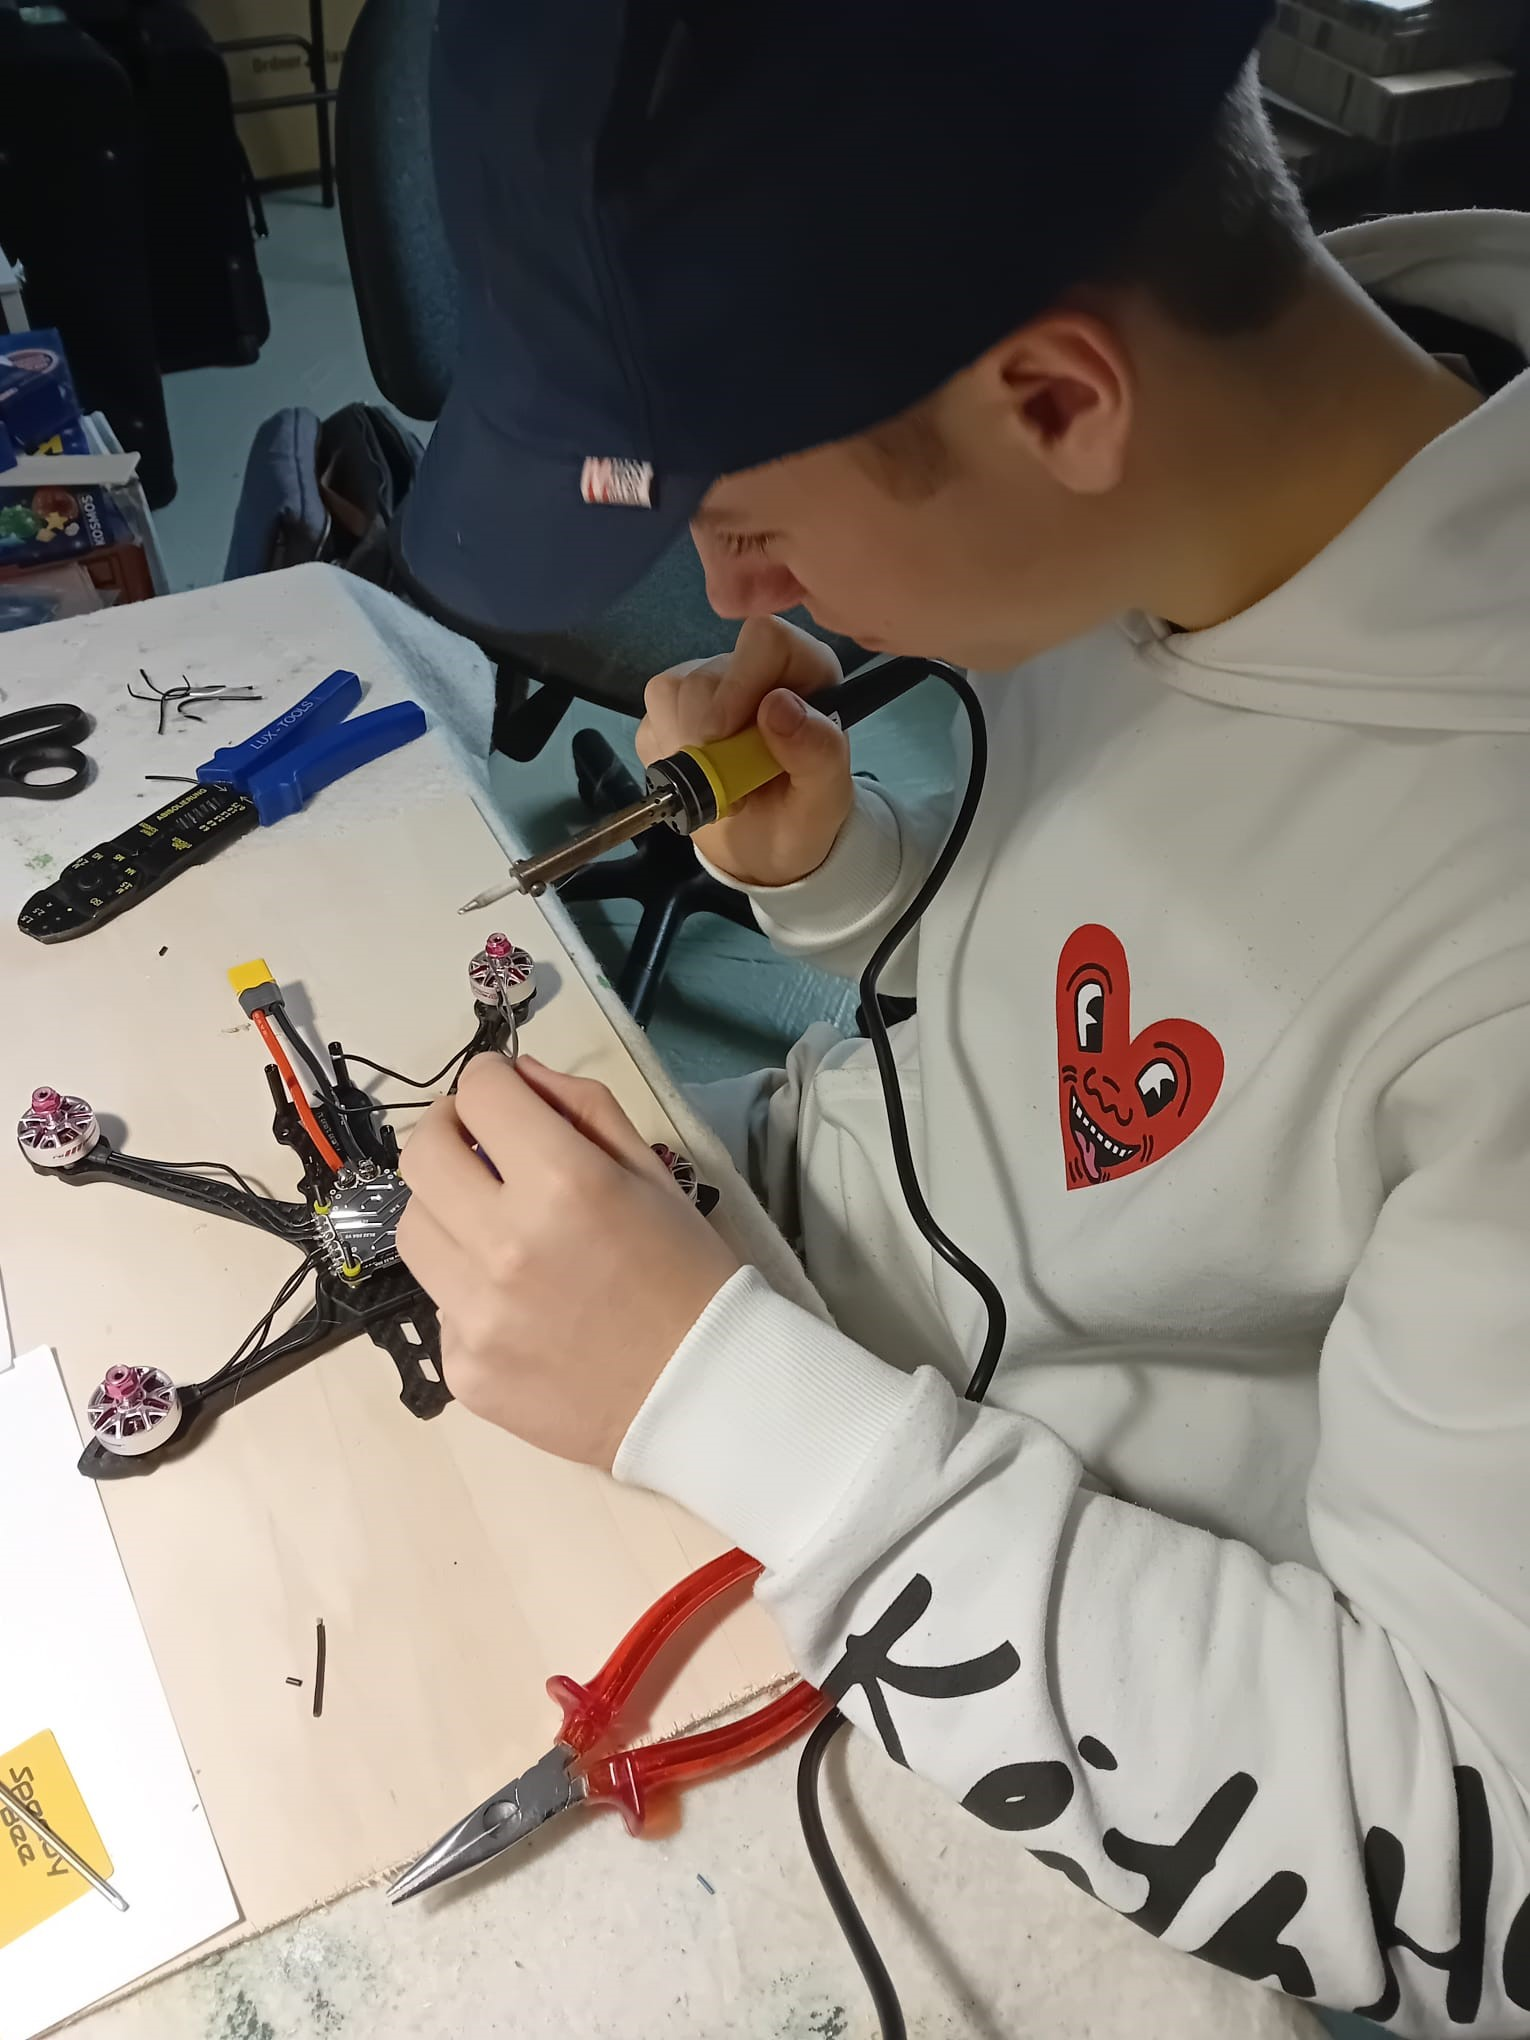
\includegraphics[height=0.3\textheight]{Titelbild_Test.jpg} % Scale to 30% of the height of the text
  \vfill
  Vorgelegt bei:\par
  {\sc\papersupervisor\par}
  \vspace{1cm}
  {\large\paperdate\par}
\end{titlepage}
 %     \
% ------------------

% === INHALTSVERZEICHNIS ===
\tableofcontents %          \
\newpage %                  \
% --------------------------



% =========== START VON STYLING ===========
\onehalfspacing % Zeilenabstand 1.5
\renewcommand{\chaptermark}[1]{\markboth{\MakeUppercase{\thechapter.\ #1}}{}} % Kapitel
\renewcommand{\sectionmark}[1]{\markright{\thesection.\ #1}{}} % Abschnitt
\fancyhead[R]{\rightmark}
\fancyhead[L]{\leftmark}
%\fancyhead[C]{\thepage{}} % Seitennummer
\fancyfoot{}
\fancyfoot[C]{\thepage} % Seitenzahl unten in der Mitte
\fancyhead[L]{\leftmark}
\fancyhead[R]{\rightmark}

\pagestyle{fancy}
% =========== ENDE VON STYLING ============

% === KAPITEL DER ARBEIT ===
\chapter*{Vorwort}

Da wir beide in unserer Freizeit viel mit Drohnen gespielt und uns intensiv mit ihnen befasst haben, stellte sich irgendwann die unabdingbare Frage: \textit{Wie funktionieren Drohnen eigentlich, und wie sind sie aufgebaut?} Um diese Frage zu klären, haben wir uns entschieden, unsere Maturaarbeit diesem faszinierenden Thema zu widmen. Drohnen vereinen zahlreiche Technologien, von moderner Mechanik über ausgeklügelte Elektronik bis hin zu hochentwickelter Software, was sie zu einem spannenden Forschungsfeld macht. Wir möchten sowohl die Hardware als auch die Software einer Drohne genauer untersuchen, um ein tieferes Verständnis für die Funktionsweise dieser Geräte zu entwickeln.

Anfangs hatten wir geplant, das Steuerungsprogramm der Drohne komplett selbst zu schreiben. Doch im Laufe unserer Recherchen haben wir schnell erkannt, dass dies den Rahmen einer Maturaarbeit sprengen würde. Zudem haben wir erkannt, dass dieses Thema von beinahe allen Personen unterschätzt wird und die Entwicklung einer solchen Software ist ein komplexes Unterfangen, das weitreichende Kenntnisse in Programmierung, Steuerungstechnik und Signalverarbeitung erfordert. Stattdessen entschieden wir uns, uns auf den Aufbau der Drohne und die Analyse bestehender Software zu konzentrieren. Wir wollten durch die Untersuchung spezifischer Funktionen und durch gezielte Anpassungen des Drohnencodes die Funktionsweise besser nachvollziehen und gleichzeitig praxisnahe Erfahrungen sammeln.

Unser Ziel ist es, die Technologie einer Drohne umfassend zu analysieren – von der Hardware, die für ihre Bewegungen verantwortlich ist, bis hin zum Code, der für die präzise Steuerung und autonome Funktionalität sorgt. So hoffen wir, ein tieferes Verständnis in diese faszinierende Technologie zu gewinnen.

Abschliessend möchten wir anmerken, dass diese Arbeit auch ein Stück Leidenschaft widerspiegelt. Die Begeisterung, die wir bei der Auseinandersetzung mit Drohnen erleben durften, hat uns durch die anspruchsvollen Phasen des Projekts getragen. Wir sind gespannt, welche Erkenntnisse wir auf unserem Weg, den wir dank unseres Sponsors, dem Altersheim Abendruh \cite{Altersheim}, gehen können, noch gewinnen werden.
\chapter{Einleitung}
\section{Themenvorstellung}
Drohnen haben in den letzten Jahren grosse Fortschritte gemacht und finden Anwendung in unterschiedlichsten Bereichen wie Logistik, Vermessung und Unterhaltung. Für die vielfältigen Einsatzmöglichkeiten ist das Verständnis der Funktionsweise und des Aufbaus einer Drohne von zentraler Bedeutung, nicht zuletzt für die Weiterentwicklung der Technologie. Insbesondere die Entwicklung von Steuermechanismen, wie zum Beispiel eines präzisen Landeschalters, stellt eine grundlegende Herausforderung dar, die praktische und technische Kompetenzen erfordert.
	
\section{Forschungsstand und Problemstellung}
Die Grundlagen der Drohnentechnologie – darunter Aerodynamik, Steuerung und Energiemanagement – sind in gut dokumentiert. Ebenso gibt es zahlreiche technische Ansätze zur Automatisierung einzelner Funktionen wie Start und Navigation. Doch die Frage, wie komplex diese Technologie wirklich ist und wie ein Schalter zur automatisierten Landung programmiert sowie in die bestehende Steuerung integriert werden kann, bildet den Schwerpunkt dieser Arbeit.
	
\section{Ziele der Arbeit}
Das Ziel dieser Arbeit ist es, die Funktionsweise und den Aufbau einer Drohne zu analysieren und einen funktionalen Landeschalter zu entwickeln. Dies umfasst die theoretische Untersuchung der technischen Grundlagen sowie die praktische Umsetzung und Programmierung des Schalters. Durch die Kombination von Theorie und Praxis soll ein besseres Verständnis für die zentralen Komponenten und Steuermechanismen einer Drohne vermittelt werden.

\chapter{Zielsetzung}

Das übergeordnete Ziel dieser Arbeit besteht darin, einen Schalter zu implementieren, der es der Drohne ermöglicht, aus einer beliebigen Höhe automatisch zu landen. Um dieses Ziel zu erreichen, müssen verschiedene Teilziele bearbeitet werden. Diese umfassen das Verständnis des zugrunde liegenden Codes sowie die Implementierung und Optimierung der Fluglogik und des Failsafe-Modus.

\section{Hardware}

Die vorliegende Arbeit zielt darauf ab, die für den Flug essenziellen Hardwarekomponenten zu selektieren und zu montieren, sodass die Drohne danach einwandfrei fliegt. Die Auswahl der Komponenten, zu denen Flugcontroller, Motoren, Sensoren und Akkus zählen, erfolgt mit Bedacht, um eine optimale Leistung und Stabilität der Drohne zu gewährleisten. Die Auswahl der Komponenten ist in der Arbeit unter \autoref{sec:Teile} zu finden. Die Installation der Motoren, Propeller und Sensoren sowie die Verkabelung aller elektrischen Komponenten (siehe hierzu auch: \autoref{ch:ZusammenbauDrohne}) wurde selbstständig geplant und durchgeführt. Im Anschluss an den Zusammenbau erfolgen Versuche, um die korrekte Funktion aller Systeme sicherzustellen und die Implementierung des Schalters zur Landung in der Software zu ermöglichen (siehe hierzu auch: \autoref{sec:tests}).


\begin{comment}

\section{Analyse und Verständnis der Sensordaten}

Danach kommt die Analyse und das Verständnis der Sensordaten, die von der Drohne geliefert werden. Diese Sensordaten stammen aus verschiedenen Sensoren wie Gyroskopen und Beschleunigungsmessern die wichtige Informationen zur Flugstabilität liefern. Für diese Analyse wird die Betaflight-Applikation verwendet, die die Sensordaten in Echtzeit erfasst. \par
Die Sensordaten werden mit der Betaflight-Software erfasst, die speziell für die Konfiguration und Überwachung von Flugcontrollern in Drohnen entwickelt wurde.

Nach der Datenerfassung werden die Sensordaten in Excel (\autoref{sec:tests}) eingetragen, um die Datenverarbeitung und visuelle Analyse zu erleichtern.

Die aufbereiteten Daten werden analysiert, um Muster, Abweichungen und mögliche Instabilitäten im Flugverhalten der Drohne zu identifizieren. Dabei werden insbesondere die Schwankungen in den gemessenen Beschleunigungen und Drehgeschwindigkeiten untersucht.
Ziel ist es, ein fundiertes Verständnis der Sensordaten zu erlangen, um eine Grundlage für die Programmierung der Stabilisationsfunktion zu schaffen. Dies könnte auch die Ermittlung von Schwellenwerten oder die Identifizierung kritischer Flugzustände umfassen.
\end{comment}

\section{Programmierung des Landeschalters für die Drohne}

Das zweite Ziel dieser Arbeit besteht in der Programmierung der Landeschalter-Funktion für die Drohne, deren Zweck darin besteht, beim Umlegen des Landeschalters eine automatische Rückkehr der Drohne auf den Boden und eine sichere Landung zu gewährleisten. Der Prozess der Programmierung gliedert sich in die folgenden Schritte: 

Zunächst wird der bestehende Sourcecode von Betaflight analysiert. Ziel ist die Identifizierung des Teils des Codes, der für die Steuerung der Drohne zuständig ist. Dazu zählen auch die Untersuchung bestehender Algorithmen und Funktionen, die für die Landung genutzt werden könnten, wie etwa die aktuellen Steuerungslogiken, die PID-Regler und der Grundaufbau des Codes, die beim Greifen des Landeschalters nützlich sein könnten.

Nach der Analyse des Sourcecodes wird die Landeschalter-Funktion implementiert. Hierzu werden geeignete Algorithmen entwickelt, die die Drohne beim Umlegen des Landeschalters automatisch in einen sicheren Landeprozess versetzen. Die Algorithmen könnten auf bestehenden Algorithmen basieren, die die Position und den Zustand der Drohne überwachen, um eine sanfte und konstante Landung zu gewährleisten. Diese konstante Landung könnte mit der Abhängigkeit des Barometer kontrollieren und angepasst werden.

Die Funktionalität wird in verschiedenen Testszenarien überprüft, um die Zuverlässigkeit der Drohne in unterschiedlichen Bedingungen sicherzustellen. Die Tests dienen dazu, die korrekte Reaktion der Drohne auf Steuerbefehle und die Sicherheit des Landeprozesses zu gewährleisten, wenn der Landeschalter aktiviert wird. Basierend auf den Ergebnissen der Testszenarien erfolgt eine  Optimierung der Landeschalter-Funktion.


\section{Zusammenfassung der Ziele}

Insgesamt wird sich die Arbeit auf den Zusammenbau und den Landeschalter der Drohne fokusieren, der auf einer fundierten Analyse des Sourcecodes basiert. Durch die Implementierung und Optimierung der Funktion sowie durch Tests wird sichergestellt, dass die Drohne stabil und zuverlässig landet.

\chapter{Technische Einzelheiten der Drohne} 
\section{Die Teile}\label{sec:Teile}

Um die für die Drohnenkonstruktion erforderlichen Komponenten zu bestimmen, wurden umfassende Recherchen durchgeführt, mit dem Ziel, geeignete Drohnenteile zu identifizieren und zu beschaffen. Die in der Arbeit verwendete Drohen ist eine FVP-Racing-Drohen\cite{FPV} im Quadkopter\cite{Quadkopter} Art, jedoch ohne Videobrille und Kamera. 

Im Rahmen dieser Untersuchung wurden die folgenden Teile als relevant eingestuft und anschliessend beschafft. Im Anhang ist eine \hyperref[ch:infoteile]{Tabelle} der Teile mit den wichtigsten Funktion und Eigenschaft zu finden.

\subsection{Akkumulator} \label{sec:Akku} 
Für den Quadkopter wurde eine Batterie des Herstellers OVONIC verwendet. Die Batterie weist eine Spannung von 22,2 Volt auf und ein Gewicht von 222 Gramm. Ihre Funktion besteht in der kontinuierlichen und stabilen Spannungsversorgung sämtlicher elektronischer Komponenten der Drohne. Sie ist für Racing-Drohnen optimiert und gewährleistet so eine besondere Leistungsfähigkeit. Die verwendete Lithium-Polymer (LiPo)-Technologie ist aufgrund ihres vorteilhaften Energie-zu-Gewicht-Verhältnisses für den Einsatz in Drohnen prädestiniert.\cite{Akku} Der Akkumulator besteht aus sechs identischen Zellen. Es gäbe auch kleinere Akkumulatoren, die aus vier Zellen bestehen. Aufgrund der leistungsstarken Motoren, die verbaut wurden, fiel die Entscheidung zugunsten des Systems, das mit sechs Zellen betrieben wird.

\subsection{Motoren}\label{sec:Motoren}

Die Motoren einer Drohne sind von essenzieller Bedeutung für das Abheben und die Steuerung. Mittels einer variierenden Drehrichtung, die sich in ihrer Drehzahl unterscheiden kann, ist eine Bewegung der Drohne in alle Richtungen sowie eine Rotation um die eigene Achse möglich. Für die Konstruktion wurden vier bürstenlose Motoren ausgewählt, die mit 5-Zoll-Propellern kompatibel sind. Diese Motoren sind ebenfalls für Racing-Drohnen geeignet und weisen ein Gewicht von jeweils 30 Gramm auf. \cite{Motorenkauf} Die bürstenlose Bauweise erhöht die Effizienz und Lebensdauer der Motoren. Die Kommutierung erfolgt elektronisch durch einen Controller, der die Phasen der Statorwicklungen zur optimalen Zeit schaltet, um ein kontinuierliches Drehmoment zu erzeugen. \cite{Motorenstudy} Diese präzise Steuerung ermöglicht eine gleichmässige Rotation des Motors sowie eine exakte Leistungsabgabe. Bürstenlose Motoren zeichnen sich durch ein optimales Leistungs-Gewicht-Verhältnis aus, was sie insbesondere für den Einsatz in Racing-Drohnen prädestiniert.


\subsection{Propeller}\label{sec:Propeller} 
\begin{wrapfigure}{r}{0.3\textwidth}  % r für rechts, 0.3\textwidth für Bildbreite
	\centering
	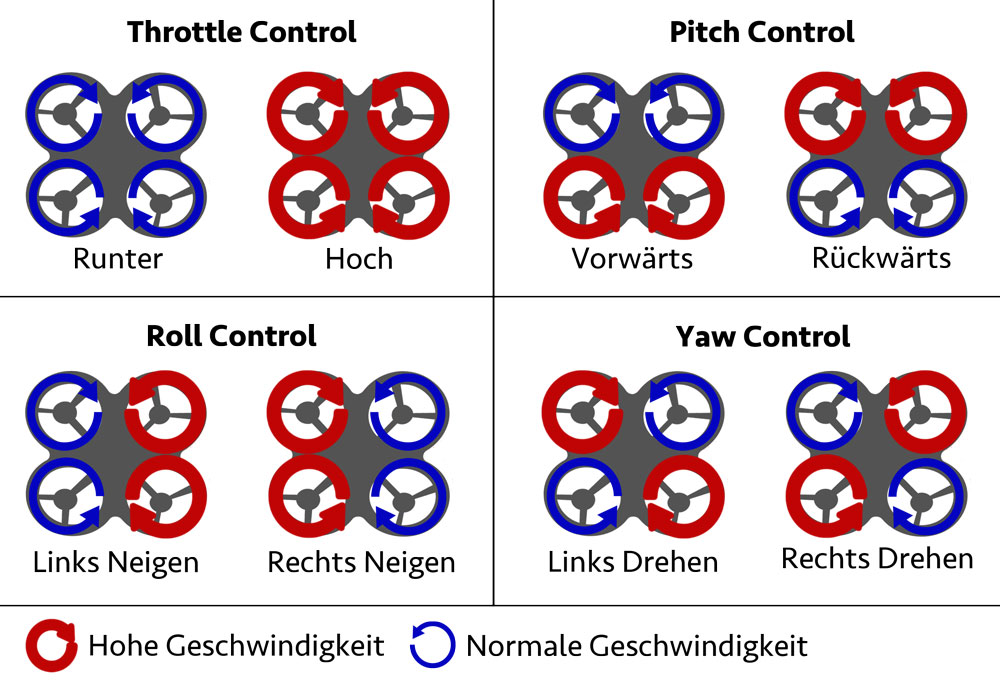
\includegraphics[width=0.28\textwidth]{MotionDE.jpg} % Passt die Bildbreite an
	\caption{Die Grundlagen der Drohnensteuerung}
	\label{fig:motionde}
\end{wrapfigure}
Die für den Flug der Drohne verantwortlichen Propeller erzeugen durch ihre Drehbewegung Schub, der für die Aufrechterhaltung der Flugposition in der Luft erforderlich ist. Die aerodynamische Form der Propellerblätter optimiert die Luftströmung, sodass diese effizient bewegt wird. Bei einem Quadkopter drehen die Propeller über Kreuz jeweils in die gleiche Richtung, was eine unkontrollierte Rotation der Drohne um die Z-Achse verhindert. Dieses Prinzip findet ebenfalls Anwendung bei der gezielten Rotation der Drohne, wie bei \autoref{fig:motionde} gezeigt.

\subsection{Speedy Bee F7 V3 Stack}  \label{sec:F7V3}
Der Flight Controller (FC) stellt das Herzstück der Drohne dar und basiert auf einem leistungsstarken STM32F7-Mikrocontroller. Dieser bietet ausreichend Rechenleistung für die Bewältigung komplexer Steueraufgaben sowie die Verarbeitung von Sensordaten, Steuerbefehlen und Flugalgorithmen. \cite{Stack}

Der Electronic Speed Controller (ESC), der direkt unter dem FC verbaut wurde, regelt die elektrische Leistung von der Batterie zu den Motoren. Die vom FC vorgegeben Motordrehzahl werden durch den ESC praktisch umgesetzt. Der für das Projekt eingebaute Speedy Bee F7 V3 Stack vereint eine Vielzahl von Funktionen in einem Gerät und ist mit einer Vielzahl anderer Komponenten kompatibel. Erwähnenswert sind auch die Sensoren wie die \hyperref[sec:IMU]{IMU} und der \hyperref[sec:Barometer]{Barometer}. Diese befinden sich ebenfalls direkt auf der Platine des Speedy Bee F7 V3 Stacks und werden später noch detaillierter beschrieben.

\subsection{ELRS-Empfänger} \label{sec:ELRS-Empfänger}
Der Express Long Range System (ELRS)-Empfänger \cite{ELRS} fungiert als Antenne der Drohne. Er empfängt Steuerbefehle über eine Frequenz von 2.4 Gigaherz und bietet den Vorteil einer stabilen Verbindung über grössere Entfernungen. Der ELRS-Empfänger wandelt die Radiofrequenzsignale in elektrische Impulse um, die vom FC in Steuerbefehle für den ESC umgesetzt werden. Auf diese Weise wird ein Signal erzeugt, wenn an der Fernbedienung ein Stick bewegt wird.

\subsection{Fernbedienung}  
Die RadioMaster Boxer ist eine vielseitige und moderne Funkfernbedienung, die speziell für den Einsatz mit Drohnen und anderen ferngesteuerten Modellen entwickelt wurde. Mit einem Frequenzbereich von 2,4 Gigaherz ermöglicht sie eine stabile Verbindung zwischen Sender und Empfänger\cite{RadioController}. Sie unterstützt bis zu 16 Kanäle, was eine präzise Steuerung selbst bei komplexen Anforderungen sicherstellt \cite{RadioController}. Ein besonderes Merkmal ist die Auswahl zwischen zwei internen Hochfrequenzmodulen: einem ExpressLRS (ELRS)-Modul\footnote{ExpressLRS (ELRS) ist ein modernes, Open-Source-Funkübertragungssystem, das speziell für ferngesteuerte Modelle wie Drohnen und RC-Fahrzeuge (Remote controlle Fahrzeuge) entwickelt wurde. Es bietet eine extrem geringe Latenz(Verzögerung) von nur 4–8 ms, eine hohe Reichweite von mehreren Kilometern und eine robuste Signalübertragung dank der LoRa-Modulationstechnologie (LoRa = Long Range). ExpressLRS unterstützt Frequenzbänder wie 2,4 Gigaherz für schnelle Reaktionen und 900 MHz für maximale Reichweite. Durch seine Flexibilität, Anpassungsfähigkeit und Kompatibilität mit verschiedenen Geräten ist ELRS ideal für FPV-Racing, Long-Range-Flüge sowie industrielle Anwendungen. Zudem zeichnet es sich durch geringen Stromverbrauch und eine aktive Entwickler-Community aus.} und einem 4-in-1/CC2500 Multi-Protokoll-Modul, wodurch eine breite Kompatibilität mit verschiedenen Empfängern gewährleistet wird \cite{ATOMRC}.

Die technische Ausstattung der RadioMaster Boxer umfasst einen leistungsstarken STM32\-F407VGT6-Prozessor mit 1 MB Flash-Speicher und 192 KB RAM, der eine schnelle und zuverlässige Signalverarbeitung ermöglicht. Vorinstalliert ist die Open-Source-Firmware EdgeTX, die durch ihre Flexibilität und Anpassbarkeit überzeugt. %Zusätzlich ist die Fernbedienung ergonomisch gestaltet und mit hochwertigen Hall-Gimbals \footnote{Hall-Gimbals sind Steuerknüppel, die mit Hall-Sensoren arbeiten, um Bewegungen präzise und berührungslos zu messen. Die Position des Hebels wird dabei durch Veränderungen im Magnetfeld erfasst, ohne dass es zu mechanischem Verschleiss kommt, wie er bei herkömmlichen Potentiometern zu beobachten ist. Ihre Langlebigkeit, das sanfte Steuergefühl und die Möglichkeit der individuellen Anpassung von Härte und Selbstzentrierung sind signifikante Vorteile. Hall-Gimbals finden vor allem in Fernbedienung für Drohnen oder RC-Geräte Anwendung, wo Präzision und Zuverlässigkeit von entscheidender Bedeutung sind.} ausgestattet, die eine präzise Steuerung und ein komfortables Benutzererlebnis bieten. 
Die Energieversorgung kann wahlweise über eine 7,4V 2-Zellen Lithium-Polymer-Batterie oder zwei 3,7V 18650 Lithium-Ionen-Zellen erfolgen, wodurch eine flexible und zuverlässige Nutzung sichergestellt wird.\cite{RadioController}\cite{ATOMRC}

Im Kontext der Drohnennsteuerung nimmt die Wahl der Fernbedienung eine entscheidende Rolle ein. Funkfernbedienung, wie die RadioMaster Boxer, senden Signale an die Drohne, um diese in Bezug auf Richtung, Höhe und Geschwindigkeit zu steuern. Die Drohne empfängt diese Signale und setzt sie um, indem sie die Motoren entsprechend ansteuert \cite{Steuerung}. Dafür ist es essenziell, dass sowohl die Fernbedienung als auch der Empfänger dieselbe Sprache sprechen, also dass sie das gleiche Kommunikationsprotokoll verwenden – in diesem Fall ExpressLRS. % Die Steuerung wird durch Gyroskope und Flugsteuerungssysteme ergänzt, die Daten von Sensoren verarbeiten und die Stabilität der Drohne in der Luft gewährleisten. Diese Systeme sind von entscheidender Bedeutung, um automatisierte Bewegungen, präzise Manöver und Stabilisierung auch bei Störungen wie Wind oder Turbulenzen sicherzustellen \cite{Steuerung}.

Die Zuverlässigkeit und Präzision der Funkverbindung sind dabei von entscheidender Bedeutung, da Störungen in der Funkverbindung potenziell gefährliche Situationen verursachen könnten. Hochwertige Fernbedienungen wie die RadioMaster Boxer sind daher sehr wichtig\cite{Steuerung}. Ihre Vielseitigkeit und Leistungsfähigkeit machen sie zu einer idealen Wahl für die anspruchsvolle Steuerung von Drohnen in wissenschaftlichen und technischen Projekten.


\subsection{Smoke Stopper} \label{sec:Smoke Stopper}
Der Smoke Stopper\cite{SmokeStopper} ist ein Kurzschlussschutz, der bei einem Kurzschluss, also dem ungewollten Kontakt zweier nicht verbundener Leitungen (0 Ohm), eingreift und den Stromkreis unterbricht. Der Smoke Stopper wurde in diesem Fall zur Absicherung der Drohne im Falle einer fehlerhaften Lötstelle eingesetzt.\footnote{Das Projekt verlief planmässig, sodass der Smoke Stopper nicht aktiv wurde.}

\subsection{Kondensator} \label{sec:Kondensator}
Ein Kondensator ist ein elektronisches Bauteil, das in zahlreichen Geräten Anwendung findet. Er speichert elektrische Energie kurzzeitig und gleicht dadurch Schwankungen im Stromfluss aus. Dies schützt die Bauteile im Stromkreis vor Spannungsspitzen und sorgt gleichzeitig für einen gleichmässigeren Stromfluss, was zu einer stabileren und zuverlässigeren Leistung führt. Ein passender Kondensator war dem Flight Controller bereits beigelegt und in diesem Projekt verwendet. 

\subsection{Frame}   \label{sec:Frame}
Der Frame \cite{Frame} stellt die Struktur, das Gestell der Drohne dar, an dem alle Komponenten befestigt werden. Der Rahmen besteht aus Kohlefaser, einem leichten, aber robusten Material. Der Rahmen ist im Deadcat-Design\cite{fpv24deadcatframes} konzipiert, was bedeutet, dass die Motoren in einem diagonalen Layout angeordnet sind, wobei die vorderen und hinteren Arme weiter voneinander entfernt sind als die seitlichen Arme. Dieses Design verbessert das Sichtfeld der FPV-Kamera und reduziert die Störung durch Propeller im Kamerabild. Wichtig war, dass der Frame sowohl leicht als auch robust war, was er eindeutig erfüllt.

\section{Die Sensoren}\label{sec:Sensoren}

Die Integration von Sensoren in die Konstruktion einer Drohne ermöglicht die Schaffung eines komplexen Systemes, das als "Gehirn" der Drohne bezeichnet werden kann. 
Die Funktionalität ermöglicht präzises Fliegen, automatische Funktionen und verbessert die Steuerung sowie die intelligenten Fähigkeiten der Drohne, sich selbst zu regulieren und steuern. 

\subsection{IMU}  \label{sec:IMU}
Die Interial Measurement Unit (IMU) fungiert als Beschleunigungsmesser im Flugcontroller. Sie misst, wie schnell und in welche Richtung sich die Drohne dreht. Dank der IMU ist die Drohne stets in der Lage, ihre Ausrichtung während des Flugs präzise zu bestimmen und entsprechend zu korrigieren, um stabil zu fliegen. Die IMU kann als das innere Gleichgewichtsorgan betrachtet werden, das die Drohne auf Kurs hält, vergleichbar mit dem Innenohr des Menschen. Es besteht aus einem Beschleunigungssensor und einem Gyroskop, das die lineare Beschleunigung sowie die Winkelgeschwindigkeit der Drohne in drei Raumrichtungen (x, y, z) misst. Der Beschleunigungssensor misst die lineare Beschleunigung und der durch die Gravitation verursachten Beschleunigung. Er erfasst Änderungen in der Geschwindigkeit (also Beschleunigungen) und kann durch Integration dieser Messwerte die Geschwindigkeit berechnen. Meistens wird ein kapazitiver\footnote{Ein kapazitiver Drucksensor verwendet zwei parallel angeordnete Platten, von denen eine fest und die andere druckempfindlich ist. Wenn Druck auf die bewegliche Platte ausgeübt wird, verändert sich der Abstand zwischen den Platten und damit die Kapazität des Systems. Diese Kapazitätsänderung wird in ein elektrisches Signal umgewandelt. Kapazitive Drucksensoren zeichnen sich durch hohe Genauigkeit und Langzeitstabilität aus und werden daher in medizinischen und sicherheitskritischen Anwendungen bevorzugt eingesetzt.\cite{Capacitive_vs_Piezoresistive}} oder piezoresistiver\footnote{Ein piezoresistiver Drucksensor arbeitet, indem er die Widerstandsänderung eines Materials misst, wenn Druck auf eine Siliziummembran ausgeübt wird. Auf dieser Membran befinden sich vier Widerstände, die sich verformen, sobald Druck ausgeübt wird, was zu einer Änderung des elektrischen Widerstands führt. Diese Veränderung wird durch eine Wheatstone-Brücke in ein elektrisches Signal umgewandelt.\cite{Capacitive_vs_Piezoresistive} Piezoresistive Drucksensoren sind aufgrund ihrer geringen Produktionskosten weit verbreitet und finden Anwendung in der Automobilindustrie, in Haushaltsgeräten und in Konsumgütern.} Beschleunigungssensor eingesetzt. Das Gyroskop hingegen misst die Winkelgeschwindigkeit um die drei Achsen. Häufig kommt ein MEMS-Gyroskop (Micro-Electro-Mechanical-Systems) zum Einsatz, das auf dem Coriolis-Effekt basiert. 	Dabei detektiert das Gyroskop Rotationsbewegungen, indem es die durch die Rotation erzeugten Corioliskräfte auf winzige, bewegliche Strukturen innerhalb des Sensors misst. Diese Kräfte werden in elektrische Signale umgewandelt, die die Winkelgeschwindigkeit in den drei Raumrichtungen präzise erfassen."\footnote{Die Corioliskraft ist die Kraft, die durch die Rotation der Erde um ihre eigene Achse erzeugt wird. Auf der Nordhalbkugel werden die Teilchen nach rechts und auf der Südhalbkugel nach links abgelenkt. Hurrikane oder der Wasserabfluss drehen auf der Nordhälfte der Erde andersherum als auf der Südhälfte. \cite{Coriolis}} Durch die Kombination der Daten von Beschleunigungssensor und Gyroskop kann die exakte Orientierung der Drohne im Raum ermittelt werden. Dies geschieht, indem die Daten durch ein Kalman-Filter\footnote{Der Kalman-Filter ist ein mathematisches Verfahren zur Schätzung von Systemzuständen, die nicht direkt messbar sind, auf der Grundlage fehlerhafter Beobachtungen. Er kombiniert in jedem Schritt neue Messungen mit bisherigen Schätzungen, um den Fehler zu minimieren. Besonders ist, dass der Filter neben den Schätzwerten auch die Unsicherheiten und Korrelationen zwischen den Schätzfehlern berücksichtigt. Dadurch kann er dynamische Grössen wie Position und Geschwindigkeit präzise schätzen. Der Kalman-Filter wird in vielen technischen Bereichen eingesetzt, etwa zur Positionsbestimmung oder in elektronischen Steuerungssystemen. \cite{Kalman}} verarbeitet werden, um eine optimale Schätzung des Zustands der Drohne zu erhalten. Diese IMU-Daten bilden die Grundlage für die Regelung der Fluglage und zur Stabilisierung der Drohne.

\subsection{Barometer}  \label{sec:Barometer}
Das Barometer misst den Luftdruck, was für eine Drohne in bestimmten Gebieten von enormer Relevanz sein kann, da die Höhe über dem Boden möglichst genau ermittelt werden muss. Dies ist beispielsweise im „Altitude-Hold“-Modus wichtig, bei dem die Drohne automatisch ihre Höhe beibehält. In dieser Maturaarbeit spielt das Barometer ebenfalls eine zentrale Rolle, da es die Berechnung der Sinkgeschwindigkeit im Falle eines Fail-Safes ermöglicht. Diese Anpassung des Fail-Safe-Modus ist ein wesentlicher Bestandteil der vorliegenden Arbeit. Meist wird das Barometer zusätzlich durch ein GPS ergänzt, das ebenfalls die Höhe über dem Meeresspiegel misst. Diese Kombination ermöglicht eine deutlich höhere Genauigkeit. In diesem Fall muss jedoch auf ein GPS verzichtet werden, da der Flight Controller (FC) kein integriertes GPS besitzt und aus Komplexitätsgründen bewusst auf ein externes GPS verzichtet wurde.
% \chapter{Gitcode Anleitung}\label{sec:gitcode}
\section{Jamilszeug}
\lstinputlisting[
label=lst:gitcomposory,
caption={[gitcomposory]Eine Anleitung git zu gebruachen},
% linerange={88-93},firstnumber=88
]{code/git.sh}%brüche mer nid
\chapter{Zusammenbau der Hardware} \label{ch:ZusammenbauDrohne}
Der Zusammenbau einer Drohne erfordert Verständnis der einzelnen Komponenten und deren Integration zu einem funktionsfähigen System. Im Folgenden wird der Prozess des Zusammenbaus der Drohne in seinen wesentlichen Schritten beschrieben.

\section{Auswahl und Bestellen der Teile}
Die sorgfältige Selektion der Komponenten stellt einen wichitgen Schritt im Konstruktionsprozess der Drohne dar. Die Auswahl der Komponenten, wie beispielsweise Akkumulator, Motoren, Propeller, Flight Controller, Frame und Zubehör, erfolgt unter Berücksichtigung der spezifischen Anforderungen an die Drohne sowie ihrer geplanten Einsatzgebiete. Der Grund, weshalb hier eine klassische RC-Drohne zusammengebaut wurde, liegt in ihrer weiten Verbreitung. Dadurch steht eine breite Auswahl an Komponenten sowie detaillierte Beschreibungen und Dokumentationen zur Verfügung.

Der Selektionsprozess wurde in mehreren aufeinander aufbauenden Schritten durchgeführt. Zunächst wurden die Anforderungen an die Drohne definiert. Diese Anforderungen determinierten die notwendigen Merkmale der einzelnen Komponenten. In dieser Arbeit waren etwa eine hohe Leistungsfähigkeit der Motoren, ein leichtgewichtiger Frame sowie präzise Manöver von Bedeutung.
  
Die darauf folgende Recherche nach geeigneten Komponenten umfasste eine ausführliche Analyse von Bewertungen, Spezifikationen und Erfahrungsberichten aus Foren, Fachartikeln und YouTube-Videos, um die optimale Auswahl zu treffen. Im Anschluss wurden mehrere Optionen für jedes Bauteil hinsichtlich Preis, Leistung, Kompatibilität und Verfügbarkeit verglichen. Die finale Auswahl erfolgte unter Berücksichtigung des Projektbudgets, um die Balance zwischen Qualität und Kosten zu wahren. Nach erfolgter Entscheidung wurden die benötigten Teile (\autoref{sec:Teile}) bei den Händlern bestellt. Hier wurde vor allem AliExpress genutzt, da die Plattform eine grosse Auswahl an technischen Bauteilen bietet und in diesem Fachgebiet besonders günstige Preise hat

Im Rahmen des Selektionsprozesses zeigen sich jedoch auch diverse Herausforderungen. Zu den am häufigsten auftretenden Problemen zählten Fragen der Kompatibilität, da eine reibungslose Interaktion zwischen den Komponenten nicht gewährleistet werden konnte. So musste beispielsweise die Spannung des Akkumulators mit den Anforderungen des Flight Controllers und der Motoren übereinstimmen. Darüber hinaus stellte das vorgegebene Gewicht der Drohne eine Herausforderung dar, da diese einerseits leicht genug sein sollte, um eine hohe Agilität zu gewährleisten, andererseits aber auch stabil und leistungsfähig bleiben musste. Zudem muss man bei Drohnen eine Prüfung absolvieren, wenn diese ein bestimmtes Gewicht überschreitet \cite{Prüfung}. Die zusammengebaute Drohne fällt hierbei in die Drohnenklasse C4, weshalb bestimmte Sicherheitsmassnahmen beim Flug eingehalten werden müssen und der Kompetenznachweis A3 erbracht werden muss, der um diese Arbeit durchzuführen von Jamil Sostizzo erlangt wurde.
 
Die sorgfältige Planung und Recherche in dieser Phase waren entscheidend, um hochwertige und kompatible Bauteile auszuwählen. Der Grundstein für eine funktionsfähige und leistungsstarke Drohne, die den Anforderungen des Projekts gerecht wird, konnte hiermit gelegt werden.\hyperref[infoteile]{ Im Anhang sind die Verschiedenen Komponenten erneut in Listenform zu finden}

\section{Vorgehen}

 Zu Beginn ist die Montage des \hyperref[sec:Frame]{Rahmens} (Frame), der als Trägerstruktur dient wichtig. Der Rahmen, der aus leichtem und widerstandsfähigem Kohlefaser-Material besteht, wird zunächst verschraubt. Der Rahmen ist die Basis für die Installation der anderen Komponenten.

Im nächsten Schritt wurden die \hyperref[sec:Motoren]{Motoren} an den vorgesehenen Stellen am Rahmen befestigt. Die bürstenlosen Motoren müssen fest und vibrationsfrei montiert werden, um eine präzise Steuerung zu ermöglichen. 
Der \hyperref[sec:F7V3]{Flight Controller (FC)}, das zentrale Steuerungselement der Drohne, wird danach sicher in der Mitte des Rahmens positioniert. Dieser Controller verbindet die verschiedenen Sensoren und elektronischen Komponenten und sorgt für die Echtzeitverarbeitung der Flugsteuerung. Gleichzeitig wird der \hyperref[sec:F7V3]{Electronic Speed Controller (ESC)} installiert, der die Leistung der Motoren steuert. Der ESC ist über Kabelverbindungen sowohl mit den Motoren als auch mit dem Akkumulator und dem Flight Controller verbunden. Bei der Verkabelung muss darauf geachtet werden, dass die Verbindungen sauber und korrekt verlötet werden, um Kurzschlüsse zu vermeiden. 
Sobald die Hauptsteuerungseinheit vollständig gelötet wurden, erfolgt die Verlötung mit dem \hyperref[sec:ELRS-Empfänger]{Express Long Range System (ELRS)-Empfänger}, dem Stromkabel und dem Kondensator.
Anschliessend wird der \hyperref[sec:Akku]{Akkumulator} über den \hyperref[sec:Smoke Stopper]{ Smoke Stopper} an die Drohne angeschlossen. 
Bei dieser Arbeit waren alle Lötstellen sauber und der Smoke Stopper kam nicht zum Einsatz. Das Bedeutet, die Motoren haben gedreht und dadurch Töne entstehen lassen. Dies geschieht immer, wenn die Drohne über den Akkumulator mit Strom versorgt wird.

Zum Schluss wird jeder Motor mit einem \hyperref[sec:Propeller]{Propeller}  versehen. Es ist wichtig, dass die Propeller in der korrekten Drehrichtung montiert werden, um die Stabilität des Fluggeräts zu gewährleisten. Propeller, die in entgegengesetzte Richtungen drehen, verhindern ein ungewolltes Rotieren der Drohne um ihre eigene Achse (\autoref{fig:motionde}).

\section{Probleme}
Zu Beginn war die grösste Hürde herauszufinden welche Komponente über welchen Weg wohin zu löten waren. Danach war das Löten so wie das Zusammenfügen kein Problem mehr. Um dieses Problem zu überwinden erforderte es eine gründliche Untersuchung der Schaltpläne und eine Auseinandersetzung mit den Spezifikationen der Komponenten. Hierbei war das Board Manual\cite{BoardManual} sehr aufschlussreich. Zudem haben wir unsere Recherche gut Dokumentiert

\begin{figure}[h!]
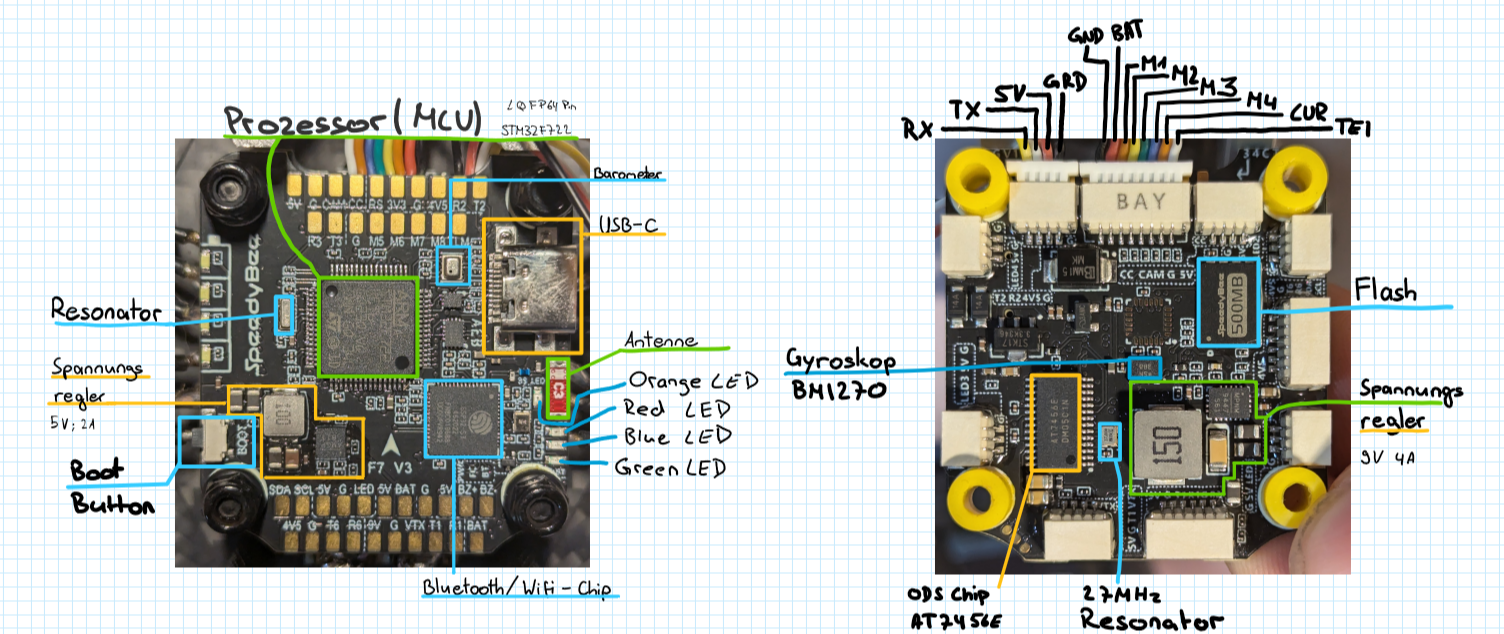
\includegraphics[width=0.635\textheight]{OneNote1&2.png}
\caption{Beschriftung des Prozessors}
\label{fig:OneNote1&2}
\end{figure}
	
Nachdem diese Hürde überwunden war, war der eigentliche Lötprozess und das anschliessende mechanische Zusammenfügen der Bauteile vergleichsweise unkompliziert.

Bei einigen später durchgeführten Tests, stürzte unsere Drohne mehrmals ab und die Propeller brachen. Die Schwierigkeit beim Zusammenbau war sehr unterschiedlich. Am schwierigsten war es, als durch einen Unfall die Verbindung des Motorenkabels, des Stromzufuhrkabels sowie des Kondensators gelöst wurde. Diese Lötstellen mussten zuerst gereinigt und danach neu gelötet werden. Beim Motorenkabel war dies kein Problem. Beim Stromkabel und dem Kondensator hatte man jedoch nur eingeschränkten Zugang, und dazu kam, dass sich die Lötstelle nicht richtig säubern liess. Wir haben versucht sie mit Alkohol zu säubern und abzuschleifen, doch alles vergebens. Die Stromzufuhr und der Kondensator hielten nicht. Nach den Hilfsversuchen von zwei Lehrern sah die Situation immer noch nicht besser aus, weshalb man sich entschloss, professionelle Hilfe in Anspruch zu nehmen. Es wurde Kontakt zum Sponsor der Maturaarbeit, dem Altersheim Abendruh \cite{Altersheim}, aufgenommen, um nach einem Elektriker zu fragen. Dieser reparierte die Drohne im Handumdrehen, und sie funktionierte wieder einwandfrei.

\section{Fazit}

Zusammenfassend lässt sich feststellen, dass der Bau der Drohne ein gewisses Fingerspitzengefühl braucht, ansonsten vergleichsweise leicht durchführbar ist. Trotz anfänglicher Herausforderungen bei der Identifizierung der Teile und korrekten Lötpunkte konnten durch eine sorgfältige Planung alle Probleme gelöst werden.
Die gewählten Bauteile haben sich, wie vorausgesehen, als gut kompatibel erwiesen. Insgesamt erfüllt die Drohne die gestellten Anforderungen und ist bereit für weitere Tests und den praktischen Einsatz.








	
\chapter{Einrichten der Fernbedienung} \label{ch:fernbedieungn}
Der blosse Zusammenbau der Hardware reicht natürlich nicht aus, um eine voll funktionsfähige Drohne zu schaffen. In diesem Fall muss noch die reibungslose Kommunikation zwischen der Fernbedienung und dem Empfänger auf der Drohne gewährleistet werden. Dazu benötigt man eine kompatible Firmware sowohl auf der Fernbedienung als auch auf dem Empfänger.

\section{Die Fernbedienung (Sender)}
Zur korrekten Installation der Firmware, die speziell für die Fernbedienung erforderlich ist, muss zunächst die Firmware in Form einer LUA-Datei erstellt werden. Da in dieser Arbeit das Kommunikationsmodell ExpressLRS verwendet wird, lässt sich mit relativ geringem Aufwand über den ExpressLRS Configurator eine funktionsfähige Firmware erstellen, die speziell für das jeweilige Funkgerät angepasst ist. Um die Firmware nun auf die Fernbedienung zu übertragen, gibt es verschiedene Vorgehensweisen. In diesem Fall wurde über das Einstellungsmenü der Fernbedienung ein WLAN eingerichtet, in das man sich einloggen konnte. Sobald dies geschehen war, öffnete sich eine Webseite, auf der die bereits erstellte Firmware hochgeladen und somit auf die Fernbedienung übertragen werden konnte.

Bei der Ausführung traten grundsätzlich keine grösseren Schwierigkeiten auf, was den Prozess effizient gestaltete und somit wenig Zeit in Anspruch nahm.

\section{Der Empfänger}
Der Empfänger selbst ist ein externes Modul, das an die FC (Flight Controller) angelötet wurde. Im Fall dieser Arbeit wurde der Empfänger an den UART-2 \footnote{UART (Universal Asynchronous Receiver and Transmitter) ist ein Kommunikationsprotokoll, das eine serielle Datenübertragung zwischen zwei Geräten ermöglicht, ohne eine externe Taktung. Es nutzt Start- und Stop-Bits sowie optional ein Parity-Bit zur Fehlererkennung.\cite{UART}} Anschluss angelötet, wie es im Board-Manual\cite{BoardManual} beschrieben ist. Dieser UART wird später noch wichtig werden, da dem FC mitgeteilt werden muss, von welchem Anschluss er das Signal der Fernbedienung empfangen soll. Der eigentliche Vorgang zur Erstellung der Firmware ist im Wesentlichen identisch zum vorherigen Vorgehen. Diesmal muss jedoch über den ExpressLRS Configurator eine BIN-Datei erstellt werden, da auf dem Empfänger ein kleiner Mikroprozessor verbaut ist, der nur Binärdateien lesen kann. Um die erstellte Firmware auf den Empfänger zu laden, muss dieser mit Strom versorgt werden, und man muss eine Minute warten. Nach einer Minute ohne Signal einer Fernbedienung wechselt der Empfänger in einen anderen Modus, in dem er ein eigenes WLAN erstellt. Den Übergang in diesen Modus erkennt man an der schnelleren Blinkfrequenz der LED am Empfänger. Sobald man sich mit dem WLAN verbunden hat, öffnet sich erneut eine Webseite unter der IP-Adresse 10.0.0.1, auf der die zuvor erstellte Firmware hochgeladen werden kann. Dieser Vorgang verlief im Wesentlichen ebenfalls ohne grosse Schwierigkeiten.

\section{Probleme}
Natürlich verlief nicht alles völlig reibungslos. Der Flash-Speicher des Empfängers war zu klein, um die neueste Version der ExpressLRS-Firmware zu installieren. Deswegen läuft auf dem Empfänger die ältere Version 3.3.0, da diese weniger Speicherplatz benötigt. Zu Beginn war noch unklar, dass auch der Sender exakt dieselbe Firmware-Version benötigt, da andernfalls keine Kommunikation zwischen den Geräten möglich ist. Nach dieser Erkenntnis wurde auf der Fernbedienung ebenfalls die Version 3.3.0 installiert, und das Problem war behoben.





\chapter{Programmierung der Firmware} \label{ch:Firmware}

\section{Genutzte Applikationen und Webseiten}

Im Rahmen der Durchführung der Maturaarbeit wurden eine Vielzahl von Applikationen und Webseiten genutzt, die den Arbeitsprozess massgeblich unterstützten und die Umsetzung der verschiedenen Projektteile ermöglichten. %Zu den wichtigsten Tools gehörten sowohl Software-Anwendungen als auch Online-Plattformen, die jeweils eine spezifische Funktionalität erfüllten und zur Effizienzsteigerung beitrugen.

Zunächst wurde GitHub\cite{github} als zentrale Plattform für die Versionskontrolle und Zusammenarbeit verwendet. GitHub ermöglichte das einfache Verwalten von Code-Versionen, das Teilen von Projektdateien mit anderen Mitwirkenden und das Verfolgen von Änderungen im Projektverlauf. Die Integration von GitHub in die Entwicklungsumgebung erleichterte die Zusammenarbeit und die Synchronisation zwischen verschiedenen Geräten. 

Für die Entwicklung und das Testen von Softwareanwendungen so wie das Verwenden von Git wurde das Betriebssystem Ubuntu\cite{ubuntuWSL} eingesetzt. Dieses Betriebssystem wurde vom Betreuer dieser ausdrücklich für die Weiterentwicklung der Firmware und dem Versionsaustausch empfohlen. Die Verwendung von Windows Subsystem for Linux (WSL)\cite{ubuntuWSL} ermöglichte es, eine Linux-Umgebung auf einem Windows-System zu betreiben, wodurch die Nutzung von Linux-Tools und -Befehlen innerhalb von Windows möglich wurde. Dies stellte eine effiziente Lösung für die plattformübergreifende Entwicklung dar.

Für die eigentliche Programmierung und Entwicklung wurde Visual Studio Code (VS Code)\cite{microsoftstore} als Code-Editor eingesetzt. Visual Studio Code bietet durch eine Vielzahl von Erweiterungen (Extensions) eine flexible und leistungsfähige Arbeitsumgebung. Insbesondere die Unterstützung für verschiedene Programmiersprachen, die Möglichkeit zur Code-Vervollständigung, das Debugging und die Integration von Git machten VS Code zu einem unverzichtbaren und starken Werkzeug.

Zur Analyse und Konfiguration von Drohnenflugsteuerungen wurde der Betaflight Configurator\cite{betaflightapp} verwendet. Diese Anwendung ermöglicht die Anpassung zentraler Flight-Controller-Einstellungen sowie das präzise Feintuning von Drohnenparametern, die für eine vollständige Konfiguration und Flugfähigkeit der Drohne unverzichtbar sind. Die App erleichterte das Testen und Optimieren der Drohnensteuerung sowie die Datenanalyse.

Für die allgemeine Recherche und das Sammeln von Informationen spielte die Websuche eine zentrale Rolle. Sie half dabei, schnell auf relevante Artikel, technische Dokumentationen und Lösungen für auftretende Probleme zuzugreifen.

Weiterhin wurden Videos als Lernressourcen genutzt. Viele komplexe technische Aspekte, wie das Einrichten von Entwicklungsumgebungen oder das Verständnis von Programmiersprachen, wurden durch Tutorials und Anleitungen in Videoform vertieft.

Abschliessend wurde TeXstudio\cite{texstudio} als Texteditor für die Erstellung der Maturaarbeit verwendet. TeXstudio ist eine beliebte LaTeX-Umgebung, die eine benutzerfreundliche Oberfläche und zahlreiche Features für die effiziente Arbeit mit LaTeX-Dokumenten bietet. Besonders die umfassende Unterstützung von LaTeX-Befehlen erleichterten das Erstellen und Formatieren des Dokuments.

%Die Kombination dieser Applikationen und Webseiten ermöglichte eine effiziente und gut strukturierte Umsetzung der Maturaarbeit und trug entscheidend zum Erfolg des Projekts bei.


\begin{comment}
\section{Analyse der Daten}\label{sec:Tests}

Ziel der Versuche war es, die Neigungswinkel der Drohne in den Achsen \textit{Pitch} und \textit{Roll} zu messen und die entsprechenden Sensordaten zu analysieren. Für die Untersuchungen wurden systematisch festgelegte Neigungswerte in Grad für die Achsen Pitch und Roll verwendet. Diese Variation diente dazu, die Auswirkungen auf die Flugausrichtung der Drohne zu erfassen. Die gemessenen Sensordaten aus den Achsen \(x\), \(y\) und \(z\) wurden aufgezeichnet, um Rückschlüsse auf die Stabilität und das Verhalten der Drohne in unterschiedlichen Neigungssituationen zu ziehen.

\vfill
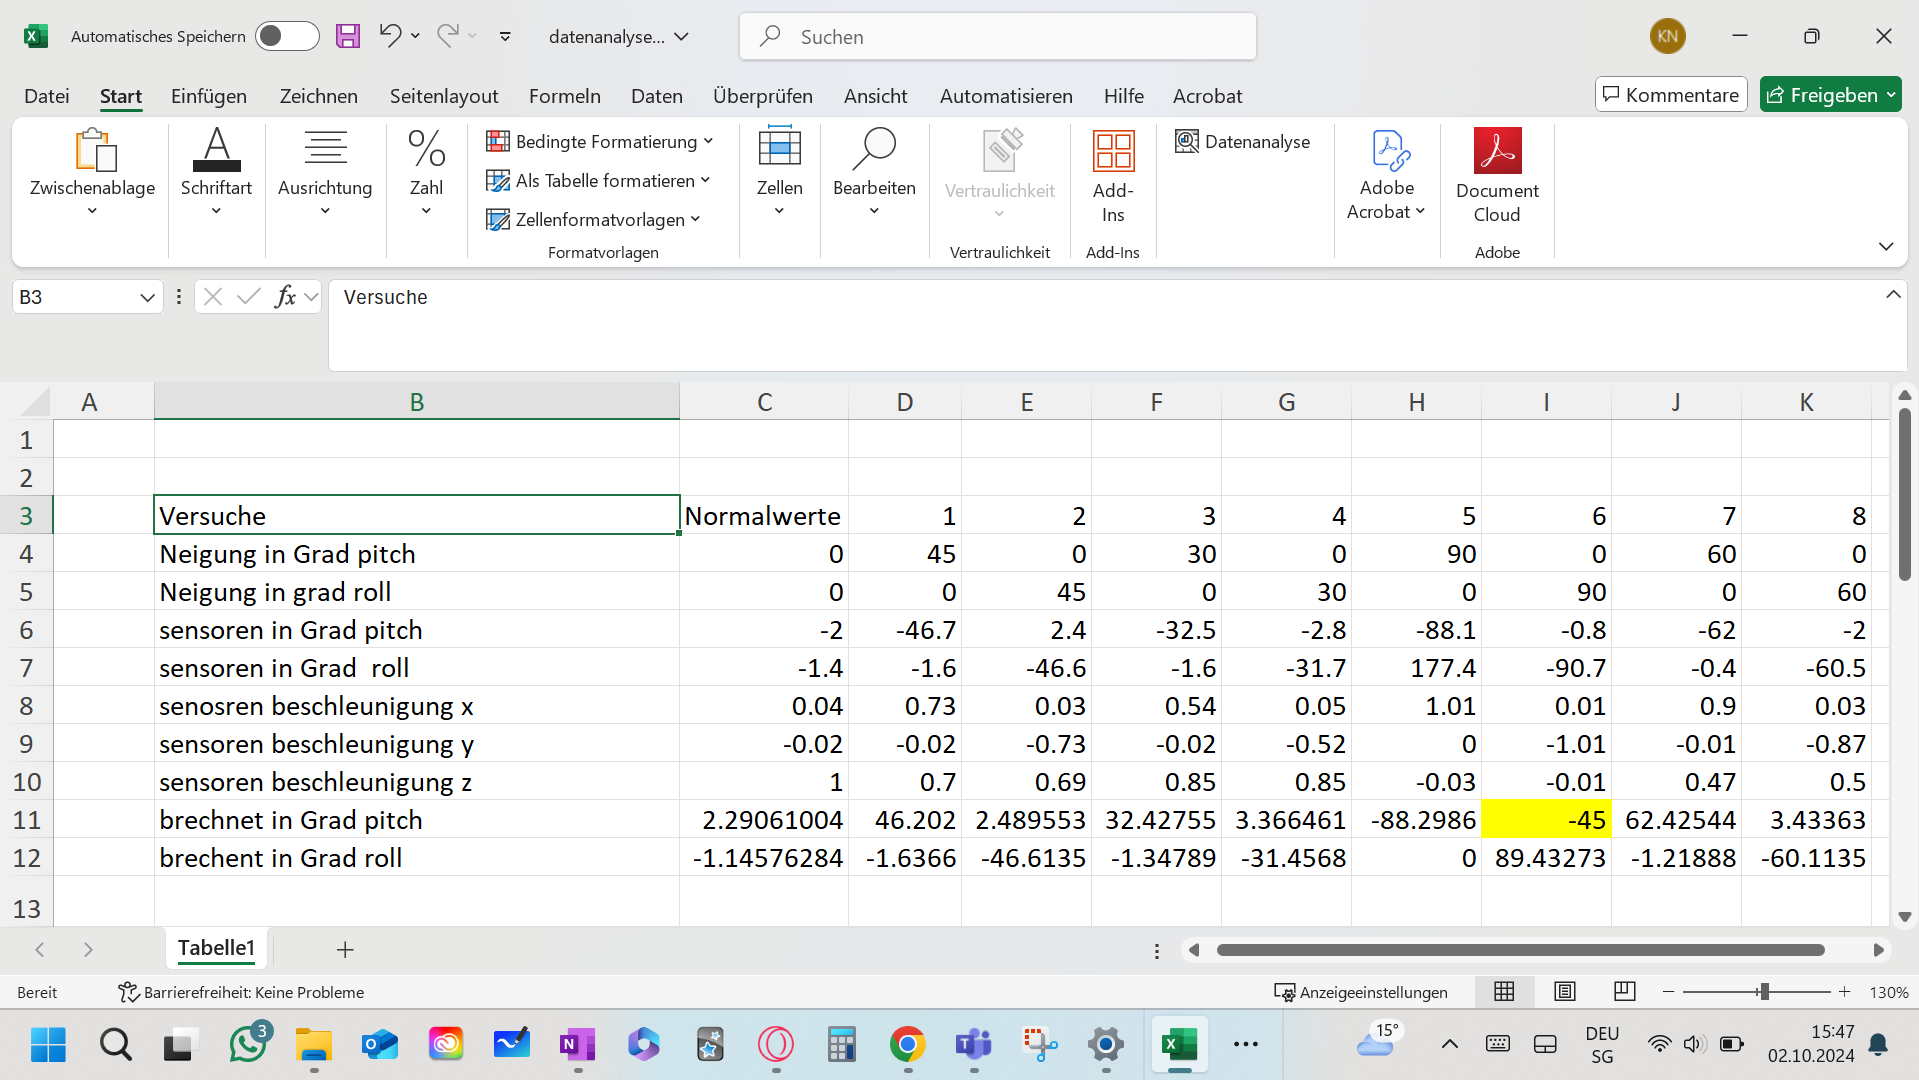
\includegraphics[height=0.3\textheight]{Datenanalyse.png} \vfill
Die ganze Exceltabelle ist auf \href{https://github.com/colordash/Drohne_Project/blob/main/datenanalyse.xlsx}{github} zu finden. 

\subsection{Spalten}
\begin{itemize}
	\item \textbf{Spalte C (Normalwerte)}: Diese Spalte zeigt die theoretischen oder erwarteten „Normalwerte“, also die Werte, die als Standard oder Referenz für die Drohne definiert sind. Diese werden mit den Werten der verschiedenen Versuche (Spalten D bis K) verglichen.
\item\textbf{Spalten D bis K}: Diese Spalten repräsentieren die gemessenen Werte aus acht verschiedenen Versuchen (1 bis 8).
\end{itemize}
\subsection{Zeilen}\begin{itemize}
	\item \textbf{Neigung in Grad pitch (Zeile 4)}: Die Neigung der Drohne in der „Pitch“-Achse, die ihre Vorwärts- oder Rückwärtsneigung beschreibt.
	\item \textbf{Neigung in Grad roll (Zeile 5)}: Die Neigung der Drohne in der „Roll“-Achse, die beschreibt, wie stark die Drohne nach links oder rechts geneigt ist.
	\item \textbf{Sensoren in Grad pitch/roll (Zeilen 6 und 7)}:Diese Zeilen zeigen die gemessenen Daten der Sensoren, die die Neigung in Grad in Pitch (vorwärts/rückwärts) und Roll (links/rechts) erfassen.
	\item \textbf{Sensoren Beschleunigung x/y/z (Zeilen 8 bis 10)}:Diese Zeilen enthalten die gemessenen Beschleunigungswerte der Drohne entlang der drei Achsen (x, y, z), welche die Bewegungen in verschiedene Richtungen anzeigen.
	\item \textbf{Berechnete Werte (Zeilen 11 und 12)}:Die berechneten Winkel in Grad für Pitch und Roll basieren auf den gesammelten Sensordaten. Diese Werte sind das Ergebnis einer mathematischen Berechnung oder Schätzung, die möglicherweise zur Validierung der gemessenen Sensordaten verwendet wird.
	
\end{itemize}

\subsection{Interpretation}\begin{itemize}
	\item {Die Tabelle dokumentiert, wie sich die Drohne in verschiedenen Versuchen verhält, indem Neigungs- und Beschleunigungswerte gemessen und mit Referenzwerten verglichen werden.}
	\item{In den Spalten 1 bis 8 sieht man die Abweichungen der Versuche von den Normalwerten. Einige dieser Werte sind hervorgehoben, was auf besonders signifikante Abweichungen hinweist (z.B. die Messung in Spalte H, Zeile 11 mit einem Wert von -45 Grad Pitch).}
	\item{In Versuchen 1, 2 und 4 scheint die Drohne relativ stabil in ihrer Neigung zu sein, während in anderen Versuchen grössere Abweichungen (wie z.B. in Versuch 6) auftreten.}
\end{itemize}


Die Auswertung der Daten zeigt eine deutliche Reaktion der Sensordaten auf die variierenden Neigungswinkel. Die berechneten Neigungswerte (Pitch und Roll) basieren auf den Messungen der Gyroskope und den Beschleunigungssensoren. Im speziellen Fall von Versuch 6 ist eine signifikante Neigung in der Roll-Achse von 89,43 Grad zu verzeichnen, während der berechnete Pitch-Winkel bei -45 Grad liegt. Solche extremen Abweichungen deuten auf Messfehler hin. Da die Messungen repliziert wurden könnte es an einer potenziellen Instabilität der Drohne liegen. Diese Abweichung müssen genauer untersucht werden, um deren Ursache zu ermitteln.
Die extremen Abweichungen zwischen den geplanten und den berechneten Neigungswerten lassen auf ein Ungleichgewicht in der Stabilisationsregelung der Drohne schliessen. Die Daten deuten darauf hin, dass die Drohne Schwierigkeiten hat, bei solchen extremen Neigungswinkeln stabil zu bleiben.Was durchaus nachvollziehbar ist,. da eine Drohne nicht gebaut ist um in einem 90 Grad picht zu fliegen.



Die Sensordaten der Beschleunigungsmesser zeigen ebenfalls klare Muster in den \(x\)-, \(y\)- und \(z\)-Achsen. Besonders auffällig ist die Verschiebung der \(x\)-Achse in Versuch 6, wo der Wert von 0,01 auf 1,01 ansteigt. Dies signalisiert eine deutliche seitliche Bewegung der Drohne, die im Zusammenhang mit der starken Roll-Neigung steht. Diese Sensordaten sind essenziell, um das Verhalten der Drohne unter verschiedenen Bedingungen zu verstehen.

Die erfassten Beschleunigungswerte ermöglichen es, Rückschlüsse auf die Dynamik der Drohne zu ziehen. In früheren Projekten haben ähnliche Datenmuster gezeigt, dass plötzliche Änderungen der Fluglage und äussere Einflüsse wie Wind die Sensordaten signifikant beeinflussen und eine präzise Abstimmung der Steuerungselemente erforderlich machen.



Die berechneten Neigungswinkel für Pitch\[=ARCTAN(\frac{senosren beschleunigung x}{sensoren\; beschleunigung\; z})*(\frac{360}{2*3.1415926535})\] und Roll\[=ARCTAN(\frac{senosren beschleunigung y}{sensoren\; beschleunigung\; z})*(\frac{360}{2*3.1415926535})\] (siehe Zeilen 11 und 12 der Tabelle) bieten eine wertvolle Vergleichsbasis zu den geplanten Sollwerten. Es zeigt sich, dass die berechneten Werte in einigen Versuchen stark von den vorgesehenen Neigungen abweichen.


In früheren Projekten hat sich gezeigt, dass Abweichungen durch eine Optimierung der Steueralgorithmen und eine präzisere Kalibrierung der Sensoren reduziert werden können. Eine genauere Einstellung der PID-Regler und eine zusätzliche Filterung der Sensordaten könnten in solchen Fällen Abhilfe schaffen.

Das bei Versuch 6 die Werte diese Diskrepanz aufweisen ist schlussendlich, weil eine Drohne nicht gebaut wurde um in einem 90° Grad Pitch zu fliegen und nicht Stabil sein kann.
\end{comment}



\section{Struktur der Firmware}

Betaflight ist dafür konzipiert, Drohnen und Multicopter präzise und reaktionsschnell zu steuern. Es enthält Features wie PID-Regelung, Gyro-Stabilisierung und Flight-Mode-Einstellungen. Betaflight wird auf leistungsfähigen Mikrocontrollern wie STM32F7322 betrieben und bietet umfassende Anpassungsoptionen für die Flugsteuerung.
Weil Betaflight so  Flexibilität und Anpassungsfähig ist nutzt man es vor allem im FPV-Bereich, da es komplexe Flugmanöver und schnelle Reaktionszeiten ermöglicht.

Betaflight ist auf GitHub\cite{GitHubBetaflight} und anderen Repositories in einer klar strukturierten Form verfügbar. Die Hauptordner im Code umfassen:
\begin{itemize}
\item \texttt{src/}: Der wichtigste Ordner, der den Hauptteil des Quellcodes enthält. Hier sind die wesentlichen Module und Implementierungen der Funktionen von Betaflight. 

In diesem Verzeichnis gibt es:
\hspace*{2em}\begin{itemize}\item \texttt{main/}:
Das \texttt{main/} Verzeichnis von Betaflight konzentriert sich auf die Hauptlogik der Firmware, also die Funktionen, die das zentrale Steuerprogramm ausmachen und koordinieren. Eine der wichtigsten Aufgaben des Codes in diesem Verzeichniss ist die Initialisierung des Flugcontrollers. Hier wird der Startprozess ausgeführt, in dem die Sensoren hochgefahren, die Kommunikationsschnittstellen eingerichtet und die Standardflugparameter eingestellt werden. Sobald die Firmware startet, läuft im \texttt{main/} Verzeichnis die Flugsteuerungs- und Kontrolllogik ab, die für das Flugverhalten der Drohne entscheidend ist. Die Algorithmen zur Stabilisierung, insbesondere der PID-Regler, der das Flugverhalten der Drohne in der Luft stabilisiert und anpasst, sind hier ausgeführt. Ausserdem befindet sich hier die Hauptschleife der Firmware, die kontinuierlich in einer Art Endlosschleife abläuft und dabei Eingaben von den Sensoren prüft, Steuerbefehle verarbeitet und Steuerbefehle an die Motoren und Regler weitergibt. Diese Schleife ist für die Reaktionsfähigkeit der Firmware entscheidend und ermöglicht es der Drohne, auf sich verändernde Steuerbefehle blitzschnell und zuverlässig zu reagieren.


\item \texttt{test/}: Das \texttt{test/} Verzeichnis ist ebenfalls ein wesentlicher Bestandteil von Betaflight, da es sicherstellt, dass die Firmware zuverlässig und konsistent auf verschiedenen Plattformen funktioniert. In diesem Verzeichnis sind verschiedene Testarten untergebracht, die dazu beitragen, die Qualität und Stabilität der Software zu gewährleisten. Unit-Tests überprüfen hier die einzelnen Funktionen oder Module isoliert, um sicherzustellen, dass jede Komponente erwartungsgemäss funktioniert. Diese Tests sind besonders wichtig für Kernfunktionen wie mathematische Berechnungen oder die PID-Regelung. Ausserdem gibt es spezielle Hardware-Abstraktions-Tests, die sicherstellen, dass die Firmware mit den unterschiedlichen Prozessoren und Sensoren kompatibel ist, auf denen Betaflight laufen kann. Die Simulationen und Integrationstests gehen noch einen Schritt weiter: Sie lassen die Firmware in einer simulierten Umgebung laufen, sodass das Flugverhalten der Drohne getestet werden kann, ohne eine physische Drohne zu benötigen. Diese Tests überprüfen zudem, ob verschiedene Module und Funktionen der Firmware harmonisch zusammenarbeiten und garantieren so die Integrität des Gesamtsystems.

\end{itemize}
\end{itemize}
	
Die Hauptsteuerungseinheit von Betaflight spielt eine entscheidende Rolle bei der Verarbeitung der Sensor- und Steuerdaten, indem sie Berechnungen zur Flugstabilität durchführt. Um diese Stabilität zu gewährleisten, wird die Steuerung  durch mehrere PID-Controller-Module unterstützt. Betaflight integriert auch Module zur Anbindung an Gyroskop- und Beschleunigungssensoren, die essenziell für die Flugsteuerung sind.

Ein weiterer wichtiger Aspekt der Firmware sind die Mixer-Module, die bestimmen, wie die Eingaben von den Steuerknüppeln der Fernbedienung auf die Motoren verteilt werden. Die Mixer-Formeln variieren je nach Art des Copters, sei es ein Quadcopter, Hexacopter oder ein anderer Typ. Darüber hinaus enthält Betaflight ein Modul, das die Signale von der Fernbedienung empfängt und die entsprechenden Steuerbefehle zur weiteren Verarbeitung weitergibt.


Für die Konfiguration des Flugcontrollers bietet Betaflight ein integriertes Command Line Interface (CLI). Dieses ermöglicht es den Benutzern, bestimmte Parameter direkt über serielle Befehle einzustellen, was eine hohe Flexibilität bei der Anpassung der Firmware an individuelle Bedürfnisse bietet.


Betaflight nutzt \texttt{Makefiles} für den Build-Prozess, um den Code für verschiedene Plattformen und Mikrocontroller-Versionen zu kompilieren. Das Build-System integriert dabei Abhängigkeiten wie \texttt{STM32}-Bibliotheken und spezifische Konfigurationen, die für die jeweilige Hardware benötigt werden. Zudem greift Betaflight auf mehrere externe Bibliotheken zurück, etwa für die Schnittstellensteuerung und zur mathematischen Berechnung von Regelungsalgorithmen. Hierzu gehören auch Bibliotheken wie \texttt{math.h}, die für die Verarbeitung von Flugdaten und die PID-Kontrolle von zentraler Bedeutung sind.

Das PID-Control-Modul ist einer der wichtigsten Teile von Betaflight. Es berechnet kontinuierlich den Unterschied zwischen den Soll- und Ist-Werten (z.B. der aktuellen Position und Orientierung der Drohne) und passt die Motorleistung entsprechend an. Der Code zur PID-Steuerung ist modular und nutzt sowohl die Proportional-, Integral- als auch die Differenzialberechnung für eine präzise Regelung. Der Code für den PID-Regler befindet sich im \texttt{src/main/flight}-Ordner.

\section{Aktuelle Funktionswiese und ursprünglicher Ablauf des Failsafe-Modus}\label{sec:Failsafeablaufalt}

Dieser Abschnitt fokussiert sich auf einen kleinen Teil der gesamten Firmware, genauer gesagt auf die Failsafe-Funktion von Betaflight. Dabei wurden einige Defizite identifiziert, deren Verbesserung den zweiten wesentlichen Bestandteil dieser Arbeit darstellt. Es stellte sich nun die Frage, wie man in die Failsafe-Funktion einen Schalter implementieren, der es der Drohne ermöglicht, aus einer beliebigen Höhe automatisch zu landen. Und wie man die konstante Landung mit der Abhängigkeit des Barometer kontrollieren kann.


Der Failsafe-Modus ist eine von Betaflight bereitgestellte Funktion, die sich über den Betaflight Configurator relativ einfach aktivieren lässt. Dieses Modul stellt sicher, dass die Drohne bei einem möglichen Unterbruch oder einem gestörten Signal der Funkverbindung mit einem definierten und sicheren Ablauf reagiert.

Dieser Ablauf ist in den folgenden zwei Phasen unterteilt:

\subsubsection{Phase 1: Initiale Reaktion}
Sobald die Kommunikation zur Fernbedienung abbricht, wird Phase 1 unverzüglich eingeleitet. Dabei aktiviert die Drohne die zuvor für diesen Fall festgelegten Controller-Werte. Diese Einstellungen bewirken, dass die Drohne für eine bestimmte Zeit in der Luft schwebt, um die Möglichkeit zu schaffen, die Verbindung zur Fernbedienung wiederherzustellen. Die Dauer dieser Phase kann durch die Variable \texttt{failsafe\_delay} definiert werden.

\subsubsection{Phase 2: Endgültige Massnahme}
Wenn die in \texttt{failsafe\_delay} festgelegte Zeit abgelaufen ist, beginnt Phase 2. In dieser Phase stehen drei Prozeduren zur Auswahl:
\begin{itemize}
\item
GPS-Modus:

Diese Option steuert die Drohne mithilfe eines GPS-Moduls zu einem definierten Rückkehrpunkt oder lässt sie an einer sicheren Stelle landen. Da die betrachtete Drohne jedoch kein GPS-Modul besitzt, entfällt diese Möglichkeit.
\item
Drop-It-Modus:

Dies ist der standardmässige Modus, bei dem die Drohne die Motoren sofort abschaltet und unkontrolliert zu Boden fällt. Diese Methode minimiert das Risiko, dass die Drohne unkontrolliert weiterfliegt und dabei Menschen, Tiere oder Objekte gefährdet. Zudem wird verhindert, dass die Drohne in Sperrzonen eindringt und dort Schaden anrichtet.

Der Nachteil dabei ist allerdings, dass der unkontrollierte Absturz, abhängig von der Höhe und dem Untergrund, erhebliche Schäden an der Drohne selbst oder der Umgebung verursachen kann.
\item
Auto-Land-Modus:

In diesem Modus hält die Drohne ihre horizontale Ausrichtung bei und setzt den Gaswert konstant auf den in der Variable \texttt{failsafe\_delay} definierten Wert. Dadurch wird ein kontrolliertes Sinken eingeleitet. Nach Ablauf einer in \texttt{failsafe\_off\_delay} festgelegten Zeit werden die Motoren jedoch ebenfalls abgeschaltet, wodurch die Drohne letztlich zu Boden fällt.
\end{itemize}
\section{Ziel}\label{sec:ziel}
Das Ziel ist es, den Auto-Land-Modus so zu optimieren, dass die Drohne kontrolliert landet und sich erst nach Abschluss der Landung automatisch abschaltet. Dafür soll die Variable \texttt{failsafe\_throttle} kontinuierlich neu berechnet werden. Die Berechnung wird dynamisch auf Grundlage der Abweichung zwischen der angestrebten und der tatsächlich gemessenen Sinkgeschwindigkeit erfolgen. Zusätzlich sollte der Bodenkontakt erkannt werden, woraufhin sich die Drohne automatisch abschalten soll.
 

\section{Versuche}\label{sec:tests}
zu Beginn der Codeanalyse wurden verschiedene Teile des Quellcodes auf ihre Auswirkungen auf ihre Flugeigenschaften der Drohe untersucht. Dazu wurden verschiedene Funktionen gezielt deaktiviert und das Flugverhalten der Drohen mit dem geänderten Programm analysiert. Dies erfolgte ausgehend vom \texttt{src/main/flight/mixer\textunderscore init.c/}. 

In diesem Versuch wurden die Zeilen 82 - 241, die für die Initialisierung anderer Drohnentypen zuständig sind deaktiviert. Nach der Durchführung von verschiedenen Tests mit dem neuen Code auf der Drohe konnte die Richtigkeit dieser Annahme aufgrund der Analyse bestätigt werden

An diesem Stand der Arbeit hatten wir noch nicht das profunde Wissen von jetzt und zudem waren wir am Beginn des erlernen der Codesprache C. 

Danach kam die \texttt{const mixer\textunderscore t mixers[] = \{...\}} Fukntion. Die Struktur der Funktion im \texttt{mixers[]}-Array besteht aus drei Komponenten:
\begin{itemize}
\item 
Anzahl der Motoren
\item  
Booleschen Wert\cite{boolsch} für die Verwendung von Servos 
\item  
Zeiger auf die jeweilige Mixer-Funktion. 
\end{itemize}
Im Beispiel \texttt{\{0, false, NULL\}} beschreibt der Eintrag eine Konfiguration ohne Motoren (Wert 0), ohne die Nutzung von Servos (\texttt{false}), und ohne eine spezifische Mixer-Funktion (durch \texttt{NULL} gekennzeichnet). Dieser Eintrag könnte als Platzhalter oder als Standardwert verwendet werden, wenn keine aktive Mixer-Konfiguration erforderlich ist. 

Darauf folgten viele weitere Versuche, die hier nicht weiter erläutert werden.

\section{Titel unbekannt}
Nachdem ein grundlegendes Verständnis für die verwendete Programmiersprache und deren spezifische Anwendung in diesem Kontext erlangt wurde, begann der schrittweise Weg zur Annäherung an das gesetzte Ziel. Für das Verständnis, wie die Failsafe-Funktion programmiert wurde, erwiesen sich die Dateien failsafe.h und failsafe.c als besonders hilfreich. In diesen Dateien werden alle wichtigen Parameter innerhalb einer zentralen Datenstruktur definiert. Dadurch besteht nun die Möglichkeit, diese Parameter direkt und dauerhaft im Quellcode der Firmware festzulegen, sodass eine nachträgliche Bearbeitung über die Applikation Betaflight Configurator nicht mehr erforderlich ist. \footnote{Alle in diesem Kapitel erwähnten Quellcodes sind in unserem GitHub-Repository in umfangreicherer Form verfügbar.\cite{GitHub}} 
\lstinputlisting[
label=lst:Standardwerte_failsafe,
caption={Standardwerte vom Failsafecode},
]{code/Standardwerte_failsafe.c}


Um die definierten Ziele zu erreichen, soll die Variable \texttt{failsafe\_throttle} dynamisch neu berechnet werden. Daher war es zunächst erforderlich, zu überprüfen, an welcher Stelle der Wert von \texttt{failsafe\_throttle} an den ESC übergeben wird. Schnell wurde klar, dass dies nicht in der Datei \texttt{failsafe.c} geschieht. Nach einiger Analyse konnte in der Datei \texttt{mixer.c} eine sehr relevante Funktion identifiziert werden.

\lstinputlisting[
label=lst:applyMixToMotors,
caption={[applyMixToMotors]applyMixToMotors Funktion in \texttt{mixer.c}},
]{code/applyMixToMotors.c}


Diese Funktion steuert die Motoren einer Drohne, indem sie den gewünschten Schub (Throttle) und die Roll-, Nick- und Gier-Werte (Motor-Mix) kombiniert. Für jeden Motor wird der Ausgangswert berechnet, indem der Schub mit einem Mischungsfaktor (aus dem aktiven Mixer) skaliert wird. Optional wird der Motoroutput durch Thrust-Linearization angepasst, um eine bessere Ansprechkurve der Motoren zu erreichen. Falls Failsafe aktiv ist, wird der Motoroutput auf einen sicheren Bereich begrenzt, insbesondere für das DSHOT-Protokoll\footnote{Das DShot-Protokoll ist ein digitales Steuerprotokoll, das Motorbefehle präziser und störungsresistenter übermittelt als analoge Verfahren wie Pulsweitenmodulation. Es arbeitet ohne Kalibrierung und ermöglicht eine Rückmeldung, beispielsweise zur Erfassung der Motordrehzahl.}, um spezielle reservierte Werte zu vermeiden. Ohne Failsafe wird der Motoroutput lediglich auf ein Minimum und Maximum beschränkt. Wenn die Drohne nicht scharfgeschaltet\footnote{Das Scharfstellen (auch "Armen") einer Drohne bezeichnet den Vorgang, bei dem die Drohne in den Flugmodus versetzt wird und die Motoren startbereit gemacht werden. Dieser Prozess ist aus Sicherheitsgründen erforderlich, um ungewolltes Starten zu verhindern.} ist, wird jeder Motor auf den Wert für den deaktivierten Zustand gesetzt.

Besonders spannend erscheint die Zeile 23, in der der \texttt{motorOutput} definiert wurde. Es schien naheliegend, den \texttt{motorOutput} direkt zu manipulieren und ihn an gewünschte Werte anzupassen – zumindest nach erster Überlegung. Daher wurde der \texttt{motorOutput} statisch auf den Wert 1200 gesetzt, da \texttt{failsafe\_throttle} denselben Wert besitzt und wir waren sicher, dass dies funktionieren würde. Doch nach dem Kompilieren und Flashen der Firmware zeigte sich ein anderes Ergebnis. Bei manuellem Aktivieren des Failsafe-Modus führte die Drohne einen Vorwärtssalto aus und stellte wenige Augenblicke später den Betrieb vollständig ein. Vermutlich lag die Ursache dieses Verhaltens im Wert von \texttt{motorOutput}, der in einen für das DSHOT-Protokoll reservierten Bereich gelangte. Infolgedessen deaktivierte sich die Drohne aus Sicherheitsgründen selbst.

Die Entscheidung, \texttt{motorOutput} an dieser Stelle zu manipulieren, erwies sich als problematisch, da diese Variable nicht nur den Throttle-Wert enthält, sondern auch Roll- und Nick-Werte integriert. Diese Werte werden kombiniert, um den spezifischen Output für jeden Motor zu berechnen. Ein in diesem Versuch angewandtes Vorgehen führte dazu, dass die Drohne nicht mehr in der Lage war, sich selbstständig auszubalancieren und stabil an Ort und Stelle zu bleiben.

\section{Finales Produkt}
Nach diesem Fehlschlag wurde deutlich, dass dieser Parameter an einer anderen Stelle definiert wird. Nach weiterer Analyse der Fukntionen stiess man bald auf die Dateien \texttt{rx.c} und \texttt{rx.h}. „RX“ steht für „Receiver“ und umfasst die Dateien, die unter anderem die Kommunikation zwischen der Drohne und der Fernbedienung steuern. In diesen Dateien fand sich eine weitere zentrale Funktion:

\lstinputlisting[
label=lst:detectAndApplySignalLossBehaviour,
caption={[DetectAndApplySignalLossBehaviour]Zentrale Funktion der Throttle-Steuerung bei einem Failsafe.},
]{code/detectAndApplySignalLossBehaviour.c}

Die Funktion \texttt{detectAndApplySignalLossBehaviour} steuert, wie die Drohne auf Signalverlust reagiert. Wenn der Failsafe-Modus aktiviert ist (d.h., \texttt{failsafeIsActive()} ist wahr), werden ungültige RC-Signale durch Failsafe-Werte ersetzt. Besonders der Throttle-Kanal wird auf einen sicheren Failsafe-Wert gesetzt, um die Drohne kontrolliert zu halten. Für andere Kanäle wird der Wert auf den mittleren Wert gesetzt. Wenn der Failsafe-Modus Phase 2 erreicht, sorgt die Funktion dafür, dass die Drohne weiterhin stabil fliegt und sich sicher landen kann, selbst wenn das Signal verloren geht. Sie überprüft regelmässig, ob die Drohne gültige Daten empfängt und passt die Steuerung entsprechend an. Zusätzlich werden mit den Funktionen \texttt{failsafeOnValidDataReceived()} oder \texttt{failsafeOnValidDataF\-ailed()} Timer gestartet, die den Übergang zwischen den verschiedenen Failsafe-Phasen steuern.


In der für diese Arbeit entscheidenden Zeile 28 wurde der Wert von sample auf einen konstanten Wert, wie zum Beispiel 1000, gesetzt. Im Vergleich zum vorherigen Versuch zeigte die Drohne ein völlig anderes Verhalten. Sie glitt relativ kontrolliert in Richtung Boden, jedoch etwas zu schnell, da der sample-Wert zu niedrig war. Durch die Erweiterung dieses Code-Schnipsels und weitere praktische Tests wurde klar, dass diese Funktion etwa 5000 Mal pro Sekunde ausgeführt wird und Änderungen des sample-Werts an den ESC weiterleitet. Daraus ergab sich, dass dieser Punkt der ideale Ort für die Implementierung der zusätzlichen Failsafe-Modus-Funktion war. In der Folge wurde ein relativ einfacher Steuermechanismus für den Throttle-Wert in die Datei \texttt{rx.c} integriert. 

\lstinputlisting[
label=lst:throttle_steuerung,
caption={[Berechnung des Throttle-Wertes] Eigens programmierte Funktion zur Berechnung des Throttle-Wertes},
]{code/throttle_steuerung.c}


Diese Funktion berechnet den Throttle-Wert dynamisch und gibt ihn zurück, wodurch sie anstelle eines festen Wertes verwendet werden kann. Der Code ermittelt den Failsafe-Throttle-Wert, der zum Einsatz kommt, wenn die Drohne in den Failsafe-Modus wechselt. Zu Beginn wird der Failsafe aktiviert, und der Startwert für den Throttle sowie die Starthöhe werden festgelegt. Der Throttle-Wert wird dann alle 100 Millisekunden aktualisiert und neu berechnet, basierend auf der Höhenänderung der Drohne. Dieser Zeitintervall kann durch den Parameter, der der Funktion beim Aufruf übergeben wird, sehr präzise gesteuert werden. Wenn die Drohne steigt (d.h., die Höhe nimmt zu), wird der Throttle-Wert um einen festen Betrag verringert, um die Drohne langsamer sinken zu lassen. Wenn die Drohne jedoch zu schnell sinkt (mehr als 0,2 Meter pro Sekunde), wird der Throttle-Wert erhöht, um einen sicheren Sinkflug zu gewährleisten. Wenn die Höhe stabil bleibt, bleibt der Throttle-Wert unverändert.

Zusätzlich wird der Throttle-Wert auf ein Minimum von 1000 und ein Maximum von 1400 begrenzt, um sicherzustellen, dass der Throttle-Wert innerhalb eines sicheren Bereichs bleibt. Der Code sorgt somit dafür, dass die Drohne im Failsafe-Modus kontrolliert bleibt und nicht zu schnell sinkt.


\begin{comment}
\subsection{Failsafe-Unfall}
Im Rahmen des Experiments wurde zunächst die Failsafe-Funktion in der Steuerungssoftware der Drohne programmiert. Dabei wurde der Code so angepasst, dass die Drohne im Falle eines Kommunikationsverlusts zwischen Fernbedienung und Drohne in einen sicheren Zustand übergeht. Zwei Modi wurden hierbei definiert:  
\begin{itemize}
	\item Modus 2: Die Drohne landet kontrolliert.  
	\item Modus 1: Die Drohne kehrt in einen Flugzustand zurück und hält ihre Höhe.  
\end{itemize}
Um die Failsafe-Funktion zu testen, wurde der Kommunikationsverlust simuliert, indem die Fernbedienung während des Fluges ausgeschaltet wurde. Dies sollte die Drohne gemäss der programmierten Logik in Modus 2 (Landung) versetzen.

Entgegen den Erwartungen zeigte die Drohne ein inkonsistentes Verhalten. Anstatt kontrolliert zu landen, wechselte sie zunächst in Modus 2, ging danach jedoch in Modus 1 über und begann erneut zu fliegen. Diese fehlerhafte Sequenz führte dazu, dass die Drohne die Kontrolle verlor, gegen eine Wand flog und dabei die Propeller beschädigt wurden.  

Die unerwartete Umschaltung zwischen den Modi offenbarte eine kritische Schwachstelle im programmierten Code. Eine detaillierte Analyse ergab, dass die Bedingungen für den Moduswechsel nicht eindeutig definiert waren, wodurch der Wechsel von Modus 2 zu Modus 1 unbeabsichtigt ausgelöst wurde.

Das Experiment zeigte, dass die ursprüngliche Implementierung der Failsafe-Funktion nicht den Anforderungen einer sicheren und zuverlässigen Steuerung entsprach. Der fehlerhafte Ablauf führte zu einem gefährlichen Szenario, das die Wichtigkeit einer präzisen Programmierung und gründlichen Überprüfung der Steuerungssoftware unterstreicht.  

Die Beobachtungen verdeutlichten, dass die Logik des Moduswechsels überarbeitet werden musste, um sicherzustellen, dass die Drohne nach Verlust der Verbindung ausschliesslich in Modus 2 verbleibt, bis sie sicher gelandet ist.  

Das Experiment zeigte Schwachstellen in der Umsetzung der Failsafe-Funktion auf und lieferte wertvolle Erkenntnisse für die Verbesserung der Software. Die notwendigen Korrekturen im Code wurden durchgeführt, und die Logik des Moduswechsels wurde so angepasst, dass eine erneute Umschaltung in Modus 1 ausgeschlossen ist. In zukünftigen Tests wird der Fokus auf eine umfangreiche Simulation und Prüfung der Sicherheitsfunktionen gelegt, um ähnliche Fehlverhalten zu vermeiden.  
\end{comment}

\section{Fazit}\label{sec:Fazit6}
\begin{comment}
%zu sehr Zusammenfassung für mich sorry
In diesem Kapitel wird der Weg beschrieben, wie der Auto-Land-Modus der Drohne verbessert wurde, sodass sie kontrolliert landet und sich nach der Landung abschaltet. Am Anfang standen einfache Versuche, bei denen vor allem nach Gefühl vorgegangen wurde, weil das Verständnis für die Programmiersprache C noch fehlte. Schritt für Schritt wurden verschiedene Dateien wie mixer.c, failsafe.c und rx.c untersucht, um herauszufinden, wo und wie der entscheidende Throttle-Wert für den Failsafe-Modus berechnet wird.

Ein erster Ansatz, den Motoroutput direkt zu manipulieren, führte zu einem unerwarteten Fehlschlag: Die Drohne machte einen Vorwärtssalto und schaltete sich ab. Das Problem war, dass der Motoroutput nicht nur den Throttle-Wert, sondern auch Steuerwerte wie Roll und Nick enthält. Dadurch wurde die Drohne instabil.

Nach diesem Rückschlag konzentrierte sich die Arbeit auf die Dateien rx.c und rx.h, die die Kommunikation mit der Fernbedienung steuern. Dort wurde schliesslich die Funktion gefunden, die den Failsafe-Modus steuert. Durch Anpassung des Throttle-Werts in dieser Funktion und viele Tests konnte ein kontrolliertes Sinken der Drohne erreicht werden. Die Drohne landete am Ende zuverlässig und sicher, wodurch das gesetzte Ziel zumindest teilweise erfolgreich erreicht wurde.
\end{comment}


Man sieht, dass durch gezielte Programmierung und Tests die Funktionsweise des Failsafe-Modus in Betaflight optimiert werden konnte. Insbesondere die Entwicklung einer dynamischen Berechnung des Failsafe-Throttle-Werts ermöglichte einen kontrollierten Sinkflug der Drohne. Die vorgenommenen Änderungen an der Firmware, insbesondere die Implementierung der neuen Steuerlogik und die Berücksichtigung der Höhenänderung, führten zu einer präziseren und zuverlässigen Steuerung während des Failsafe-Modus. 

Dennoch treten in der Praxis weiterhin Fehler auf. Der Barometer ist ein sehr empfindlicher Sensor und reagiert stark auf Wind. Dadurch hat er Schwierigkeiten, die tatsächliche Sinkgeschwindigkeit in Bodennähe präzise zu erfassen, da die Drohne dort durch ihre Rotoren einen starken Eigenwind erzeugt. Zudem kann die Drohne nicht stabil auf einer Position schweben, sondern weist immer eine leichte Abdrift auf. Dieser Abdrift summiert sich während des Auto-Land-Modus zunehmend, wodurch die Drohne unerwartet weit in seitliche Richtungen abdriften kann. Diese Probleme konnten im Rahmen dieser Arbeit nicht vollständig gelöst werden, jedoch wurde überlegt wie man diese Probleme beheben könnte (siehe \hyperref[sec:ausblick]{7.6.2 Ausblick}).\label{probleme}

Die praktischen Tests und Codeanalysen zeigten, wie wichtig eine detaillierte Untersuchung der Code-Logik und der verschiedenen Module für die Optimierung der Firmware ist. Fehler wie der unkontrollierte Vorwärtssalto beim ersten Versuch verdeutlichten die Notwendigkeit, den Throttle-Wert nicht isoliert zu betrachten, sondern im Kontext der gesamten Flugstabilität und Steuerlogik.

Insgesamt wurde durch diesen Prozess nicht nur die Funktionsweise des Failsafe-Modus verbessert, sondern auch ein tieferes Verständnis für die Softwarestruktur von Betaflight und die Interaktion der verschiedenen Firmware-Module gewonnen. 












	
\chapter{Resultate} \label{ch:Resultate}

In diesem Kapitel werden die Ergebnisse des Projekts reflektiert, was die Programmierung und den Zusammenbau der Drohne angeht.  
\begin{comment}
\section{Datenanalyse und -verarbeitung}
Die Datenerfassung bildete einen zentralen Bestandteil des Projekts, um die genaue Fluglage der Drohne während der verschiedenen Testversuche zu analysieren.
\subsection{Datenerfassung}  
 Hierzu wurden kontinuierlich Beschleunigungsdaten vom Accelerometer aufgezeichnet und in Echtzeit in Winkel umgerechnet. Die von der Software Betaflight Configurator bereitgestellten Daten dienten dabei nicht nur der Visualisierung der Neigung der Drohne in Form einer 3D-Grafik, sondern auch als Grundlage für weitere Berechnungen. Neben den berechneten Winkelwerten konnten auch die Rohdaten des Accelerometers extrahiert werden, was eine detaillierte Untersuchung der Neigungswinkel entlang der Längs- und Querachse ermöglichte. Um die Präzision der Messungen sicherzustellen, wurden die Sensoren vor Beginn der Tests sorgfältig kalibriert. Besonderes Augenmerk wurde auf die Wiederholbarkeit und Reproduzierbarkeit der Messungen gelegt, wodurch die allgemeine Gültigkeit der Ergebnisse gewährleistet wurde. Zusätzlich wurden alle Werte, soweit sinnvoll, auf zwei Dezimalstellen gerundet, um eine ausreichende Genauigkeit sicherzustellen.

\subsection{Datenanalyse}  
Die gesammelten Daten wurden sorgfältig analysiert, um mögliche Muster oder Auffälligkeiten zu identifizieren. Dabei lag der Fokus auf der Interpretation der Accelerometer-Rohdaten sowie der daraus berechneten Winkelwerte. Verschiedene statistische Methoden und visuelle Analysen wurden verwendet, um Trends und Korrelationen zu untersuchen. Durch diese systematische Auswertung konnten präzise Rückschlüsse auf die Leistung und Stabilität der Drohne gezogen werden. Die Analyse lieferte wertvolle Einblicke in die Funktionsweise der Sensoren und ihrer Kalibrierung, was entscheidend für die Arbeit war.

\subsection{Ergebnisse}  
Im Rahmen der Datenanalyse wurden anfänglich auffällige Muster in den Ergebnissen entdeckt, die zunächst unverständlich erschienen. Diese Auffälligkeiten waren besonders irritierend, da die verwendete Open-Source-Software von einer grossen Anzahl von Nutzern verwendet wird und keine ähnlichen Probleme berichtet wurden. Nach einer gründlichen Überprüfung wurde festgestellt, dass die Ursache dieser Muster in einer fehlerhaften Berechnung lag. Nachdem die Berechnungen angepasst und verbessert wurden, konnten keine weiteren Anomalien festgestellt werden. Mit der korrigierten Analyse verliefen alle weiteren Tests wie erwartet, und die Drohne zeigte die erwartete Stabilität und Leistung.


\subsection{Datenerfassung}
Wie wurden die Daten erfasst und waren sie entsprechend unseren Erwartungen? 

Zur Ermittlung der genauen Fluglage der Drohne während der verschiedenen Testversuche am Boden wurden Beschleunigungsdaten vom Accelerometer kontinuierlich aufgezeichnet und in Echtzeit in Winkel umgerechnet. Diese Winkelwerte werden unter anderem direkt von der von uns verwendeten Software "Betaflight Configurator" berechnet und mit einer anschaulichen 3D-Grafik ausgegeben. Diese Daten geben Auskunft über die Neigung der Drohne um die Längs- und Querachse (Pitch und Roll). Zudem gibt die bereits erwähnte Software die Rohdaten des Accelerometers aus. Diese sind essenziell für weitere Berechnungen, in denen die Neigung der Drohne entlang der Längs- und Querachse ausschliesslich anhand der Beschleunigungsdaten selbst berechnet wurde. Somit umfassen die erfassten Daten sowohl die Rohdaten der Sensoren als auch die daraus berechneten Winkelwerte. 
Vor der Durchführung der Messungen wurden die Sensoren neu kalibriert, um Abweichungen zu minimieren. Bei der Durchführung der Messungen wurde besonders auf Wiederholbarkeit und Reproduzierbarkeit geachtet, um die allgemeine Gültigkeit der Ergebnisse zu gewährleisten. Um die Genauigkeit zu erhöhen, wurden alle Daten und Ergebnisse, wo möglich, auf zwei Nachkommastellen gerundet. 

\subsection{Datenanalyse}
Wie wurden die gesammelten Daten analysiert, um Muster zu erkennen?


\subsection{Ergebnisse}
Wurden auffällige Datenmuster identifiziert? Was wurde herausgefunden? 

Wider erwarten wurde ein auffälliges Datenmuster festgestellt. Dies war sehr irritierend, da tausende diese Open-Source-Software benutzen. Später haben wir festgestellt, dass diese Auffälligkeit an unserer Berechnung lag und mit der neuen verbesserten Rechnung wurden keine auffälligen Datenmuster mehr erkannt und alles lief wie es sollte.
\end{comment}
\section{Technische Ergebnisse}

\subsection{Erfolgreiche Implementierungen}
Der von Betaflight bereitgestellte Quellcode konnte nach umfangreicher Recherche und zahlreichen Versuchen zu einer für die Drohne verständlichen Hex-Datei kompiliert werden. Wegweisend hierfür war die Anleitung von Betaflight, die detailliert beschreibt, wie dieser Prozess erfolgreich durchzuführen ist. Die einzelnen Arbeitsschritte wurden dokumentiert und sind in unserem Git-Repository ausführlich beschrieben (siehe Fussnote).

Nach anfänglichen Schwierigkeiten gelang es schliesslich, die selbst generierte Firmware auf die Drohne zu flashen. Dieser Vorgang erfolgte über die Betaflight Configurator-App im sogenannten DFU-Mode. Der DFU-Mode (Device Firmware Upgrade Mode) ist ein spezieller Betriebsmodus von Mikrocontrollern (MCUs), der es ermöglicht, Firmware direkt über eine USB- oder serielle Verbindung zu aktualisieren, ohne dass ein externer Programmieradapter erforderlich ist. Da Windows den hierfür benötigten Treiber standardmässig nicht unterstützt, musste dieser mithilfe einer externen Applikation manuell installiert und der zuvor verwendete Treiber überschrieben werden (siehe Fussnote).

Der gesamte Prozess, eine eigene Version des Quellcodes zu erstellen und erfolgreich auf die Drohne zu flashen, war zwar langwierig, brachte uns jedoch wertvolle Erkenntnisse und ein hohes Mass an Flexibilität, zur späteren Weiterentwicklung des Quellcodes. Der Zugewinn an praktischer Erfahrung und tiefem Verständnis für den Entwicklungsprozess war für uns auch ein zentraler Teil dieser Arbeit.

\subsection{Funktionalität der Drohne}
Das wichtigste Kriterium konnte erfüllt werden, die Drohne fliegt einwandfrei am Ende dieser Arbeit. Dank des öffentlich verfügbaren Quellcodes von Betaflight fliegt die Drohne sehr stabil und reagiert schnell auf Eingaben über die Fernbedienung. Der erfolgreiche Betrieb ist jedoch vor allem auf die präzise ausgewählten und optimal aufeinander abgestimmten Bauteile zurückzuführen. Diese wurden korrekt und stabil miteinander verbunden, was eine fehlerfreie Funktion ermöglicht. Abschliessend wurden über die Betaflight Configurator-App die finale Konfigurationen vorgenommen, um die korrekte Funktionsweise sicherzustellen. Dank dieses sorgfältig durchgeführten Arbeitsprozesses fliegt die Drohne im normalen Flugmodus äusserst stabil und präzise. 

Die in dieser Arbeit weiterentwickelte Failsafe-Funktion funktioniert grundsätzlich, und die Drohne beginnt kontrolliert zu sinken. Der selbst entwickelte Teil des Quellcodes konnte zudem erfolgreich implementiert und kompiliert werden. 
Dennoch traten während der praktischen Tests unerwartete Probleme auf. Das erste Problem ist das Abdriften der Drohne: 

Nach kurzer Zeit beginnt die Drohne ohne korrigierende Eingaben horizontal in eine Richtung zu driften. Dieses Probleme konnte, wie schon \hyperref[probleme]{zuvor} erwähnt, im Rahmen dieser Arbeit nicht gelöst werden. Es wurde jedoch \hyperref[sec:ausblick]{erörtert}, wie eine Lösung für diese Probleme aussehen könnte.


Das zweite Problem betrifft die Annäherung an den Boden:

Wenn die Drohne nahe am Boden schwebt, erzeugen die Rotoren starke Eigenwinde, die den empfindlichen Barometer erheblich beeinflussen und fehlerhafte Werte liefern können. Dadurch landet die Drohne nicht vollständig, sondern schwebt wenige Zentimeter über dem Boden. Trotz dieser Bedenken kann man sagen, dass die Funktionalität grösstenteils gewährleistet ist.

\subsection{Probleme und Lösungsansätze}
%Welche technischen Schwierigkeiten traten auf, z. B. beim Zusammenbau oder der Programmierung? Wie wurden diese behoben?

Die zuvor erwähnten technischen Schwierigkeiten treten weiterhin auf. Das Abdriften lässt sich dadurch erklären, wie die Drohne ihre Balance hält. Sie versucht, sich stets waagerecht auszurichten, wenn keine anderen Steuerbefehle für Neigung und Roll gegeben werden, was während des Failsafe-Modus der Fall ist. Die ursprüngliche Kalibrierung der \hyperref[sec:IMU]{IMU} ist jedoch nicht perfekt, weshalb die Drohne nicht exakt waagerecht ausgerichtet ist – eine technische Herausforderung, die sich nicht vollständig lösen lässt. Eine hilfreiche Massnahme kann die Trimmfunktion an der Fernbedienung sein. Doch selbst mit dieser Methode bleibt ein kleiner Fehler bestehen, der zu einem Abdriften in eine Richtung führt. Dieses Problem könnte durch das Hinzufügen eines GPS-Moduls behoben werden. Ein solches Modul würde der Drohne ermöglichen, Abweichungen von ihrer ursprünglichen Position zu erkennen und entsprechend zu korrigieren.

Das zweite Problem, dass die Drohne durch den von ihr selbst erzeugten Wind abgelenkt wird und dadurch nicht vollständig landen kann, könnte durch den Einsatz eines zusätzlichen Sensors gelöst werden. Statt sich ausschliesslich auf die Messwerte des Barometers zu stützen, wäre es sinnvoll, auch das Integral der Beschleunigungsdaten zu verwenden. Dies würde die Geschwindigkeitsberechnung präzisieren und den Algorithmus insgesamt verbessern. 

\section{Erreichte Ziele und Abweichungen}

\subsection{Zielerreichung}
%Wurden die Projektziele grösstenteils erreicht? Welche Ziele waren zu ambitioniert und mussten angepasst werden oder konnten nicht erfüllt werden?


Die in dieser Arbeit gesteckten Ziele konnten weitgehend erfolgreich erreicht werden. Das übergeordnete Ziel, eine Drohne zu entwickeln, die mithilfe eines Schalters aus beliebiger Höhe automatisch landen kann, wurde durch die Implementierung der entsprechenden Fluglogik und des Failsafe-Modus realisiert.

Die Auswahl und der Zusammenbau der Hardwarekomponenten wurden erfolgreich abgeschlossen. Die sorgfältig ausgewählten Flugcontroller, Motoren, Sensoren und Akkus erwiesen sich als geeignet, um die Stabilität und Leistung der Drohne zu gewährleisten. Der Zusammenbau, einschliesslich der Installation von Motoren, Propellern und Sensoren sowie der Verkabelung, verlief planmässig. Die abschliessenden Tests bestätigten die einwandfreie Funktion der Hardware und bildeten die Grundlage für die Implementierung des Landeschalters.

Die Landeschalter-Funktion wurde erfolgreich programmiert. Nach einer gründlichen Analyse des Betaflight-Sourcecodes konnte die Steuerlogik identifiziert und durch spezifische Anpassungen erweitert werden, um die automatische Landefunktion zu realisieren.
Die implementierten Algorithmen ermöglichen der Drohne, beim Aktivieren des Landeschalters eine kontrollierte Sinkgeschwindigkeit einzuhalten. Insbesondere die Integration der Barometerdaten für die Überwachung der Sinkgeschwindigkeit erwies sich als entscheidend für den Erfolg.
Die Funktionalität wurde in verschiedenen Testszenarien geprüft. Dabei zeigte sich, dass die Drohne auf Steuerbefehle korrekt reagiert und eine stabile Landung gewährleistet. Trotz herausfordernder Bedingungen, wie Wind oder Abdrift während des Auto-Land-Modus, bewies die Funktion eine hohe Zuverlässigkeit. 





%Die Projektziele wurden insgesamt erreicht, obwohl die anfänglichen Ambitionen das tatsächliche Arbeitspensum und die technische Komplexität unterschätzt hatten. Ursprünglich war geplant, eine Drohne mit umfangreichen Funktionen zu entwickeln, die auf fortgeschrittenen Mechanismen und Algorithmen basiert. Jedoch stellte sich heraus, dass die geplanten Funktionen für die verfügbare Zeit und Ressourcen zu anspruchsvoll waren. Nach einer Anpassung der Zielsetzungen konnte die Drohne erfolgreich aufgebaut, programmiert und getestet werden.

\subsection{Abweichungen vom Plan}
%Gab es signifikante Abweichungen vom ursprünglichen Plan aufgrund unerwarteter Hindernisse? Was wurde umgeplant?

Im Verlauf des Projekts gab es signifikante Abweichungen vom ursprünglichen Plan, insbesondere in Bezug auf die Softwareentwicklung. Der Quellcode der Drohne erforderte eine eingehende Analyse und ein umfangreiches Verständnis, was deutlich mehr Zeit in Anspruch nahm als ursprünglich erwartet. Diese unerwartete Komplexität führte dazu, dass einige der ursprünglich angedachten Funktionen gestrichen oder vereinfacht wurden.
\section{Unerwartete Herausforderungen}

\subsection{Technische Herausforderungen}
%Welche unerwarteten technischen Probleme traten auf, z. B. Kompilierungs- und Kommunikationsfehler zwischen der Drohne und der Fernbedienung?

Während der Entwicklung und Umsetzung des Projekts traten verschiedene technische Probleme auf, die teilweise erheblichen Mehraufwand und Verzögerungen verursachten.   

Eines der zentralen Hindernisse war die Kompatibilität zwischen verschiedenen Software-Versionen. Eine der verwendeten Abhängigkeiten war nicht aufeinander abgestimmt, was dazu führte, dass bestimmte Funktionen nicht wie erwartet arbeiteten. Dies erforderte umfangreiche Anpassungen und die Versionsanpassung, um die Kompatibilität herzustellen.  
 
Durch die Zusammenarbeit im Team kam es bei der Versionsverwaltung mit Git zu Konflikten während der Merge-Prozesse. Besonders komplexe Änderungen am selben Kapitel der Arbeit führten zu Inkonsistenzen im Code, die manuell aufgelöst werden mussten. Dies erforderte zusätzliche Abstimmungen im Team und kostete wertvolle Entwicklungszeit. Doch am Schluss hat gab es immer eine gute Lösung

Während der Entwicklungsphase waren längere Ladezeiten ein unerwartetes Hindernis. Besonders beim Kompilieren des Codes oder beim Testen der Firmware führte dies zu Verzögerungen im Workflow. Um dies zu minimieren, mussten andere Geräte benutzt werden um die Effizienz zu steigern.  

Ein scheinbar kleiner, aber extrem zeitintensiver Fehler war ein Syntaxfehler in der Bibliotheksdatei. Ein vergessenes Komma sorgte dafür, dass der Code nicht ausführbar war und TeXstudio das Dokument nicht kompilieren konnte. Die Fehlersuche war äusserst aufwendig, da der Fehler erst nach längerer Analyse gefunden wurde.  

Während der Implementierung der Firmware kam es zu unerwarteten Fehlern. Diese waren auf Probleme im Code zurückzuführen, in dem von uns erstelltem Teil des Codes. Die Firmware funktionierte in einigen Fällen nicht wie vorgesehen, was zu Kommunikationsfehlern zwischen der Drohne und der Fernbedienung führte. Dieser Fehler erforderte umfangreiche Debugging-Prozesse und eine vollständige Überarbeitung bestimmter Firmware-Komponenten.  


\subsection{Planungs- und Projektmanagement-Herausforderungen}
%Welche Aspekte des Projekts erwiesen sich als komplexer und zeitaufwändiger als ursprünglich erwartet?

Im Verlauf des Projekts erwiesen sich mehrere Aspekte als deutlich komplexer und zeitaufwändiger als ursprünglich erwartet. Einer der grössten Herausforderungen war das Programmieren und das Verständnis des bestehenden Codes. Die Analyse und Anpassung des Quellcodes erforderte ein tiefes technisches Verständnis und intensive Einarbeitung, was erheblich mehr Zeit in Anspruch nahm als geplant.

Darüber hinaus stellte sich die Beschaffung der benötigten Bauteile als unerwartet schwierig heraus. Lieferzeiten, Verfügbarkeitsprobleme und Kompatibilitätsfragen führten zu Verzögerungen im Projektablauf. Diese Hindernisse machten es erforderlich, den Zeitplan mehrfach anzupassen und alternative Lösungen zu suchen, um die Projektziele dennoch zu erreichen.

Insgesamt zeigten diese Herausforderungen die Bedeutung eines flexiblen Projektmanagements und einer realistischen Zeitplanung, insbesondere bei der Arbeit mit komplexen technischen Systemen.

\section{Lerneffekte und Verbesserungsmöglichkeiten}

\subsection{Technische Learnings}
%Bot das Projekt wertvolle Erkenntnisse über den Umgang mit Sensoren, Mikrocontrollern und neuen Programmiertechniken? Welche?

Das Projekt bot wertvolle Einblicke in den Umgang mit Sensoren, Mikrocontrollern und neuen Programmiertechniken. Besonders der Einsatz von Beschleunigungssensoren und die Interpretation ihrer Rohdaten stellten einen wichtigen Lernprozess dar. Die Fähigkeit, diese Daten in Echtzeit zu verfolgen und in verwertbare Informationen umzuwandeln, war eine zentrale technische Errungenschaft.

Darüber hinaus wurde das Wissen über die Programmierung von Mikrocontrollern erweitert, insbesondere im Hinblick auf deren Kalibrierung und die Integration in komplexe Systeme. Auch das Verständnis von Open-Source-Software, wie dem Betaflight Configurator, sowie die Zusammenarbeit mit Ubuntu über github ist ein wichtige Errungenschaft für das Leben. 
Zudem wurde das Wissen in der Programmiersprache und über die Programmierlogik der Drohne wurde vertieftvertieft. 

\subsection{Reflexion über den Arbeitsprozess}
%Welche Arbeitsprozesse funktionierten gut? Welche könnten verbessert werden, um effizienter zu arbeiten?

Einige Arbeitsprozesse funktionierten besonders gut, wie die iterative Herangehensweise bei der Entwicklung und die kontinuierliche Überprüfung von Zwischenergebnissen. Dies trug dazu bei, Fehler frühzeitig zu erkennen und gezielt zu beheben. Zudem lief der Zusammenbau der Drohne ohne grössere Probleme.
Auch die effiziente Zusammenarbeit im Team lieft funktionierte gut.

Vierbesserungspotential gibt es bei der initialen Planung des Projekts. Der Zeitaufwand für die Analyse des Codes und die Beschaffung der benötigten Hardware wurde unterschätzt. Hier könnten in zukünftigen Projekten detailliertere Zeitpläne und  eine andere Reihenfolge der Arbeit helfen, Engpässe zu vermeiden.


\subsection{Verbesserungsmöglichkeiten}
%Was könnte in zukünftigen Projekten die Flugstabilität und die Effizienz der Datenanalyse verbessern?
Man könnte bei der Arbeit das Zeitmanagement verbessern, da es uns zum Schluss ein bisschen abhanden gekommen ist. Zudem könnte man einen grösseren Zeitpuffer einbauen, damit dieser nicht vollständig ausgenutzt werden muss.
Auch detailliertere Zwischenziele zu verfassen und diese dann gleich in Kapiteln zu erreichen wäre eine gute Strategie.

Wie man allerdings den Landeschalter weiter optimieren und verbessern könnte ist im \hyperref[sec:ausblick]{Fazit unter Ausblick} geschildert.

\section{Praktische Anwendungen}

\subsection{Mögliche Einsatzgebiete}
%Wo könnten die Ergebnisse des Projekts in der Praxis angewendet werden?

In der Praxis könnte ein weiter Entwickelter Landeschalter in vielen Bereichen von grosser Bedeutung sein, insbesondere in der Logistik und bei der Lieferung von Paketen per Drohne. Auch in der Überwachung, bei Inspektionen von Infrastrukturen oder in der Landwirtschaft, wo Drohnen häufig präzise Landungen durchführen müssen, könnte dieser Landeschalter helfen, die Effizienz und Sicherheit zu steigern. Die Entwicklung eines funktionalen Landeschalters ist besonders in städtischen Umgebungen wichtig, wo eine präzise Landung notwendig ist, um Kollisionen mit Hindernissen zu vermeiden. Während es gelungen ist, den Landeschalter in mehreren Szenarien funktionsfähig zu machen, wurden nicht alle Bedingungen optimal berücksichtigt, was die Anwendung in komplexeren Umgebungen noch einschränkt. Dennoch stellt der entwickelte Landeschalter einen ersten wichtigen Schritt in Richtung eines zuverlässigen Systems dar, das bei der Durchführung automatisierter Landungen von Drohnen verwendet werden kann.




\subsection{Kommerzielle oder wissenschaftliche Relevanz}
%Hat das Projekt Potenzial für kommerzielle Anwendungen oder weiterführende wissenschaftliche Forschung?

Kommerziell könnte ein weiter Entwickelter Landeschalter für Unternehmen, die Drohnen für die Lieferung von Waren oder die Durchführung von Inspektionsaufgaben einsetzen, von grossem Nutzen sein. Der Landeschalter trägt dazu bei, den Landungsprozess sicherer und effizienter zu gestalten, was insbesondere für den grossflächigen Einsatz von Drohnenflotten von Bedeutung ist. 
Die Forschung im Bereich autonomer Systeme und der Optimierung von Landeverfahren könnte durch die Ergebnisse dieses Projekts gefördert werden, auch wenn noch weitere Anpassungen erforderlich sind, um die Leistung des Landeschalters unter verschiedenen Umweltbedingungen zu verbessern.
Der Landeschalter zur jetztigen Zeit geht wegen den Günden, die im \hyperref[sec:Fazit6]{Fazit der Programmierung der Firmware} geschildert sind noch nicht. 
\section{Fazit}

\subsection{Zusammenfassung}
%Die wichtigsten Ergebnisse des Projekts sind die Datenanalyse und die stabile Flugleistung.
Zusammenfassend wurden alle Ziele erfolgreich erreicht. Die Arbeit hat gezeigt, dass eine systematische Herangehensweise an Hardwareauswahl, Codeanalyse und Softwareentwicklung zu einer robusten und funktionsfähigen Lösung führt. Einige Herausforderungen, wie die Abdrift im Auto-Land-Modus und die Empfindlichkeit des Barometers gegenüber Eigenwind in Bodennähe, konnten im Rahmen dieser Arbeit nicht vollständig gelöst werden. Aber wir haben einen Landeschalter für die Drohnen entwickelt und programmiert, der auf den Messwerten eines Barometers basiert. Dieser Schalter ermöglicht es der Drohne, kontrolliert abzusinken. Um jedoch ein Wegdriften der Drohne während des Landevorgangs zu vermeiden, wird der Prozess nach 5 Sekunden abgebrochen, falls die Landung nicht abgeschlossen ist. Diese Begrenzung war notwendig, da wir keine GPS-Unterstützung im System implementiert haben. 




\subsection{Ausblick}\label{sec:ausblick}
In zukünftigen Projekten könnten weitere Verbesserungen an der Drohne vorgenommen werden, um den Landeschalter zu einem zuverlässigen und sicheren System weiterzuentwickeln. Hierfür müssen mehrere Aspekte berücksichtigt und optimiert werden:
\begin{enumerate}
\item \textbf{Integration eines GPS-Moduls:} \\
Die Hinzufügung eines GPS-Systems würde die Positionskontrolle während der Landung erheblich verbessern und das Risiko des Wegdriftens eliminieren. Dadurch könnte der Landeprozess sicherer und effizienter gestaltet werden, insbesondere in Umgebungen mit starkem Wind.
	
\item \textbf{Optimierung der Barometerdaten:} \\
Die Abhängigkeit von einem Barometer bringt Herausforderungen mit sich, da äussere Faktoren wie Temperaturschwankungen oder schnelle Luftdruckänderungen bei Veränderung der Wetterlage die Messgenauigkeit beeinflussen können. Eine Kalibrierung des Barometers und der Einsatz zusätzlicher Sensoren (z. B. Inertialsensoren oder LiDAR\footnote{"Lidar ist eine Lasertechnologie, die die Oberflächen eines Objekts oder eines Raums dreidimensional erfasst. Das Wort "Lidar" ist eine Abkürzung für LIght Detection And Ranging."\cite{LiDAR}}) könnten die Präzision der Höhenmessung steigern.
	
\item \textbf{Failsafe-Mechanismen:} \\
Der Failsafe-Mechanismus sollte ohne die Frist von 5 Sekunden implementiert werden, um die Drohne in kritischen Situationen sicher zu landen.
	
\item \textbf{Verbesserung der Sensorfusion:} \\
Die Kombination von Daten aus mehreren Sensoren wie Barometer, GPS und Beschleunigungsmessern könnte die Zuverlässigkeit und Genauigkeit des Systems erheblich erhöhen. Dies würde helfen, präzisere Landungen auch in komplexen Umgebungen durchzuführen.
	
\item \textbf{Testen in realistischen Szenarien:} \\
Das System sollte umfangreich in realen Einsatzszenarien getestet werden, um potenzielle Schwächen zu identifizieren und zu beheben. Dazu gehören städtische Gebiete mit Hindernissen, offene Felder und Umgebungen mit ungünstigen Wetterbedingungen.
\end{enumerate}



Mit den genannten Verbesserungen könnte das System deutlich an Effizienz und Sicherheit gewinnen. Ein weiterentwickelter Landeschalter, der GPS-Daten und Sensorfusion nutzt, wäre nicht nur in der Lage, präzise zu landen, sondern auch verschiedene Szenarien wie Notlandungen oder Landungen auf beweglichen Plattformen (z. B. Booten) zu bewältigen. 

Insgesamt hat dieses Projekt einen wichtigen ersten Schritt in die richtige Richtung gemacht. Mit gezielten Weiterentwicklungen und einer breiteren Integration von Technologien hat der Landeschalter das Potenzial, zu einem robusten und zuverlässigen System für autonome Drohnenlandungen zu werden. Der erste Meilenstein wurde also erreicht und damit auch unser Ziel im Rahmen dieser Arbeit


\chapter*{Dank}

Hiermit Danken wir unserem Sponsor \cite{Altersheim} für die tolle Unterstützung unserer Arbeit. Auch Danken wir Luca Bosin, dessen LaTeX-Vorlage wir für unsere Arbeit benutzen konnten.


%\chapter{Extrabilder}
\section{Zusammenbau der Hardware}\label{sec:BildliHardware}

\begin{figure}[h!]
	\centering
	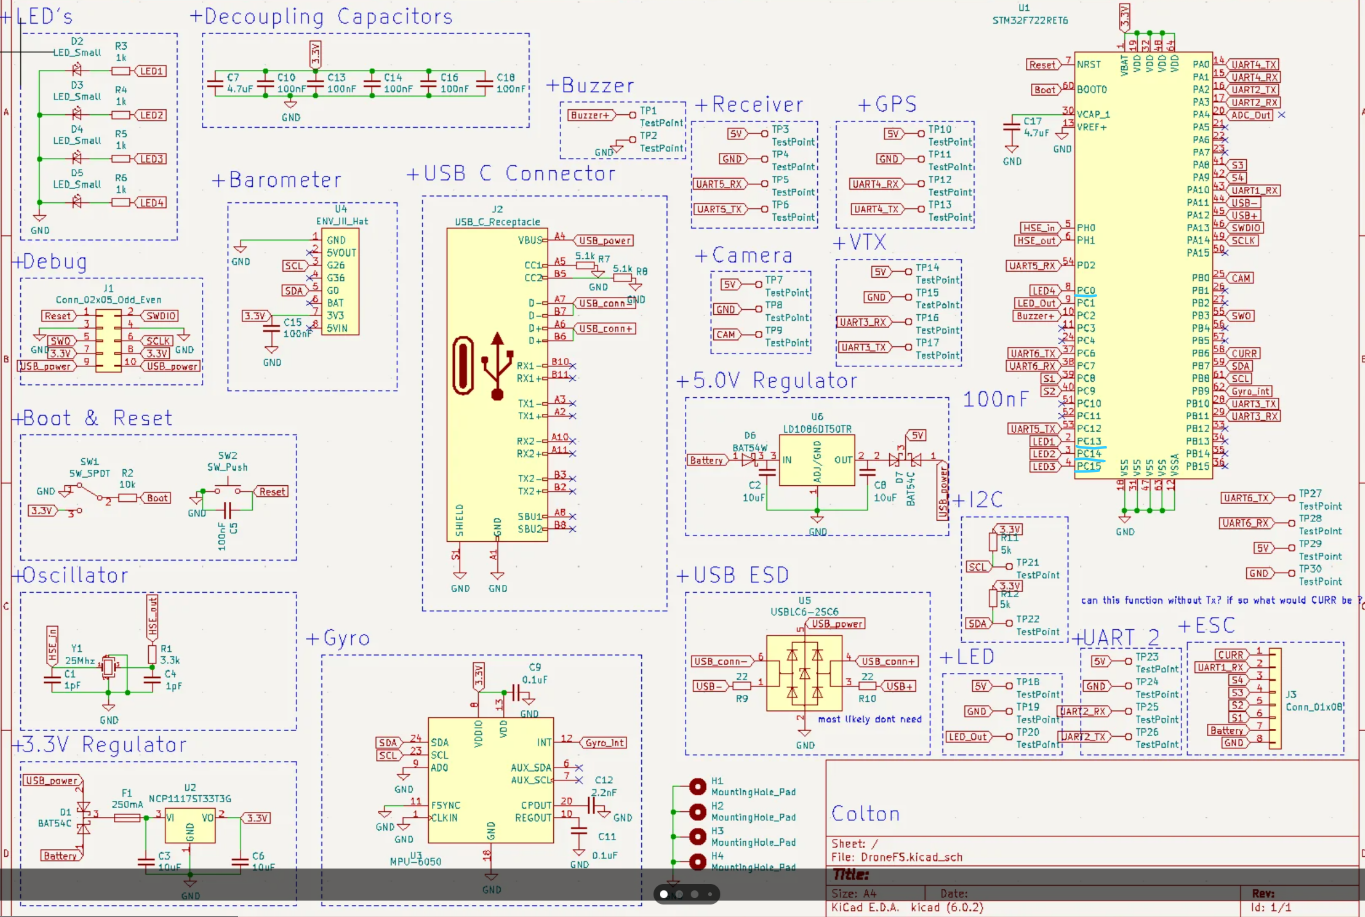
\includegraphics[height=0.3\textheight]{BoardOneNote.png}
	\caption{Schaltplan des Boards in OneNote.}
	\label{fig:boardonenote}
\end{figure}

\begin{figure}[h!]
	\centering
	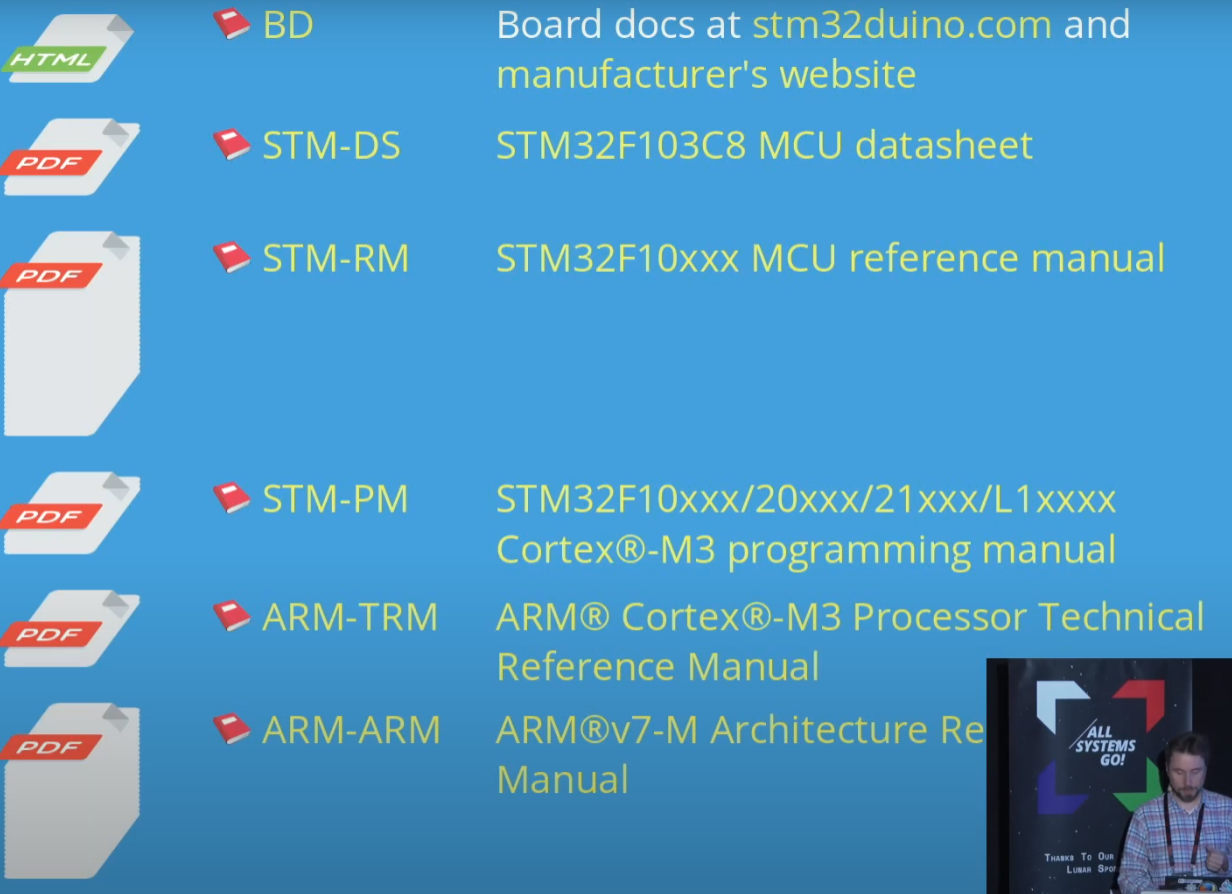
\includegraphics[height=0.3\textheight]{Docs.png}
	\caption{Screenshot von Dokumenten.}
	\label{fig:docs}
\end{figure}

\begin{figure}[h!]
	\centering
	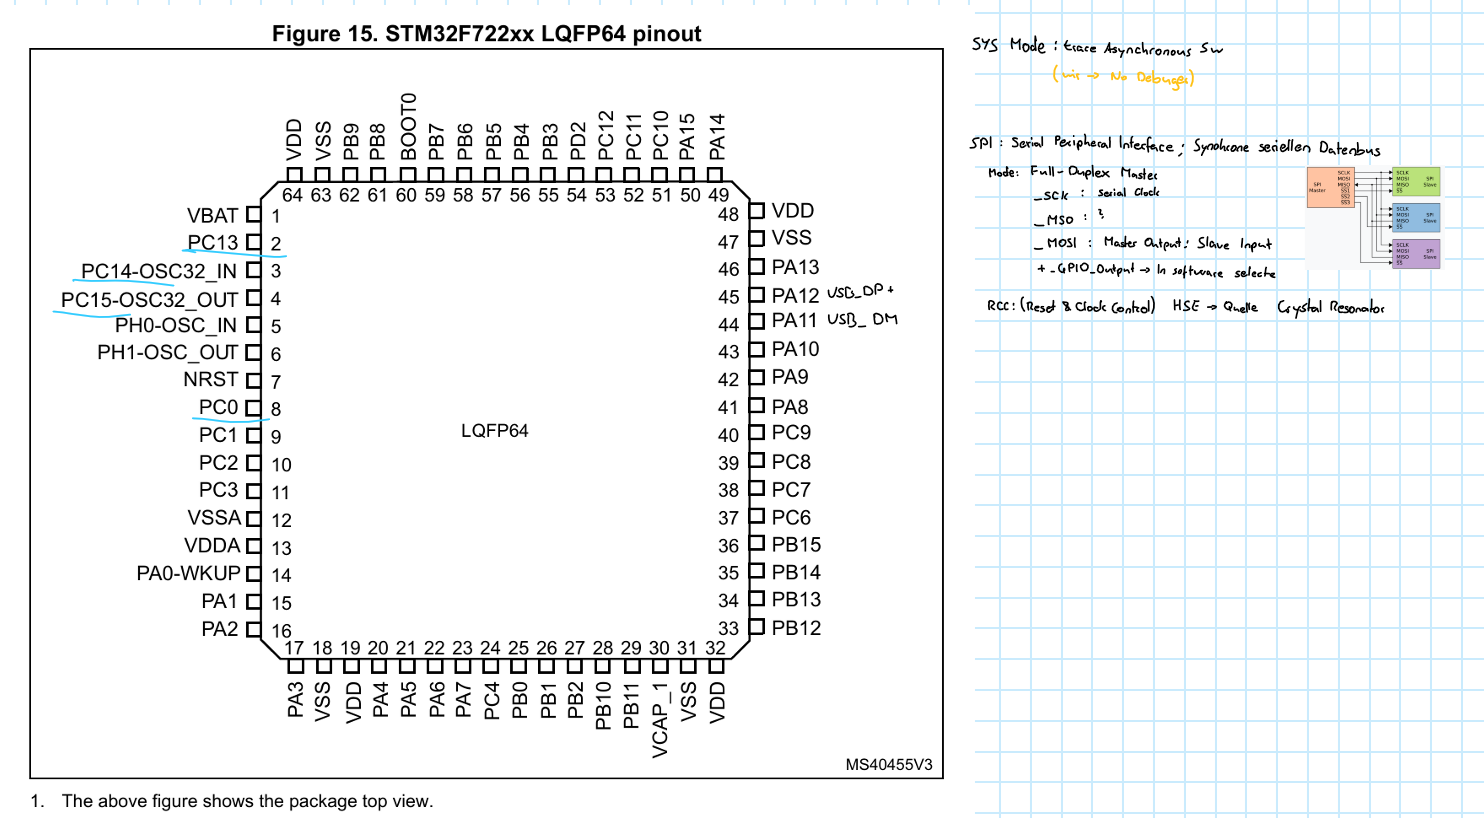
\includegraphics[height=0.3\textheight]{Figure15.png}
	\caption{Eine technische Abbildung (Figure 15).}
	\label{fig:figure15}
\end{figure}

\begin{figure}[h!]
	\centering
	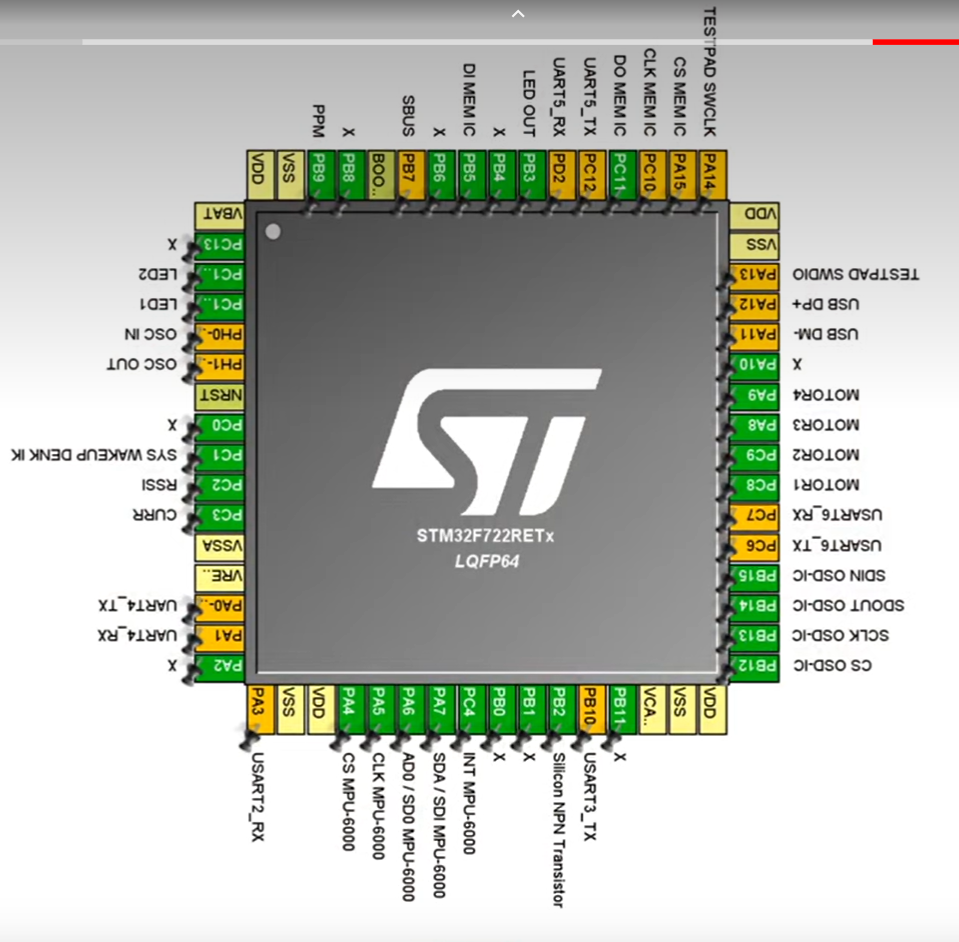
\includegraphics[height=0.3\textheight]{MambaF7.png}
	\caption{Mamba F7 Flight Controller.}
	\label{fig:mambaf7}
\end{figure}

\begin{figure}[h!]
	\centering
	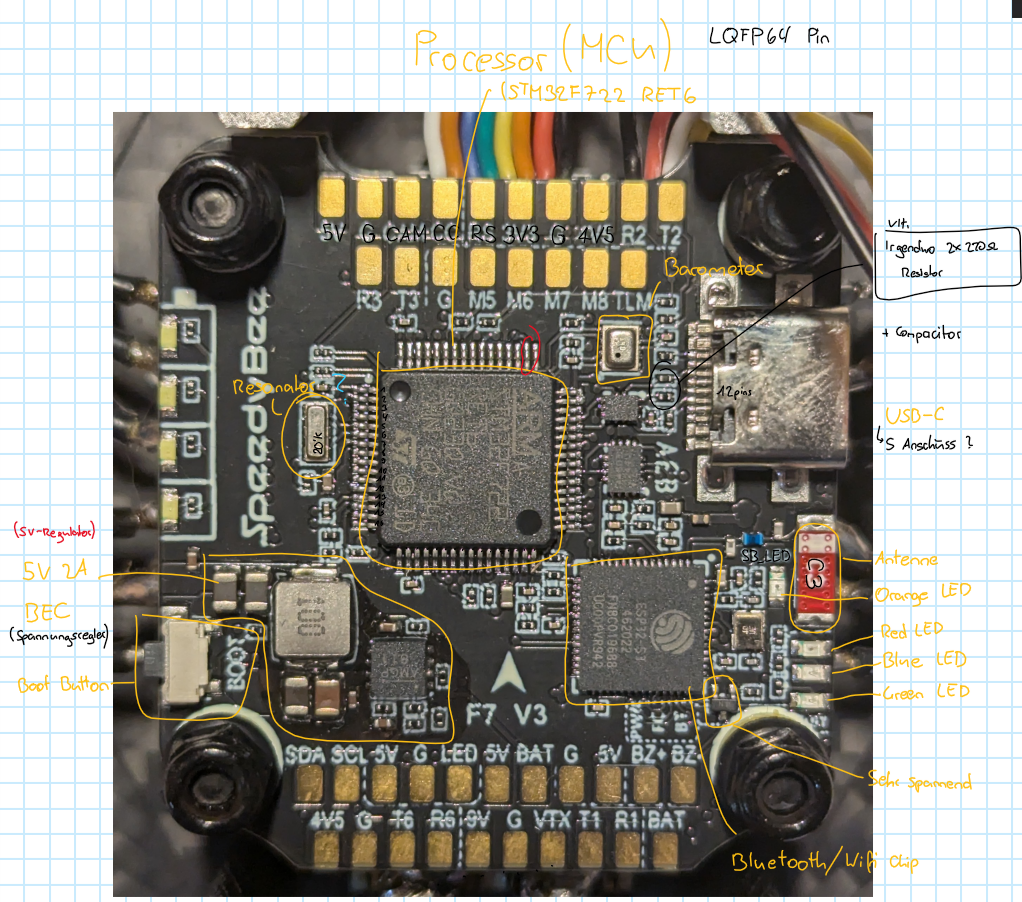
\includegraphics[height=0.3\textheight]{OneNote1.png}
	\caption{Schaltplan aus OneNote - Teil 1.}
	\label{fig:onenote1}
\end{figure}

\begin{figure}[h!]
	\centering
	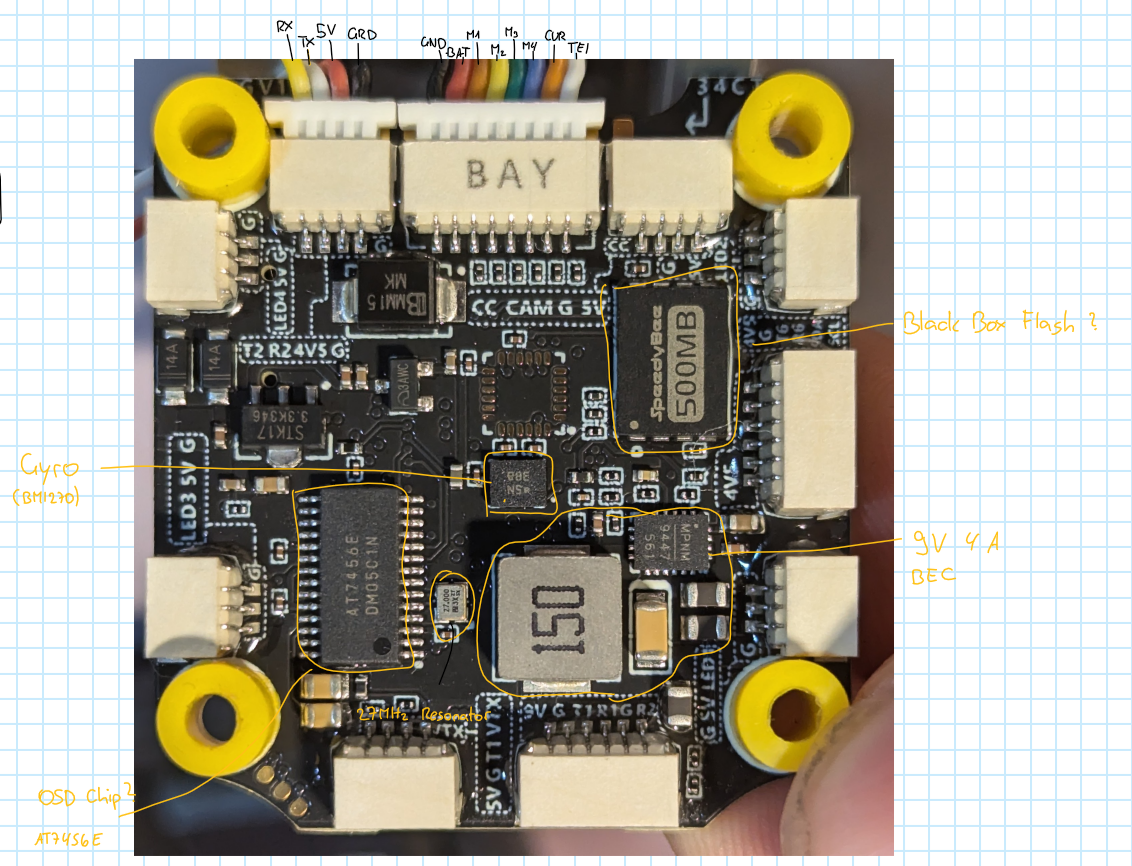
\includegraphics[height=0.3\textheight]{OneNote2.png}
	\caption{Schaltplan aus OneNote - Teil 2.}
	\label{fig:onenote2}
\end{figure}

\begin{figure}[h!]
	\centering
	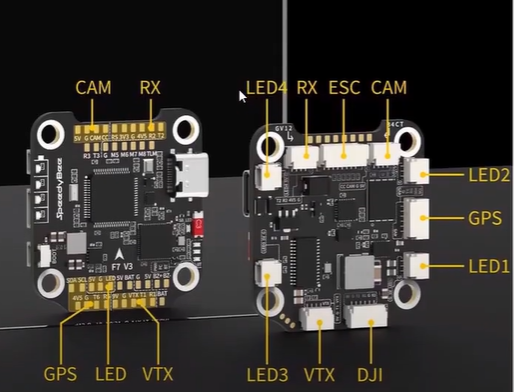
\includegraphics[height=0.3\textheight]{OneNote3.png}
	\caption{Schaltplan aus OneNote - Teil 3.}
	\label{fig:onenote3}
\end{figure}

\begin{figure}[h!]
	\centering
	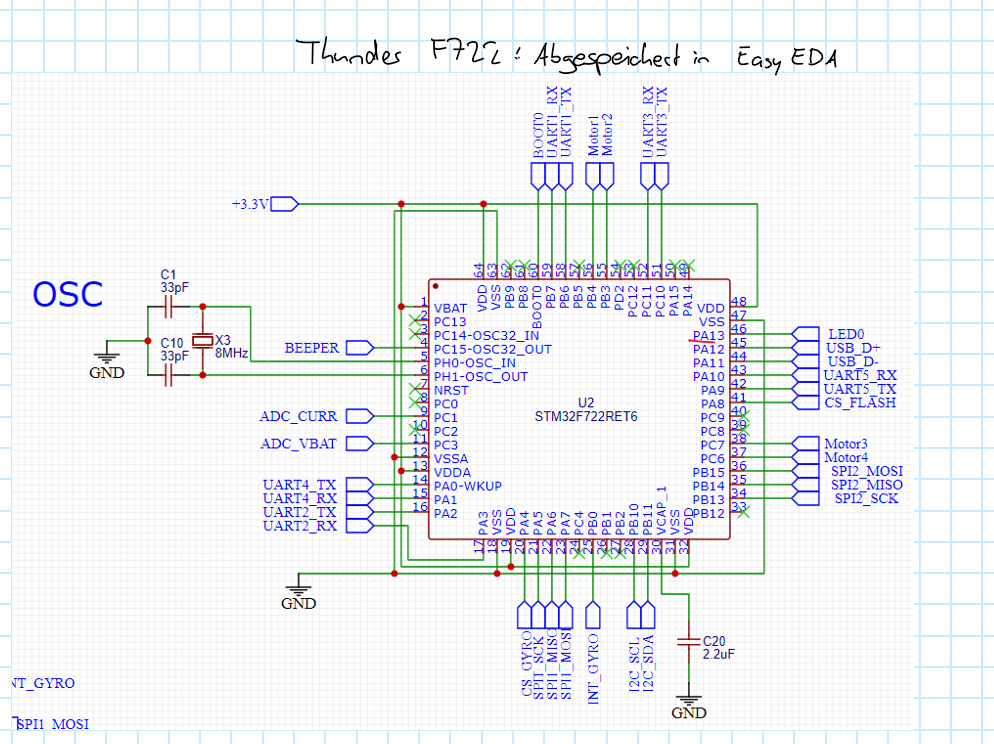
\includegraphics[height=0.3\textheight]{ThunderF722.png}
	\caption{Thunder F722 Schaltplan.}
	\label{fig:thunderf722}
\end{figure}

\begin{figure}[h!]
	\centering
	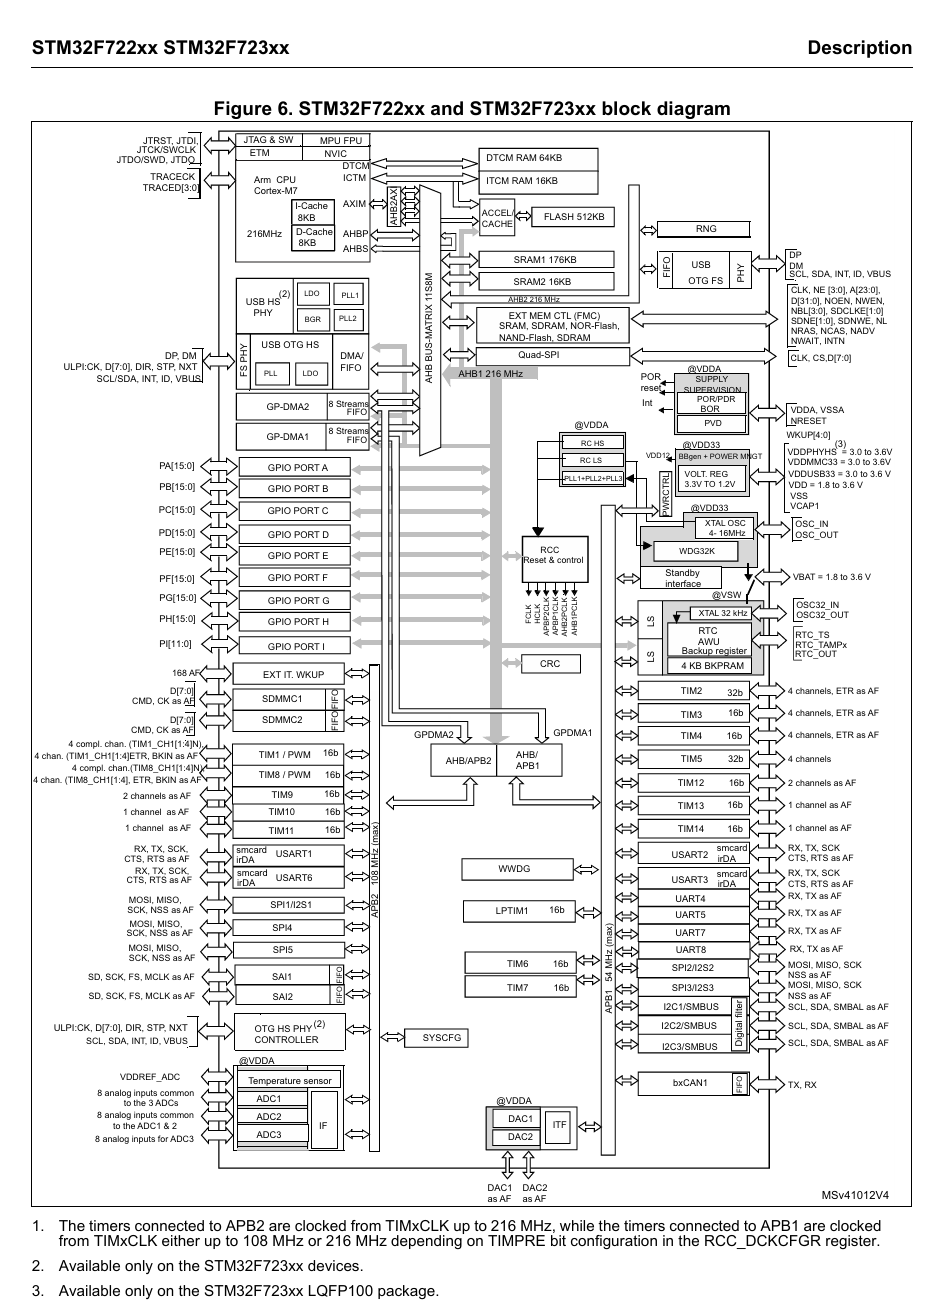
\includegraphics[height=0.5\textheight]{STM32F722xx.png}
	\caption{STM32F722xx Übersicht.}
	\label{fig:stm32f722xx}
\end{figure}

% ab hier ist es nicht von uns sonder von der Vorlage

%\input{unnötig}
%\chapter{Literatur und Bib\TeX} \label{ch:literatur}
\section{Literatur-Verweise}
Literaturangaben in \LaTeX{} \cite{lamport-latex} werden in einem
separaten <<.bib>>-File gespeichert und dann im Code mit <<{\tt$\backslash$cite\{{\em name}\}}>> eingebunden. 
Es werden am Schluss automatisch nur jene aufgeführt, die auch tatsächlich im
Text referenziert wurden. Überschüssige Literaturangaben in der .bib-Datei 
stören nicht und sollten auch nicht gelöscht werden, die könnten später noch
einmal nützlich sein.

Zusätzliche können beim Verweis noch die Seitenzahlen angegeben werden, wie 
im folgenden Beispiel:
\begin{quote}
Es folgt eine mathematisch strenge Herleitung, die im Jahre 1953 in einer russischen Mathematikzeitschrift
	veröffentlicht wurde~\cite[181-182]{formula-derivation}.
\end{quote}
Die Referenz wird mit 
\begin{verbatim}
\cite[181-182]{formula-derivation}
\end{verbatim}
eingebunden. Der Eintrag in der .bib-Datei (in diesem Fall die Datei
literatur.bib) sieht wie folgt aus:

\begin{verbatim}
@book{formula-derivation,
    author={A. M Yaglom and I. M. Yaglom},
    title= {An elementary derivation of the formulas of Wallis, 
	                      Leibniz and Euler for the number pi.},
    publisher = {Uspekhi Mat. Nauk},
    volume={Volume 8},
    year={1953}
}
\end{verbatim}

\subsection{Die .bib-Datei}
Es lohnt sich, zuerst online nach einem fertigen Eintrag zu
suchen. Das ist oft schneller und bequemer, als selbst einen zu
erstellen. Es gibt auch Programme, die
leere Einträge erstellen. Oder man kopiert einen ähnlichen
Eintrag und ändert diesen ab.
Mehr zum Format der Einträge online \cite{bibtex}.


\subsection{ISBN to Bib\TeX{}Converter}
Mit online <<ISBN to Bib\TeX{} Converter>>
\cite{isbn2bibtex} können auch ISBN-Nummern direkt in
Bib\TeX{}-Einträge übersetzt werden (der Amazon-Link darf dabei
hemmungslos gelöscht werden).

\subsection{Kompilierung}
Diese Vorlage verwendet <<biber>>\cite{bibtex-with-biber}. Das Programm muss
eventuell noch separat installiert werden.

\newpage
\section{Interne Verweise} \label{sec:verweise-intern}
Nach jedem Befehl, der eine Nummer erzeugt, 
kann ein <<label>> platziert werden, den 
dann mit <<autoref>> referenziert werden kann, 
siehe \autoref{fig:verweise-intern}.


\begin{figure}[ht]
\centering
\begin{minipage}{0.8\textwidth}
\begin{verbatim}
\section{Interne Verweise} \label{sec:verweise-intern}
Nach jedem Befehl, der eine Nummer erzeugt, 
kann ein <<label>> platziert werden, den 
dann mit <<autoref>> referenziert werden kann, 
siehe \autoref{fig:verweise-intern}.

\begin{figure}[ht]
\centering
\begin{minipage}{0.8\textwidth}

	...

\end{minipage}
	\caption{Code-Beispiel zu \autoref{sec:verweise-intern}}
	\label{fig:verweise-intern}
\end{figure}
\end{verbatim}
\end{minipage}
	\caption{Code-Beispiel zu \autoref{sec:verweise-intern}}
	\label{fig:verweise-intern}
\end{figure}



 %       \
%\chapter{Grafiken\index{Grafiken}}\label{sec:grafiken}
\section{Wichtigste Punkte}
\begin{itemize}
	\item Schematische Darstellungen sollten wenn irgendmöglich vektoriell sein.
		Anstatt Screen\-shots wenn möglich als pdf <<drucken>> und dann das pdf
		vektoriell bearbeiten (z.B. mit Inkscape oder LibreOffice).
	\item In Graphen sind alle Achsen beschriftet, inkl. Masseinheiten.
	\item Sämtliche Zahlen müssen erklärt sein, entweder direkt in der Grafik
		oder in der Legende dazu.
	\item Jede Grafik wird mit einer Legende (<<$\backslash$caption>>) und einem
	<<$\backslash$label>> versehen. Dadurch erhält jede Grafik eine Nummer und wird
	automatisch im Abbildungsverzeichnis (<<$\backslash$listoffigures>>) aufgeführt.
%
	\item Jede Grafik muss im Text erwähnt werden (<<$\backslash$autoref>>).
\end{itemize}

\begin{wrapfigure}{r}{0.6\textwidth}
	\centering
	\includegraphics[width=0.55\textwidth]{wrapfig-code.pdf}
	\captionof{figure}{Code für die \autoref{fig:wrapfig}.}
	\label{fig:wrapfig}
\end{wrapfigure}


\LaTeX{} platziert die Grafik nicht unbedingt dort, wo man es
erwartet. Abhilfe kann da z.B. <<wrapfigure>> bieten.

Dieser Paragraph ist ein Beispiel dazu, der nötige 
\LaTeX-Code ist in der \autoref{fig:wrapfig} zu finden.


\section{Vektorgrafiken}
Ideal sind Vektorgrafiken (.pdf oder .svg Formate). Diese können über
Umwege auch unter Windows produziert werden:
\begin{itemize}
\item Erstellen Sie Ihre Grafik mit einem Programm (aber nicht ein
  Pixelbasiertes Programm wie z.B. Paint, Gimp oder Photoshop),
  sondern z.B. Excel oder Powerpoint. Konvertieren Sie dann die Grafik
  ins pdf-Format, indem Sie einen <<pdf-Drucker>> installieren und die
  Grafik darauf <<ausdrucken>>.
\item Sie können aber auch OpenOffice Calc/Draw oder Inkscape
  verwenden. Diese frei verfügbaren Programme können direkt im
  .pdf-Format oder .svg-Format speichern.
\item Bearbeiten Sie dann die Grafiken, falls nötig, mit Inkscape
  (frei verfügbar).
\end{itemize}

\subsection{Vektorielle Screenshots von Webseiten}
Als pdf Drucken, danach in Inkscape bearbeiten.

Wenn man möchte, dass die Seite aussieht wie auf dem Bildschirm,
kann in Chrome wie folgt vorgegangen werden:
\begin{itemize}
	\item Entwicklertools öffnen (F12).
	\item Im Hamburgermenu <<More Tools>> $\leftarrow$ <<Rendering>>
	\item Emulate Rendering type: <<screen>>.
	\item Dann <<ausdrucken als pdf>>.
	\item pdf nötigenfalls bearbeiten.
\end{itemize}

\section{Einbinden einer Grafik}

\begin{figure}[ht] % try placing 'h'ere, then 't'op of next page
    \centering
    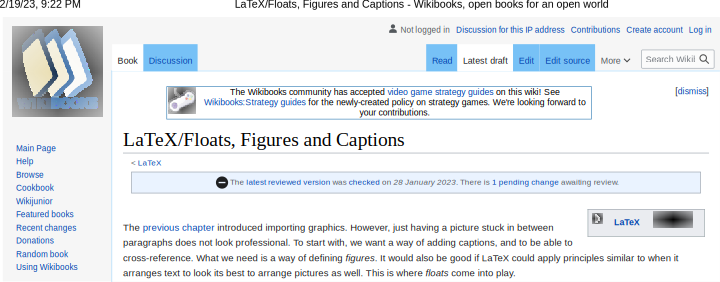
\includegraphics[width=0.8\textwidth]{wikibooks-figures.pdf}
    \caption[Wikibooks]{Screenshot der Wikibooks website \cite{figures}. Beachten
        Sie, dass der Text in dieser Grafik sogar selektierbar ist.}
    \label{fig:wikibooks}
\end{figure}

Dazu muss gar nicht viel gesagt, weil schon alles
auf Wikibooks \cite{figures} gefunden werden kann, 
wovon in \autoref{fig:wikibooks} ein
Screenshot zu sehen ist. Der \LaTeX-Code ist in 
\autoref{lst:figure-example} zu finden.

\subsection{\LaTeX-Code}
Zum Einbinden der \autoref{fig:wikibooks}
wurde der \LaTeX-Code im Listing 
\ref{lst:figure-example} verwendet.

\lstinputlisting[
label=lst:figure-example,
language=tex,
caption={Code zum Einbinden der \autoref{fig:wikibooks}.},
]{graphics-figure-example.tex}
 %        \
%\chapter{Kompilierung}\label{sec:compilieren}

\section{Technischer Ablauf}
\LaTeX-Dateien (Dateiendung \texttt{.tex})
sind einfache Text-Dateien (d.h. nur Buchstaben, keine
Formatierung). 
Sie können mit einem beliebigen Text-Editor bearbeitet werden.
Spezialiserte Editoren oder Modi sind aber empfehlenswert.\\
%
Aus den \LaTeX-Dateien wird dann eine PDF-Datei erzeugt.
Diesen Vorgang nennt man {\em kompilieren}.\\
%
Bei der Kompilierung gibt es mehrere Schritte, die bis auf einen
vom Programm \texttt{pdflatex} erledigt werden.
\begin{itemize}
	\item Setzen des Text und <<Sammeln>> der Verweise.
	\item Abermaliges Setzen und Einfügen der Verweise.
	\item Setzen des Literaturverzeichnisses 
		(hier mit \texttt{biber}, früher mit \texttt{bibtex}).
	\item Abermaliges Setzen und Einfügen der Verweise.
\end{itemize}
Je nach Editor müssen diese Schritte manuell angestossen werden
oder erfolgen automatisch (z.B. mit \TeX{}Studio) oder dem 
beiliegenden \texttt{Makefile}, siehe \autoref{sec:make}.

\section{Installation der Software}

\subsection{Windows}\label{sec:windows}
Für alle \LaTeX{}-Pakete und Programme zur Kompilierung wird
MiK\TeX{} empfohlen, hier zu finden:
\begin{center}
\url{https://miktex.org/download}
\end{center}
\noindent Bei der Installation empfehle ich alle default-Einstellung, bis
auf die Einstellung 
<<{\em Pakete ohne Nachfrage automatisch nachinstallieren}>>, die
ich empfehlen kann.

Nach der Installation soll gerne nach Updates gesucht werden. Diese werden nach
ca. 1 min auch zur Installation angeboten und sollten dann eingespielt werden.


\noindent Als Editor kann ich \TeX{}studio empfehlen, hier zu finden:

\begin{center}
\url{https://www.texstudio.org/}
\end{center}

\noindent Von \TeX{}live und \TeX{}works kann ich nicht viel Gutes berichten.


\subsection{Mac}
Da gibt es offenbar \href{https://tug.org/mactex/}{MacTeX
  (https://tug.org/mactex/)}. Wird wohl gut sein.

\subsection{Cloud-Lösung Overleaf}
Cloud-Lösung für \LaTeX. Sorgen Sie für ein regelmässiges lokales
Backup (wie bei allen Cloud-Diensten sind Ihre Daten auf fremden Datenträgern).

\subsection{Linux}\label{sec:linux}
Für Ubuntu sollten folgende Pakete installiert werden:\\[2mm]
%
\texttt{
sudo apt install texlive-latex-base texlive-pictures texlive-science\\ 
sudo apt install texlive-latex-extra texlive-lang-german biber
}\\[2mm]
Hinweis: \TeX{}studio gibt es auch für Linux.

\section{Kompilierung mit make}\label{sec:make}
Das Programm \texttt{make} erlaubt es, Abhängigkeiten zu definieren
wie aus welchen Dateien weitere erzeugt werden sollen. Das wird normalerweise
in der Softwareentwicklung verwendet, eignet sich aber auch für die 
Kompilierung dieses Dokuments.\\
%
Das Programm \texttt{make} kann durch Installation des 
folgendes Pakets installiert werden:

\texttt{
	sudo apt install build-essential
}

\noindent Für diese Vorlage wurde das Makefile in \autoref{lst:makefile} verwendet.

\lstinputlisting[
	language=make,
	label=lst:makefile,
	caption={[Makefile]Das Makefile, das diese Dokument kompiliert.},
% linerange={88-93},firstnumber=88
]{Makefile}


Die einzelnen Kommandos können natürlich auch manuell eingegeben
werden. Gerade für grössere Projekte eignen sich Makefiles aber, da
alle Abhängigkeiten spezifiziert werden können. Z.B.\ können auch
programmatisch erzeugte Grafiken automatisch neu erstellt werden, wenn
die zugrundeliegenden Daten sich ändern.

 %     \
%\chapter{Mathematik in \LaTeX}\label{sec:mathezeugs}
Es empfiehlt sich die <<amsmath>> package einzubinden, mit
\begin{verbatim}
\usepackage{amsmath}
\end{verbatim}

\section{Gleichungen}
Je nach Layout gibt es verschiedene Umgebungen. Gute Beispiele finden sich auch
in \LaTeX{}-Dokumentation von Overleaf\cite{overleaf-equations}.
\subsection{Einzeiler}
Normalerweise kriegen alle Gleichungen eine Nummer wie die
\autoref{eq:erstes-beispiel} und werden im Text referenziert.
\begin{equation} \label{eq:erstes-beispiel}
	B > \frac{1}{n} \sum_{i=1}^n x_i
\end{equation}
%
Die \autoref{eq:erstes-beispiel} wurde durch den Code in
\autoref{lst:erstes-beispiel} erzeugt:
%\begin{latexcode}[Code zu \autoref{eq:erstes-beispiel}]%[erstes-beispiel]
\begin{latexcode}[{Code zur \autoref{eq:erstes-beispiel}}]{lst:erstes-beispiel}
\begin{equation} \label{eq:erstes-beispiel}
    B > \frac{1}{n} \sum_{i=1}^n x_i
\end{equation}
\end{latexcode}


\noindent Soll eine Gleichung oder Formel ausnahmsweise keine Nummer erhalten wie in
\[
	E = mc^2,
\]
kann der Code in \autoref{lst:keine-nummer} verwendet werden.
\begin{latexcode}[{Nicht nummerierte Gleichung}]{lst:keine-nummer}
\[
    E = mc^2
\]
\end{latexcode}

\subsection{Mehrzeiler}
Um Umformungen von Gleichungen darzustellen, 
eigenet sich die {\tt aligned} Umgebung, wie in 
\autoref{eq:gleichungumformen} zu sehen:
\begin{equation} \label{eq:gleichungumformen}
	\begin{aligned}
		-\frac{6}{7}x = & -\frac{10}{3}+\frac{4}{7}x & & | -\frac{4}{7}x\\
		-\frac{10}{7}x  = & -\frac{10}{3} & & | : -\frac{10}{7}\\
		x  = & \frac{7}{3} \\
	\end{aligned}
\end{equation}
Der Code dazu gibt es in \autoref{lst:gleichungumformen}.
Ganz ähnlich wie {\tt aligned} funktioniert die {\tt align}-Umgebung 
(alleine, nicht innerhalb einer {\tt equation} Umgebung), 
die dann aber jede
Zeile durchnummeriert, was durchaus auch nützlich sein kann.
\begin{latexcode}[Code zur \autoref{eq:gleichungumformen}]{lst:gleichungumformen}
\begin{equation} \label{eq:gleichungumformen}
    \begin{aligned}
        -\frac{6}{7}x = & -\frac{10}{3}+\frac{4}{7}x & & | -\frac{4}{7}x\\
        -\frac{10}{7}x  = & -\frac{10}{3} & & | : -\frac{10}{7}\\
        x  = & \frac{7}{3} \\
    \end{aligned}
\end{equation}
\end{latexcode}


%
Sollen einfach längere Umformungen dargestellt werden
eignet sich die {\tt multline} Umgebung:
\begin{multline} \label{eq:langeumformung}
	f'(x) = \lim_{h \to 0} \frac{f(x+h)-f(x)}{h} = 
	\lim_{h \to 0} \frac{a^{x+h}-a^x}{h} =  \\
	\lim_{h \to 0} \frac{a^x \cdot a^h-a^x}{h} = 
	\lim_{h \to 0} \frac{a^x \cdot \left(a^h-1\right)}{h} =  \\
	a^x \cdot \lim_{h \to 0} \frac{a^{0+h}-a^0}{h} = a^x \cdot f'(0)	
\end{multline}

Der Code zu \autoref{eq:langeumformung} ist in \autoref{lst:langeumformung}
dargestellt.
\begin{latexcode}[Code zur \autoref{eq:langeumformung}]{lst:langeumformung}
\begin{multline} \label{eq:langeumformung}
    f'(x) = \lim_{h \to 0} \frac{f(x+h)-f(x)}{h} = 
    \lim_{h \to 0} \frac{a^{x+h}-a^x}{h} =  \\
    \lim_{h \to 0} \frac{a^x \cdot a^h-a^x}{h} = 
    \lim_{h \to 0} \frac{a^x \cdot \left(a^h-1\right)}{h} =  \\
    a^x \cdot \lim_{h \to 0} \frac{a^{0+h}-a^0}{h} = a^x \cdot f'(0)
\end{multline}
\end{latexcode}

\section{Vektoren}

\begin{equation}\label{eq:erste}
\vec v = \begin{pmatrix}
a_1\\
a_2\\
a_3
\end{pmatrix}
\end{equation}

Verwendet man \autoref{eq:erste} dann erhält man:

\begin{equation}\label{eq:zweite}
\vec u = \begin{pmatrix}
a_1+b_1\\
a_2-\pi\\
a_3+\cos\left(\alpha^2\right)
\end{pmatrix}
\end{equation}

Der Code dazu ist in \autoref{lst:latex-code} ersichtlich.

\begin{latexcode}[Code zu \autoref{eq:erste} und \autoref{eq:zweite}]{lst:latex-code}
\begin{equation}\label{eq:erste}
\vec v = \begin{pmatrix}
a_1\\
a_2\\
a_3
\end{pmatrix}
\end{equation}

Verwendet man \autoref{eq:erste} dann erhält man:

\begin{equation}\label{eq:zweite}
\vec u = \begin{pmatrix}
a_1+b_1\\
a_2-\pi\\
a_3+\cos\left(\alpha^2\right)
\end{pmatrix}
\end{equation}

Den Code dazu ist in \autoref{fig:latex-code} ersichtlich.
\end{latexcode} %      \
%\chapter{Darstellung}
Die Titel vom Kapitel und Unterkapitel werden
in der Kopfzeile angezeigt. Wenn die zu lange sind, können alternative, kürzere Titel für die Kopfzeile und das Inhaltsverzeichnis verwendet werden.
\section[Gekürzter Titel]{Verdammt langer Titel, der nicht in die Kopfzeile passt}

Anfrage an ChatGPT:
	\begin{quote}
When writing a report with documentclass$\{$report$\}$, how can I prevent long section titles from overflowing the page header?
	\end{quote}
\noindent
Und die Antwort:
	\begin{quote}
To prevent long section titles from overflowing the page header in a LaTeX
		document using the report document class, you can use the short optional
		argument for the $\backslash$section command to specify a shorter version of the section title to be used in the page header. Here's an example (\autoref{lst:shorttitleoption}):

\begin{latexcode}[Optionaler kurzer Titel]{lst:shorttitleoption} % Das ist in vorlage.txt in Zeile 133 definiert
\documentclass{report}
\begin{document}
\section[Short Title]{Long Section Title That May Overflow the Header}
Text of the section goes here.
\end{document}
\end{latexcode}
In this example, the short version of the section title is specified within square brackets []. This short title will be used in the page header instead of the full title.

\newpage
Alternatively, you can manually set the header using the $\backslash$markboth command. Here's an example (\autoref{lst:markboth}):
\begin{latexcode}[Beide Titel (links und rechts) überschreiben]{lst:markboth}
\section{Long Section Title That May Overflow the Header}
\markboth{Short Title}{Short Title}
\end{latexcode}

In this example, $\backslash$markboth sets both the left and right page headers to "Short Title", effectively overriding the automatic section title inclusion. You can adjust the short title to your liking.

	\end{quote}
%\chapter{Massangaben}\label{sec:massangaben}

Sobald Masseinheiten angegeben werden, lohnt sich das package
{\tt siunitx}\cite{siunitx}.


\section{Beispiele}
Mehr Beispiele finden Sie in der offiziellen Dokumentation des package.
\begin{itemize}
	\item Beschleunigung $g = \qty{9.81}{\metre\per\square\second}$. 
	\verb+$g = \qty{9.81}{\metre\per\square\second}$+
%
	\item Strom $I = \qty{25}{\micro\ampere}$.
		\verb+$I = \qty{25}{\micro\ampere}$+
	\item Widerstand $R = \qty{2}{\mega \ohm}$.
		\verb+$R = \qty{2}{\mega \ohm}$+
\end{itemize}

\section{Alte Version (v2) von siunitx}
Sollte Ihr System noch eine alte Version von siunitx haben, verwenden Sie
anstatt \verb+\qty+ den Befehl \verb+\SI+, also z.B.

\verb+\SI{25}{\micro\ampere}  +
anstatt
\verb+   \qty{25}{\micro\ampere}+

Siehe auch \cite{qty-vs-si}.
 %      \
%\chapter{Chemie}\label{sec:chemie}
Mit dem alleinigen zusammenbau einer Drohne ist eine Fliegende drohne noch längst nicht geschaft. Als nächstes muss man die Kommunikation zwischen Fernbedienung und Drohne sicherstellen.  



\section{Der Sender (Fernbedienung)}
Es gibt mehrere Packages. Exemplarisch ist hier das <<mhchem>>\cite{mhchem}
Package vorgestellt:


\section{Der Empfänger} \label{sec:chemie-verwendung}
Am besten lesen Sie die Dokumention des Packages, das ist voll mit vielen
Beispielen. Hier sind einige daraus:

\ce{H2O}

\ce{Na+} und \ce{Cl-}

\ce{^{227}_{90}Th}

Der entsprechende Code ist in \autoref{fig:chemie} zu finden.

\begin{figure}[ht]
\centering
\begin{minipage}{0.8\textwidth}
\begin{verbatim}
\ce{H2O}

\ce{Na+} und \ce{Cl-}

\ce{^{227}_{90}Th}
\end{verbatim}
\end{minipage}
\caption{\LaTeX{}-Code, der die chemischen Formeln in
	\autoref{sec:chemie-verwendung}
erzeugt.}
\label{fig:chemie}
\end{figure}
 %      \
%\chapter{Einbinden von Code}\label{sec:code}
Vollständige Code-Listings gehören nicht in den Bericht, sondern 
die dem Bericht beigelegte SD-Karte.\footnote{Wobei das nicht mehr erlaubt ist,
wie die Codes der Arbeit archiviert werden sollen, erschliesst sich
mir nicht.}

Schlüsselstellen in einem Programm machen aber durchaus Sinn,
aufgeführt zu werden. Ein Beispiel für Python-Code 
finden Sie im \autoref{lst:python-code}.

Für \LaTeX-Code finden Sie ein Beispiel im \autoref{lst:figure-example}.

Im \autoref{lst:javaquine} auf der nächste Seite ist das
Listing eines Quines abgebildet (ein Programm, das seinen eigenen Source-Code als
Ausgabe produziert).

\section{Python Code}
\lstinputlisting[
label=lst:python-code,
language=python,
caption={Python-Code zur Erzeugung des Pascaldreiekcs},
]{code/pascal.py}

\newpage
\section{Java Code}
\lstinputlisting[
label=lst:javaquine,
caption={[JavaQuine]Ein Java Quine\cite{javaquine}},
% linerange={88-93},firstnumber=88
]{\codefile{Quine}}
 %            \
%\documentclass{beamer}

\usepackage[german]{babel}        % Deutschsprachige Beschriftungen
\usepackage[utf8]{inputenc}       % Utf8 Zeichensatz
\usepackage{graphicx}             % Grafiken
\usepackage{fancyvrb}             % Für VerbatimInput




% See https://www.overleaf.com/learn/latex/Beamer#:~:text=package%20in%20Overleaf-,Reference%20guide,-Below%20is%20a
\usetheme{Warsaw}
\usecolortheme{default}

\beamertemplatenavigationsymbolsempty
\setbeamertemplate{footline}[frame number]

%Information to be included in the title page:
\title{\LaTeX{} für die Maturaarbeit}
\author{Ivo Blöchliger}
\institute{Kantonsschule am Burggraben}
\date{29. August 2023}
\logo{\includegraphics[width=1.5cm]{images/ksbg-logo-no-text.pdf}}

\begin{document}

\frame{\titlepage}

\begin{frame}
\frametitle{Übersicht}
\tableofcontents
\end{frame}

\begin{frame}
	\frametitle{Download der Software}
	\begin{block}{\LaTeX{} Distribution}
		Downalod von Mik\TeX
	\end{block}
	\begin{block}{Editor}
		Download von \TeX{}Studio
	\end{block}
	Links auf https://fginfo.ksbg.ch
\end{frame}

\section{Was ist \LaTeX{}?}
\subsection{Geschichte}
\begin{frame}
	\frametitle{\LaTeX{}?}
	\begin{block}{Aussprache}
		Leitägg (oder Leitäch)
	\end{block}
	\begin{block}{Ursprung}
		\TeX{}: Textsatzsystem für Mathematik, 
		1978, Donald Knuth \\ 
		$\quad$ Ziel: Typographisch einwandfreie Dokumente\\[2mm]
		\LaTeX{}: Sammlung von Macros
		1984, Leslie Lamport
	\end{block}
	\begin{alertblock}{
\includegraphics[height=1em]{images/Laser-symbol.pdf}
		Warnung 
\includegraphics[height=1em]{images/Laser-symbol.pdf}}
		Worddokumente können nach längerer Verwendung von \LaTeX{} zu Augenkrebs
		führen.
	\end{alertblock}
\end{frame}



\subsection{Prinzip}
\begin{frame}
	\frametitle{Prinzip von \LaTeX}
	Beschreiben was, nicht wie.
	\begin{block}{Textdatei {\tt prinzip.tex}}
		\VerbatimInput{prinzip.tex}
	\end{block}
\end{frame}


\begin{frame}
	\frametitle{Automatisieren}
	\begin{itemize}
		\item Nummerierungen
		\item Verweise
		\item Verzeichnisse
		\item Formatierungen
	\end{itemize}
\end{frame}

\begin{frame}
	\frametitle{Nummerierungen}
	\begin{block}{$\backslash$label\{bla\} und $\backslash$autoref\{bla\}}
		$\backslash$label\{bla\} {\bf nach} nummererzeugendem Befehl:\\[3mm]
		\begin{quote}
			{\tt $\backslash$section\{Blah
			Blah\}$\backslash$label\{sec:bla\}}\\[3mm]

			{\tt In $\backslash$autoref\{sec:bla\} \ldots}
		\end{quote}
	\end{block}

	\begin{block}{Labelpräfixe}
		\begin{description}
			\item[Kapitel] {\tt ch:bla}\\
			\item[Abschnitte] {\tt sec:bla}\\
			\item[Abbildungen] {\tt fig:bla}\\
			\item[Gleichungen] {\tt eq:bla}\\
		\end{description}
	\end{block}
\end{frame}

\begin{frame}
	\frametitle{Mathematik}
	Mitternachtsformel, Gleichung \ref{eq:quadsol}:
\begin{equation}\label{eq:quadsol}
	x_{1,2} = \frac{-b \pm \sqrt{b^2-4ac}}{2a}
	\qquad b^2-4ac \geq 0,\, a \neq 0
\end{equation}

	\vspace{-6mm}
	\begin{block}{\LaTeX{} Code}
		\VerbatimInput{mathe.tex}
	\end{block}
\end{frame}

\subsection{Kompilierung}
\begin{frame}
	\frametitle{Kompilierung}
	\begin{block}{Erzeugen des Dokuments}
		\begin{enumerate}
			\item Textsatz, Nummerierung, Benötigte Verweise
			\item Evtl.\ Erzeugen des Literaturverzeichnisses
			\item Textsatz, Eintragen aller Verweise, Verzeichnisse
		\end{enumerate}
	\end{block}
	\begin{example}
		Nach dem ersten Durchgang:\\[2mm]
		\begin{quote}
			\rm
			{\large \bf Abschnitt 2.1}\\
			{Wie im Abschnitt ?? ersichtlich, \ldots}
		\end{quote}
	\end{example}
\end{frame}

\begin{frame}
	\frametitle{Automatisches Kompilieren}
	\begin{itemize}
		\item Mehrere Programme nötig
		\item Richtige Reihenfolge
	\end{itemize}
	\begin{block}{Automatisieren}
		\begin{itemize}
			\item TeXStudio (Editor)
			\item Visual Studio Code Plugin (?)
			\item Makefile (make)
		\end{itemize}
	\end{block}
\end{frame}

\subsection{Bilder}
\begin{frame}
	\frametitle{Bilder}

	\begin{block}{Vektoriell bitte!}
		Wenn irgendmöglich vektorielle Bilder verwenden:
		\begin{itemize}
			\item SVG $\leftarrow$ PDF
			\item PDF (wenn nicht einfach Pixelbild)
		\end{itemize}
		Aus Office-Anwendungen: {\bf Print as PDF...}
	\end{block}
	\begin{block}{Wenn Pixel, dann}
		\begin{description}
			\item[PNG] Screenshots, Bilder mit einfarbigen Flächen
			\item[JPG] Photos
		\end{description}
	\end{block}
\end{frame}

\begin{frame}
	\frametitle{Vergleich der Formate}
	\begin{columns}[onlytextwidth]
		\begin{column}{0.33\textwidth}
		  \centering
			PDF (5.5 kB)\\[5mm]
			
\includegraphics[width=\textwidth]{images/vektor.pdf}
		\end{column}
		\begin{column}{0.33\textwidth}
		  \centering
			 PNG (21 kB)\\[5mm]
			
\includegraphics[width=\textwidth]{images/vektor.png}
		\end{column}
		\begin{column}{0.33\textwidth}
		  \centering
			JPG (17 kB)\\[5mm]
			
\includegraphics[width=\textwidth]{images/vektor.jpg}
		\end{column}
	\end{columns}
\end{frame}

\begin{frame}
	\frametitle{Platzierung automatisch, nicht im Textfluss}
	\begin{block}{Gründe}
		\begin{itemize}
			\item Konzipiert für wissenschaftliche Publikation
			\item Abbildungen speziell farbig, eigene Seiten
			\item Layout dem Autor nicht bekannt
			\item Rücksicht auf Textfluss, Seitenfüllung
		\end{itemize}
	\end{block}
	\begin{alertblock}{Nummerieren, referenzieren!}
		\begin{itemize}
			\item Alle Abbildungen sind nummeriert,\\
		 	\item mit Legende versehen\\
			\item und {\bf im Text referenziert}.
		\end{itemize}
	\end{alertblock}
\end{frame}


\section{Software}
\subsection{Absolut nötige Software}
\begin{frame}
	\frametitle{Benötigte Software}
	\begin{itemize}
		\item \LaTeX{} Distribution (z.B. MikTeX oder TeXLive)
			\begin{itemize}
				\item Programme: {\tt pdflatex}, {\tt bibtex}, {\tt biber}, etc.
				\item \LaTeX{} Pakete: {\tt beamer}, {\tt babel}, {\tt graphicx}, etc.
			\end{itemize}
		\item Texteditor: TeXStudio, Visual Studio Code, Vim, \ldots
		\item PDF-Viewer
	\end{itemize}
\end{frame}

\subsection{Nützliche Software}
\begin{frame}
	\frametitle{Nützliche Software}
	\begin{itemize}
		\item Inkscape, LibreOffice (SVG, PDF)
		\item make o.ä. als Buildsystem
		\item Verzeichnisse/Konverter zu Bib\TeX{} Einträgen
		\item Erstellung von \LaTeX{}-Tabellen
	\end{itemize}
\end{frame}



\section{Hilfe!}
\begin{frame}
	\frametitle{Hilfe!}
	\begin{block}{Tech-Lab (E23)}
		Dienstags ab 16:40\\
		Freitags ab 17:20
	\end{block}
	\begin{block}{Teams}
		Fragen und Antworten auf dem \LaTeX{} Team
	\end{block}
	\begin{block}{Vorlage auf Github}
		Ergänzungen, Verbesserungen gerne liefern!
	\end{block}
\end{frame}

\begin{frame}
	\frametitle{Dank}
	\centering
	\Huge
	Herzlichen Dank\\
	für Ihre Aufmerksamkeit\\[1cm]
	Fragen?
\end{frame}

\begin{frame}
	\frametitle{Weiteres Vorgehen}
	\begin{block}{Plan}
		\begin{itemize}
			\item Software installieren
			\item Vorlage herunterladen
			\item Vorlage kompilieren
			\item Minimalbeispiel kompilieren
			\item Minimalbeispiel studieren/ändern
		\end{itemize}
	\end{block}
\end{frame}

\end{document}


% --------------------------

% === Optional: INDEX ====
\cleardoublepage  %      \  
\phantomsection %        \
\addcontentsline{toc}{chapter}{\indexname} 
\printindex %            \
% ------------------------


% === ABBILDUNGSVERZEICHNIS ===
\cleardoublepage %             \
\phantomsection %              \
\addcontentsline{toc}{chapter}{\listfigurename}
\listoffigures %               \
% -----------------------------

% === CODEBLOCKVERZEICHNIS ===
\cleardoublepage %            \
\phantomsection %             \
\addcontentsline{toc}{chapter}{\lstlistlistingname}
\lstlistoflistings %          \
% ----------------------------

% === LITERATURVERZEICHNIS ===
\cleardoublepage %            \
\phantomsection %             \
\addcontentsline{toc}{chapter}{\bibname}
\printbibliography %          \
% ----------------------------
% =========== START VON ANHÄNGE ===========
\appendix

% === EIGENSTÄNDIGKEITSERKLÄRUNG ===
\chapter{Eigenständigkeitserklärung}\label{ch:appendix_independencedeclaration}

Wir bestätige mit unseren Unterschriften, dass wir unsere Maturaarbeit selbständig verfasst und in schriftliche Form gebracht haben, dass sich die Mitwirkung anderer Personen auf Beratung und Korrekturlesen beschränkt hat und dass alle verwendeten Unterlagen und Gewährspersonen aufgeführt sind. Uns ist bekannt, dass eine Maturaarbeit, die nachweislich ein Plagiat gemäss der in der Maturaarbeitsbroschüre gegebenen Definition darstellt, als schwerer Verstoss im Sinne des Maturitätsprüfungsreglements gewertet wird.

\vspace{3cm}

\noindent
\begin{tabular}{p{0.47\linewidth}p{0.47\linewidth}}
  Ort \&\ Datum & Unterschrift \\
  & \\[1cm]
  \hline
\end{tabular}
\vspace{3cm}

\noindent
\begin{tabular}{p{0.47\linewidth}p{0.47\linewidth}}
	Ort \&\ Datum & Unterschrift \\
	& \\[1cm]
	\hline
\end{tabular}

% ----------------------------------


\chapter{Informationen über die Teile}\label{ch:infoteile}
\renewcommand{\arraystretch}{1.3} % Optional: Erhöht den Zeilenabstand in der Tabelle

\begin{longtable}{|l|p{4cm}|p{4cm}|p{4cm}|}
	\caption{Übersicht der technischen Komponenten der Drohne} \label{tab:DrohnenKomponenten} \\ \hline
	\textbf{Komponente}       & \textbf{Details}                                                                                                   & \textbf{Funktion}                                                                                                           & \textbf{Besondere Merkmale}                                                                                     \\ \hline
	\endfirsthead % Kopfzeile für die erste Seite
	
	\hline
	\textbf{Komponente}       & \textbf{Details}                                                                                                   & \textbf{Funktion}                                                                                                           & \textbf{Besondere Merkmale}                                                                                     \\ \hline
	\endhead % Kopfzeile für die folgenden Seiten
	
	\hline
	\endfoot % Fußzeile für alle Seiten außer der letzten
	
	\hline
	\endlastfoot % Fußzeile für die letzte Seite
	
	\textbf{Akkumulator}      & OVONIC 6-Zellen LiPo, 22,2 V, 222 g                                                                               & Stabile Spannungsversorgung der Drohne                                                                                     & Hohe Leistungsfähigkeit, geeignet für Racing-Drohnen                                                           \\ \hline
	\textbf{Motoren}          & Bürstenlose Motoren, 30 g                                                                                         & Antrieb der Drohne, ermöglicht Bewegung und Rotation                                                                       & Kompatibel mit 5-Zoll-Propellern, hohe Effizienz und Lebensdauer                                               \\ \hline
	\textbf{Propeller}        & Aerodynamisch optimierte 5-Zoll-Propeller                                                                          & Erzeugt Schub für Flug und Stabilisierung                                                                                 & Effiziente Luftströmung, gegenläufige Rotation zur Stabilisierung                                               \\ \hline
	\textbf{Flight Controller} & Speedy Bee F7 V3 Stack                                                                                           & Herzstück der Drohne, Steuerung von Sensordaten und Motoren                                                                & Integrierte IMU, Barometer, Blackbox zur Flugdatenaufzeichnung                                                  \\ \hline
	\textbf{ELRS-Empfänger}   & 2.4 GHz                                                                                                           & Empfang von Steuerbefehlen                                                                                                & Stabilität bei langen Reichweiten                                                                              \\ \hline
	\textbf{Fernbedienung}    & RadioMaster Boxer                                                                                                 & Steuerung der Drohne                                                                                                      & 16 Kanäle, ExpressLRS, Open-Source EdgeTX, kompatibel mit LiPo und Lithium-Ionen-Zellen                         \\ \hline
	\textbf{Smoke Stopper}    & XT30/XT60 Plug                                                                                                    & Schutz vor Kurzschlüssen                                                                                                  & Automatischer Stromkreisunterbrecher bei Fehlern                                                                \\ \hline
	\textbf{Kondensator}      & Im Lieferumfang des Flight Controllers enthalten                                                                  & Glättung von Spannungsschwankungen, Schutz vor Spannungsspitzen                                                           & Verbessert Stabilität und Leistung                                                                             \\ \hline
	\textbf{Frame}            & Kohlefaser-Frame im Deadcat-Design                                                                                & Struktur der Drohne, Montage der Komponenten                                                                              & Robust und leicht, optimiertes Sichtfeld ohne Propeller im Kamerabild                                          \\ \hline
	\textbf{IMU}              & Beschleunigungssensor und Gyroskop                                                                                & Misst Beschleunigung und Winkelgeschwindigkeit, stabilisiert die Drohne                                                   & Präzise Orientierung und Kurskorrektur, Kalman-Filter zur Datenverarbeitung                     \\ \hline
	\textbf{Barometer}        & Luftdruckmesser                                                                                                  & Misst Höhe für Altitude-Hold-Modus und Fail-Safe                                                                         & Ergänzt durch GPS (im aktuellen Modell kein GPS integriert)                                         \\ \hline
	
\end{longtable}\label{infoteile}

\chapter{Bilddokumentation Zusammenbau}\label{ch:aufbaubilder}
\begin{figure}[htbp]
	\centering
	% Erste Reihe mit drei Bildern
	\begin{minipage}[b]{0.3\textwidth}
		\centering
		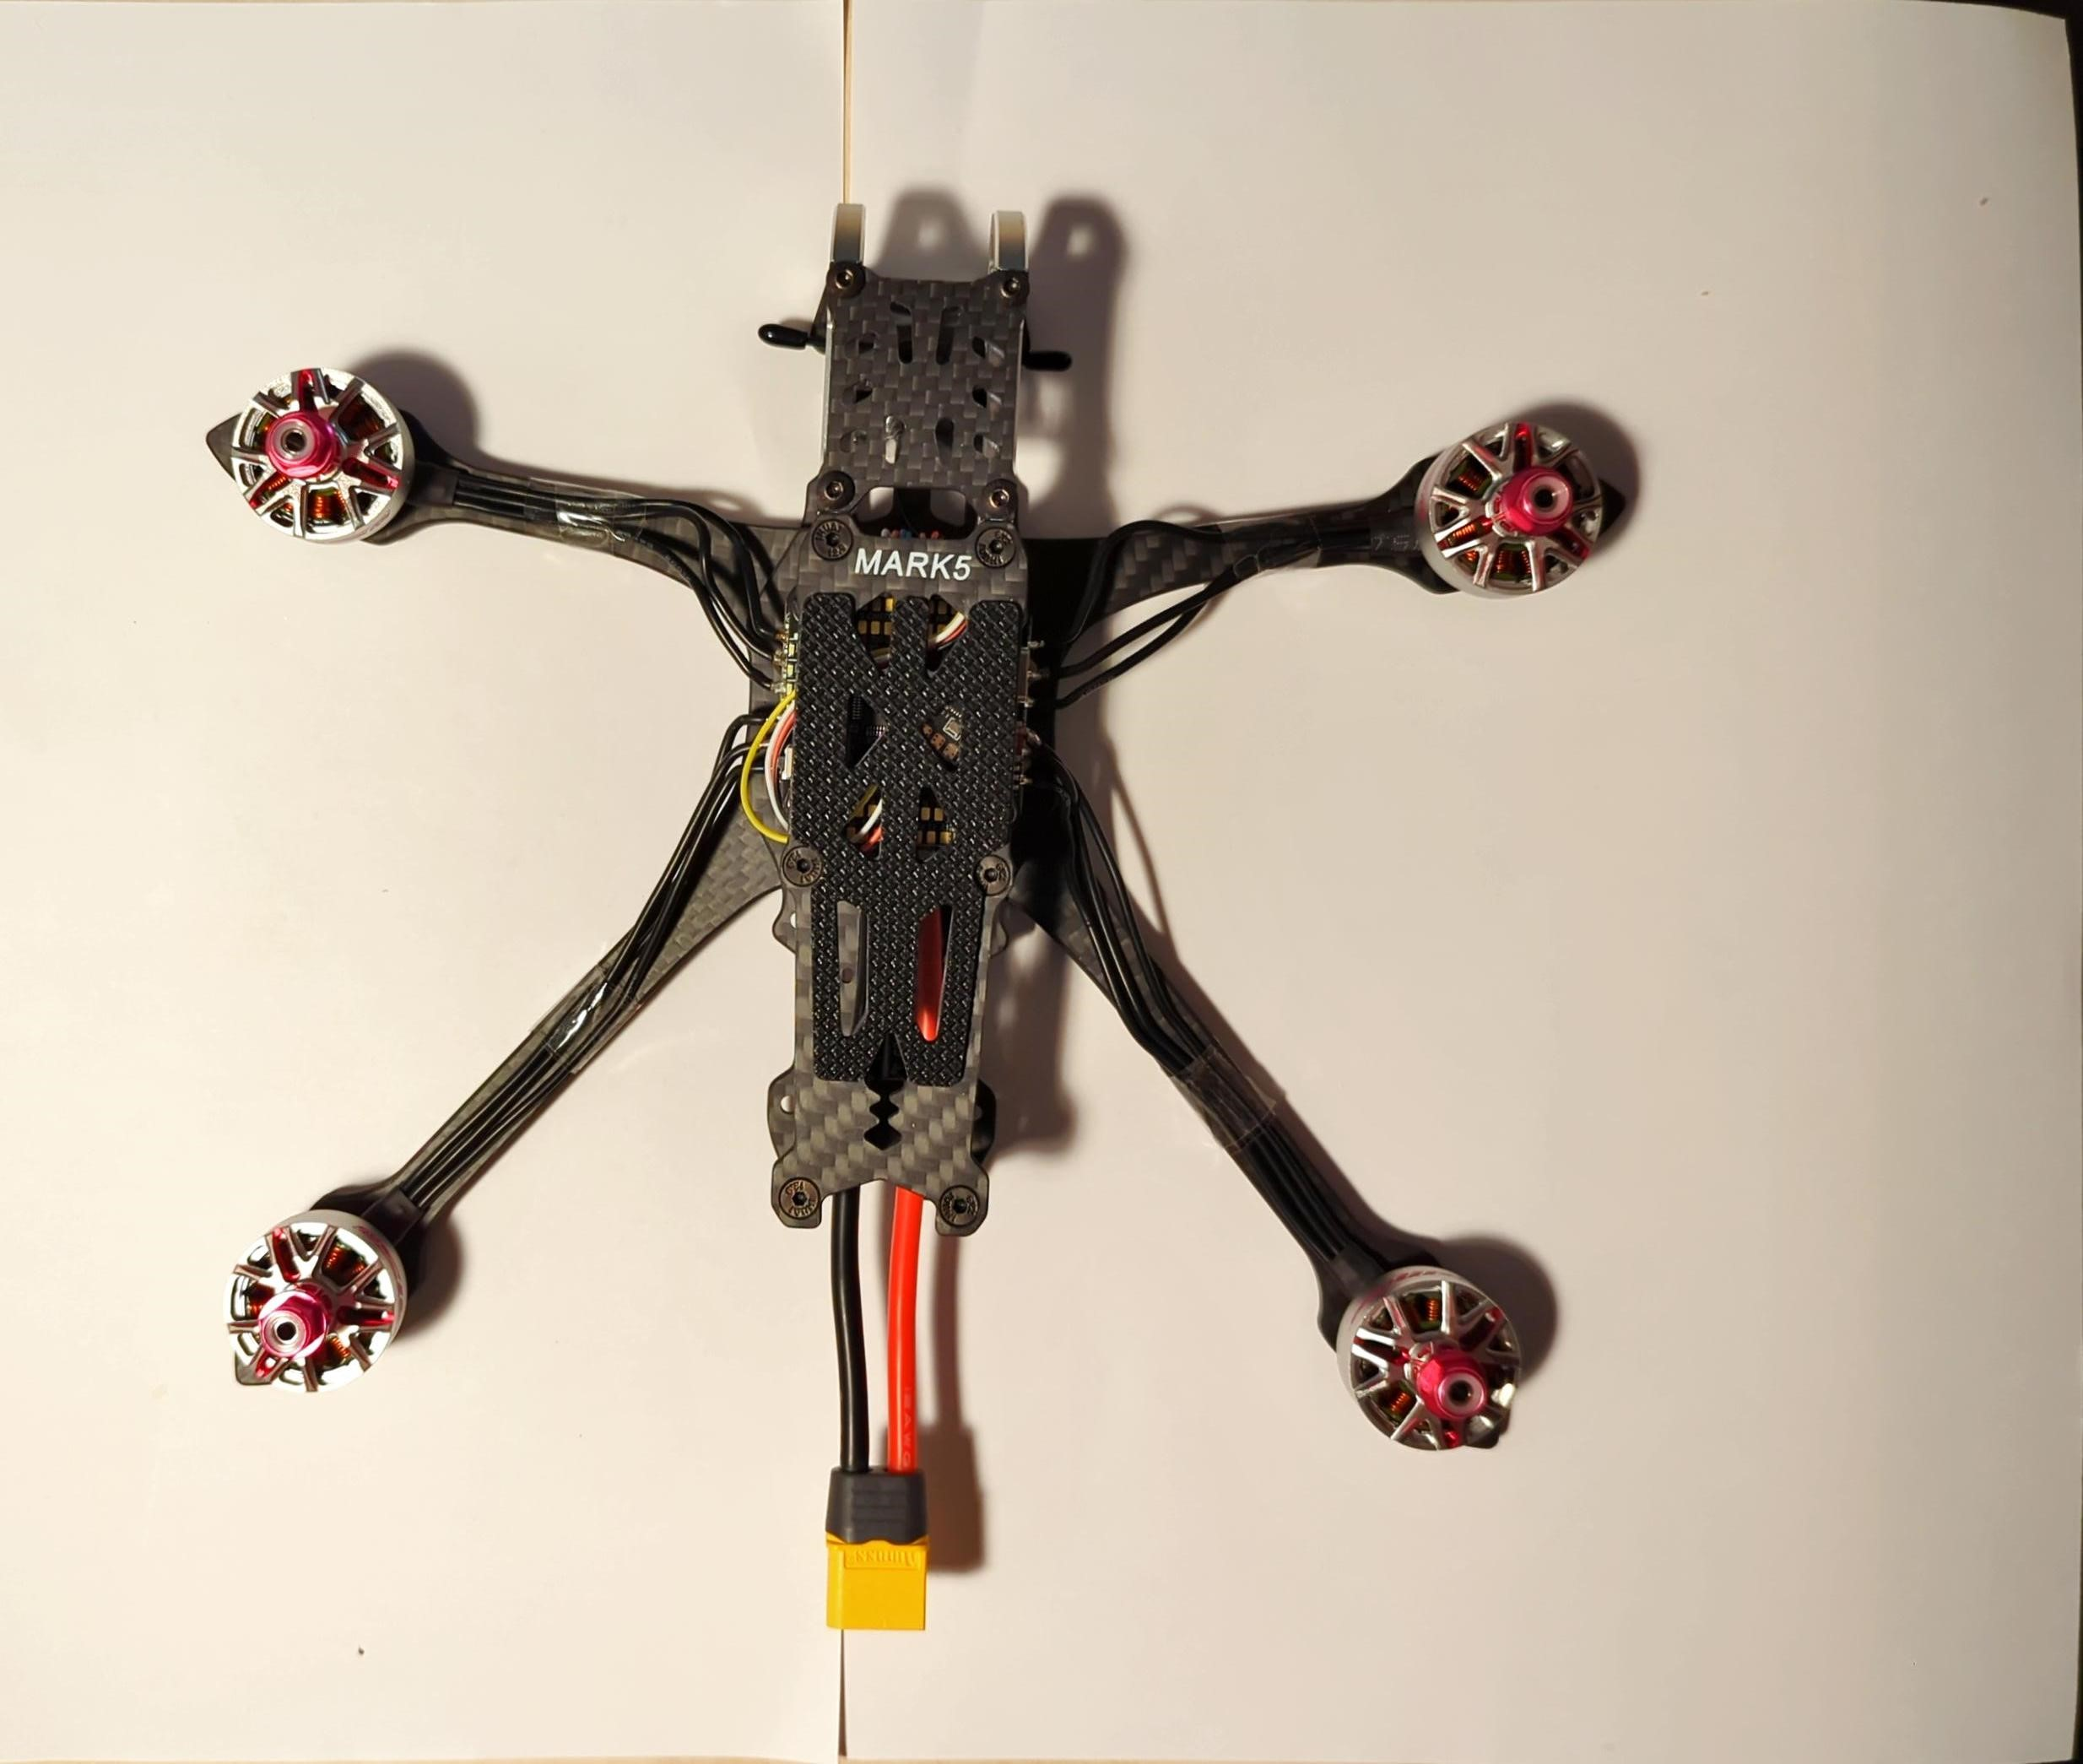
\includegraphics[width=\textwidth]{aufbaubilder/2024_04_06 12_00 Office Lens.jpg}
		\caption{Draufsicht auf die Drohe (ohne Propeller und Akku).}
		\label{fig:aufbau1}
	\end{minipage}%
	\hfill
	\begin{minipage}[b]{0.3\textwidth}
		\centering
		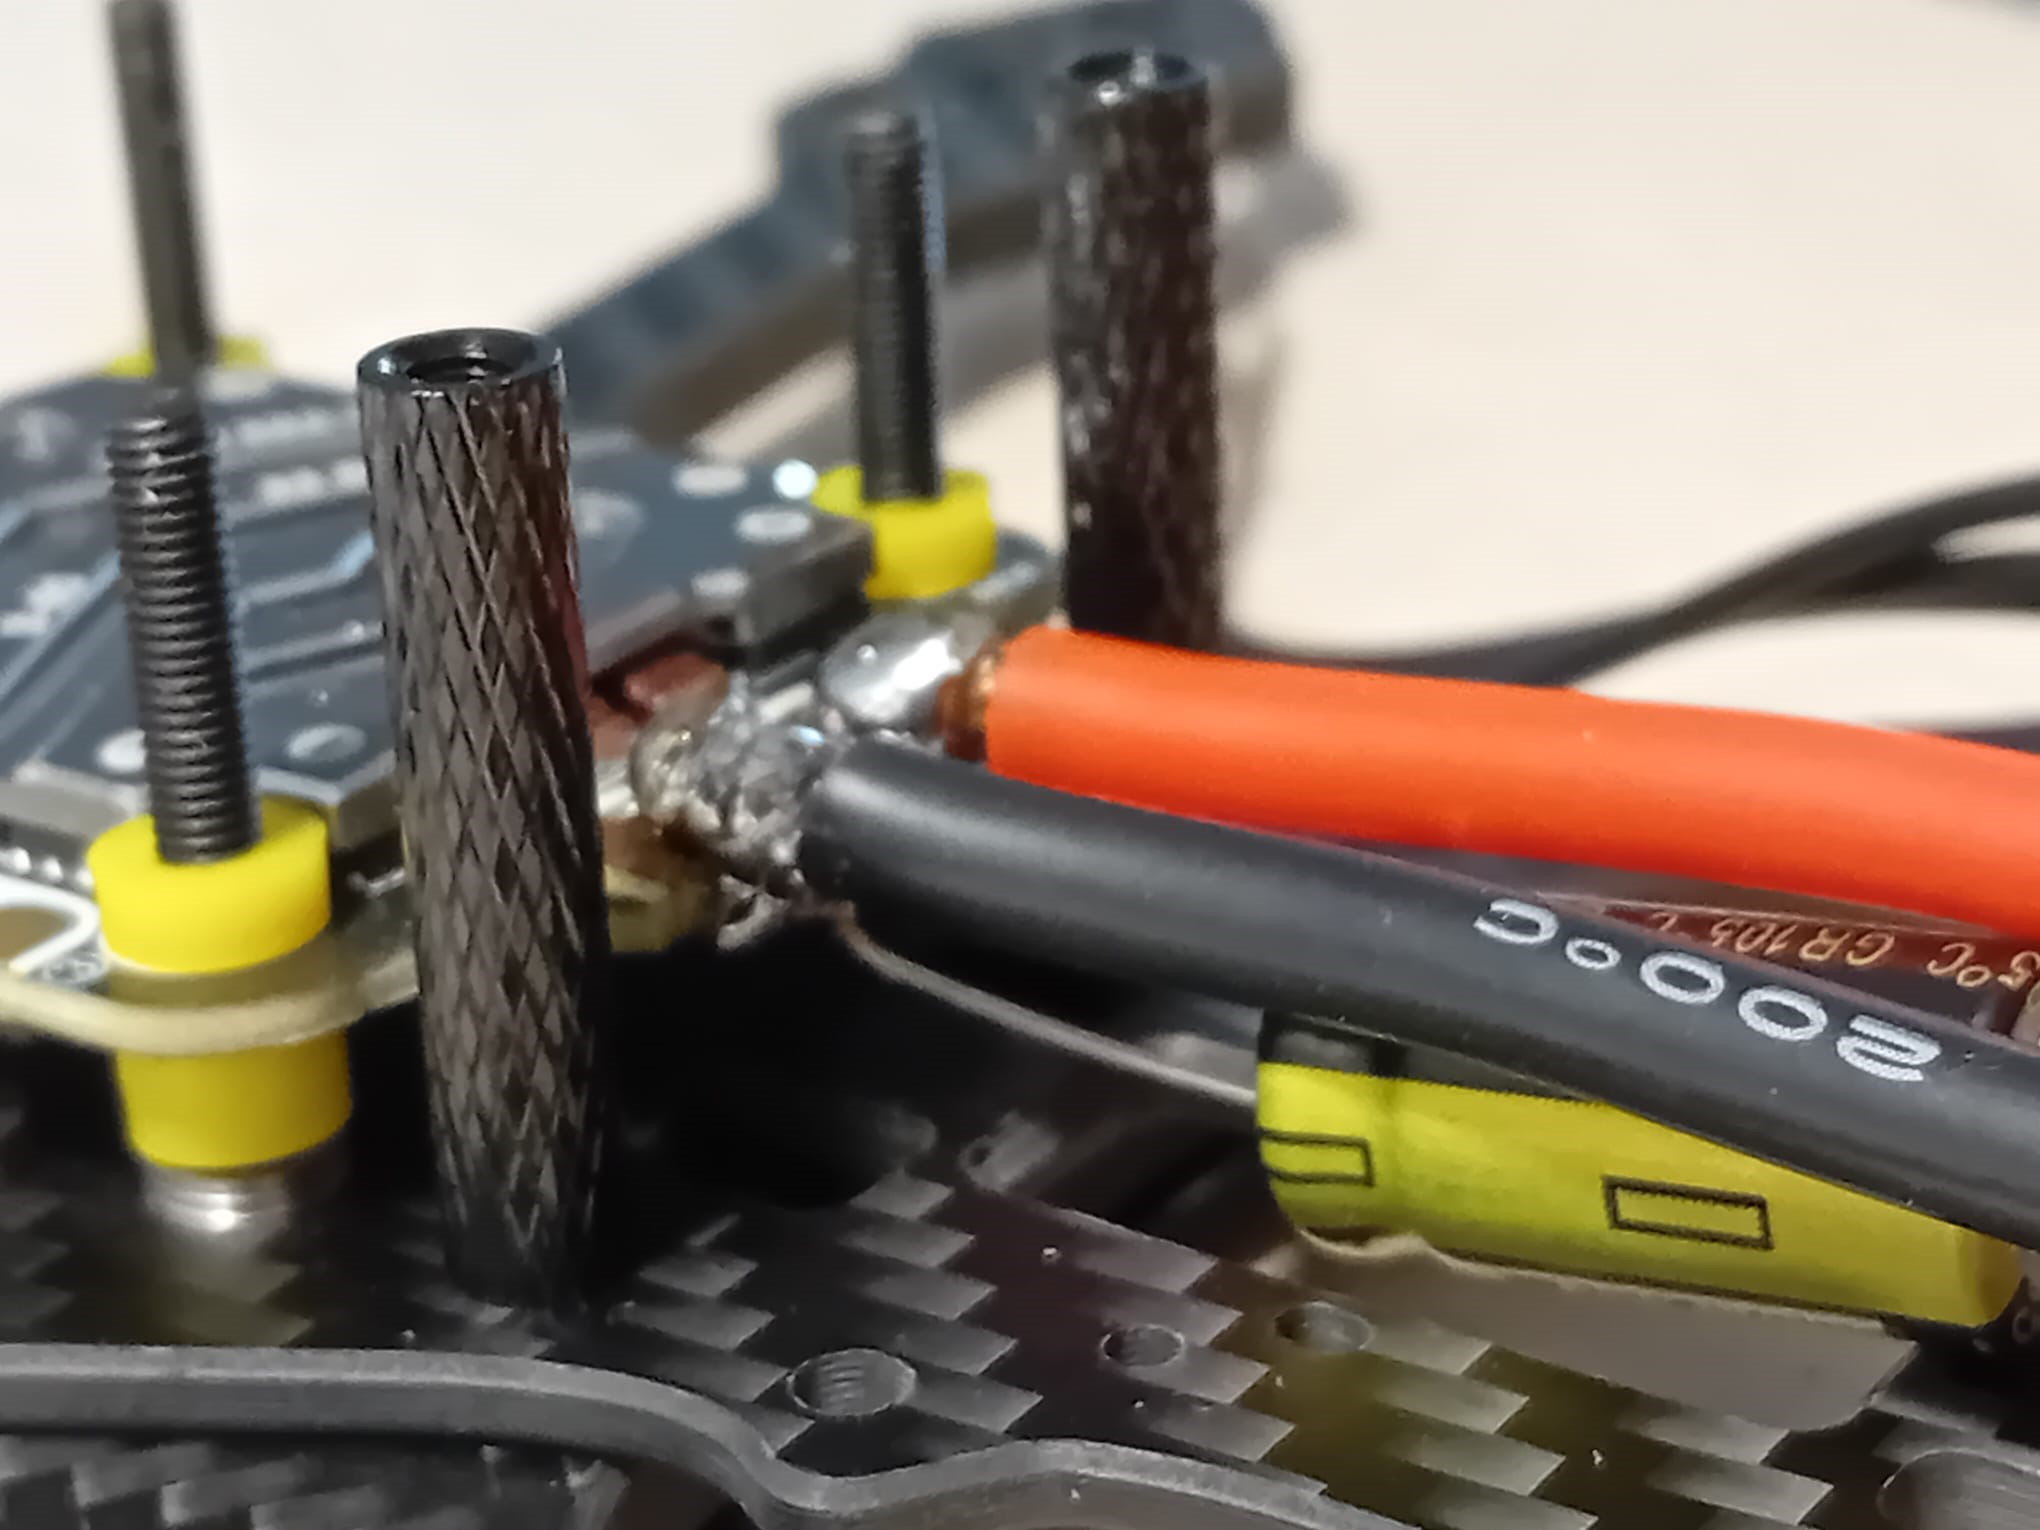
\includegraphics[width=\textwidth]{aufbaubilder/IMG-20240406-WA0012.jpg}
		\caption{Detailbild der Lötstelle Hauptstromversorgung mit Kondensator.}
		\label{fig:aufbau2}
	\end{minipage}%
	\hfill
	\begin{minipage}[b]{0.3\textwidth}
		\centering
		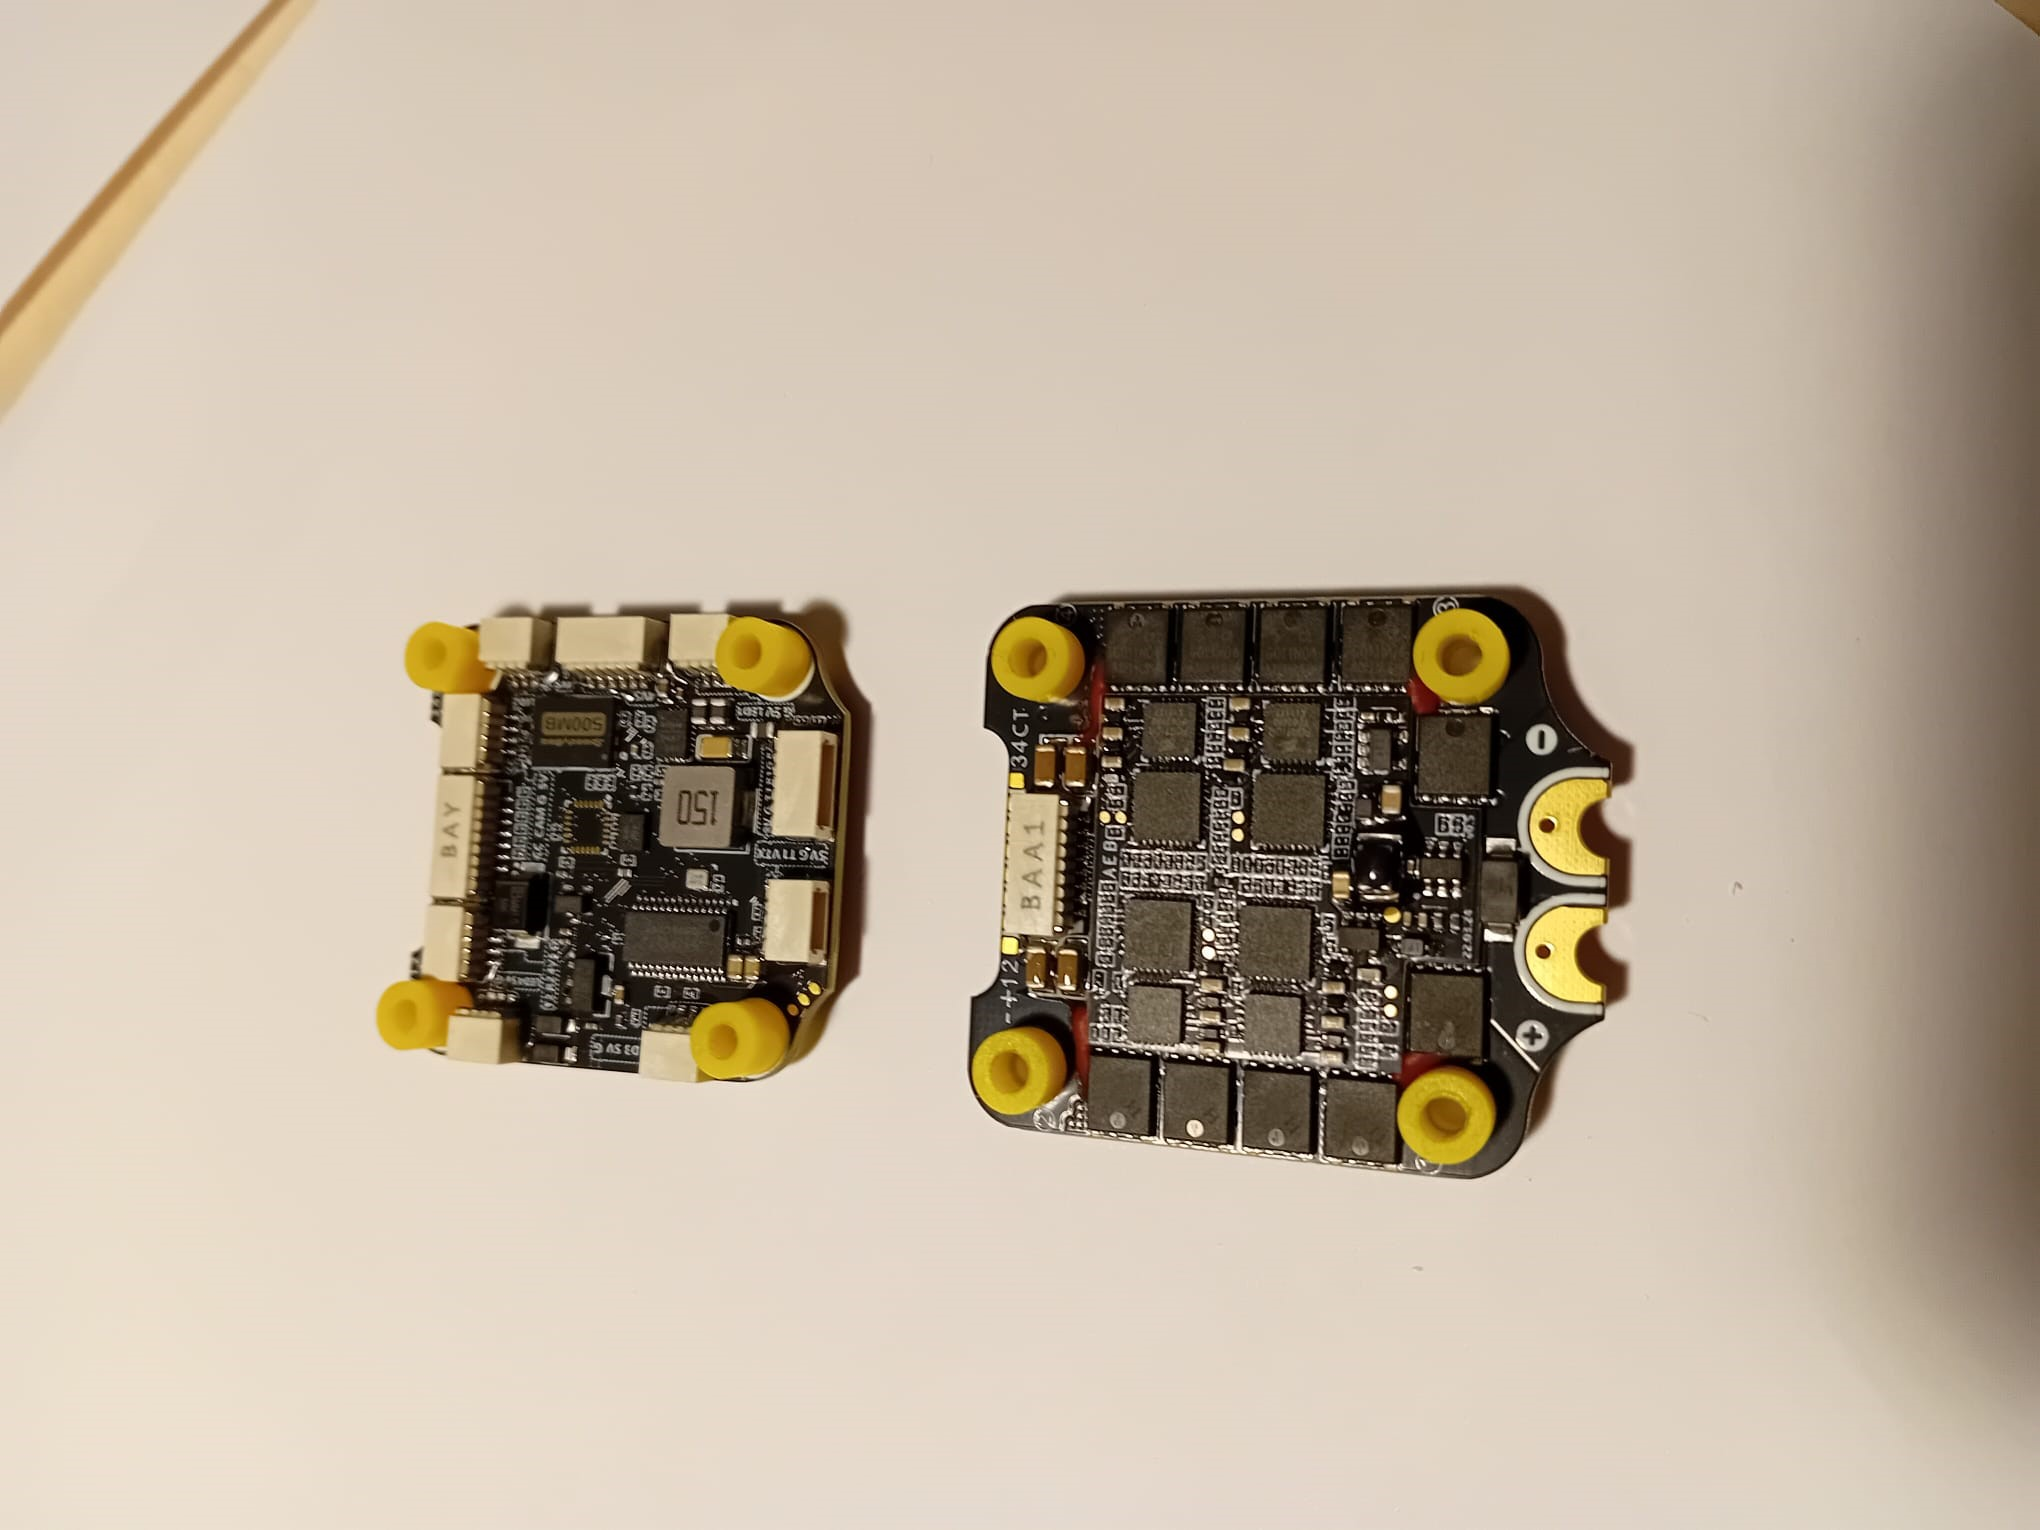
\includegraphics[width=\textwidth]{aufbaubilder/IMG-20240406-WA0014.jpg}
		\caption{Ansicht auf ESC und FC}
		\label{fig:aufbau3}
	\end{minipage}

	\vskip 0.5cm % Abstand zwischen den Reihen
\end{figure}
\begin{figure}[htbp]	
	% Zweite Reihe mit drei Bildern
	\begin{minipage}[b]{0.3\textwidth}
		\centering
		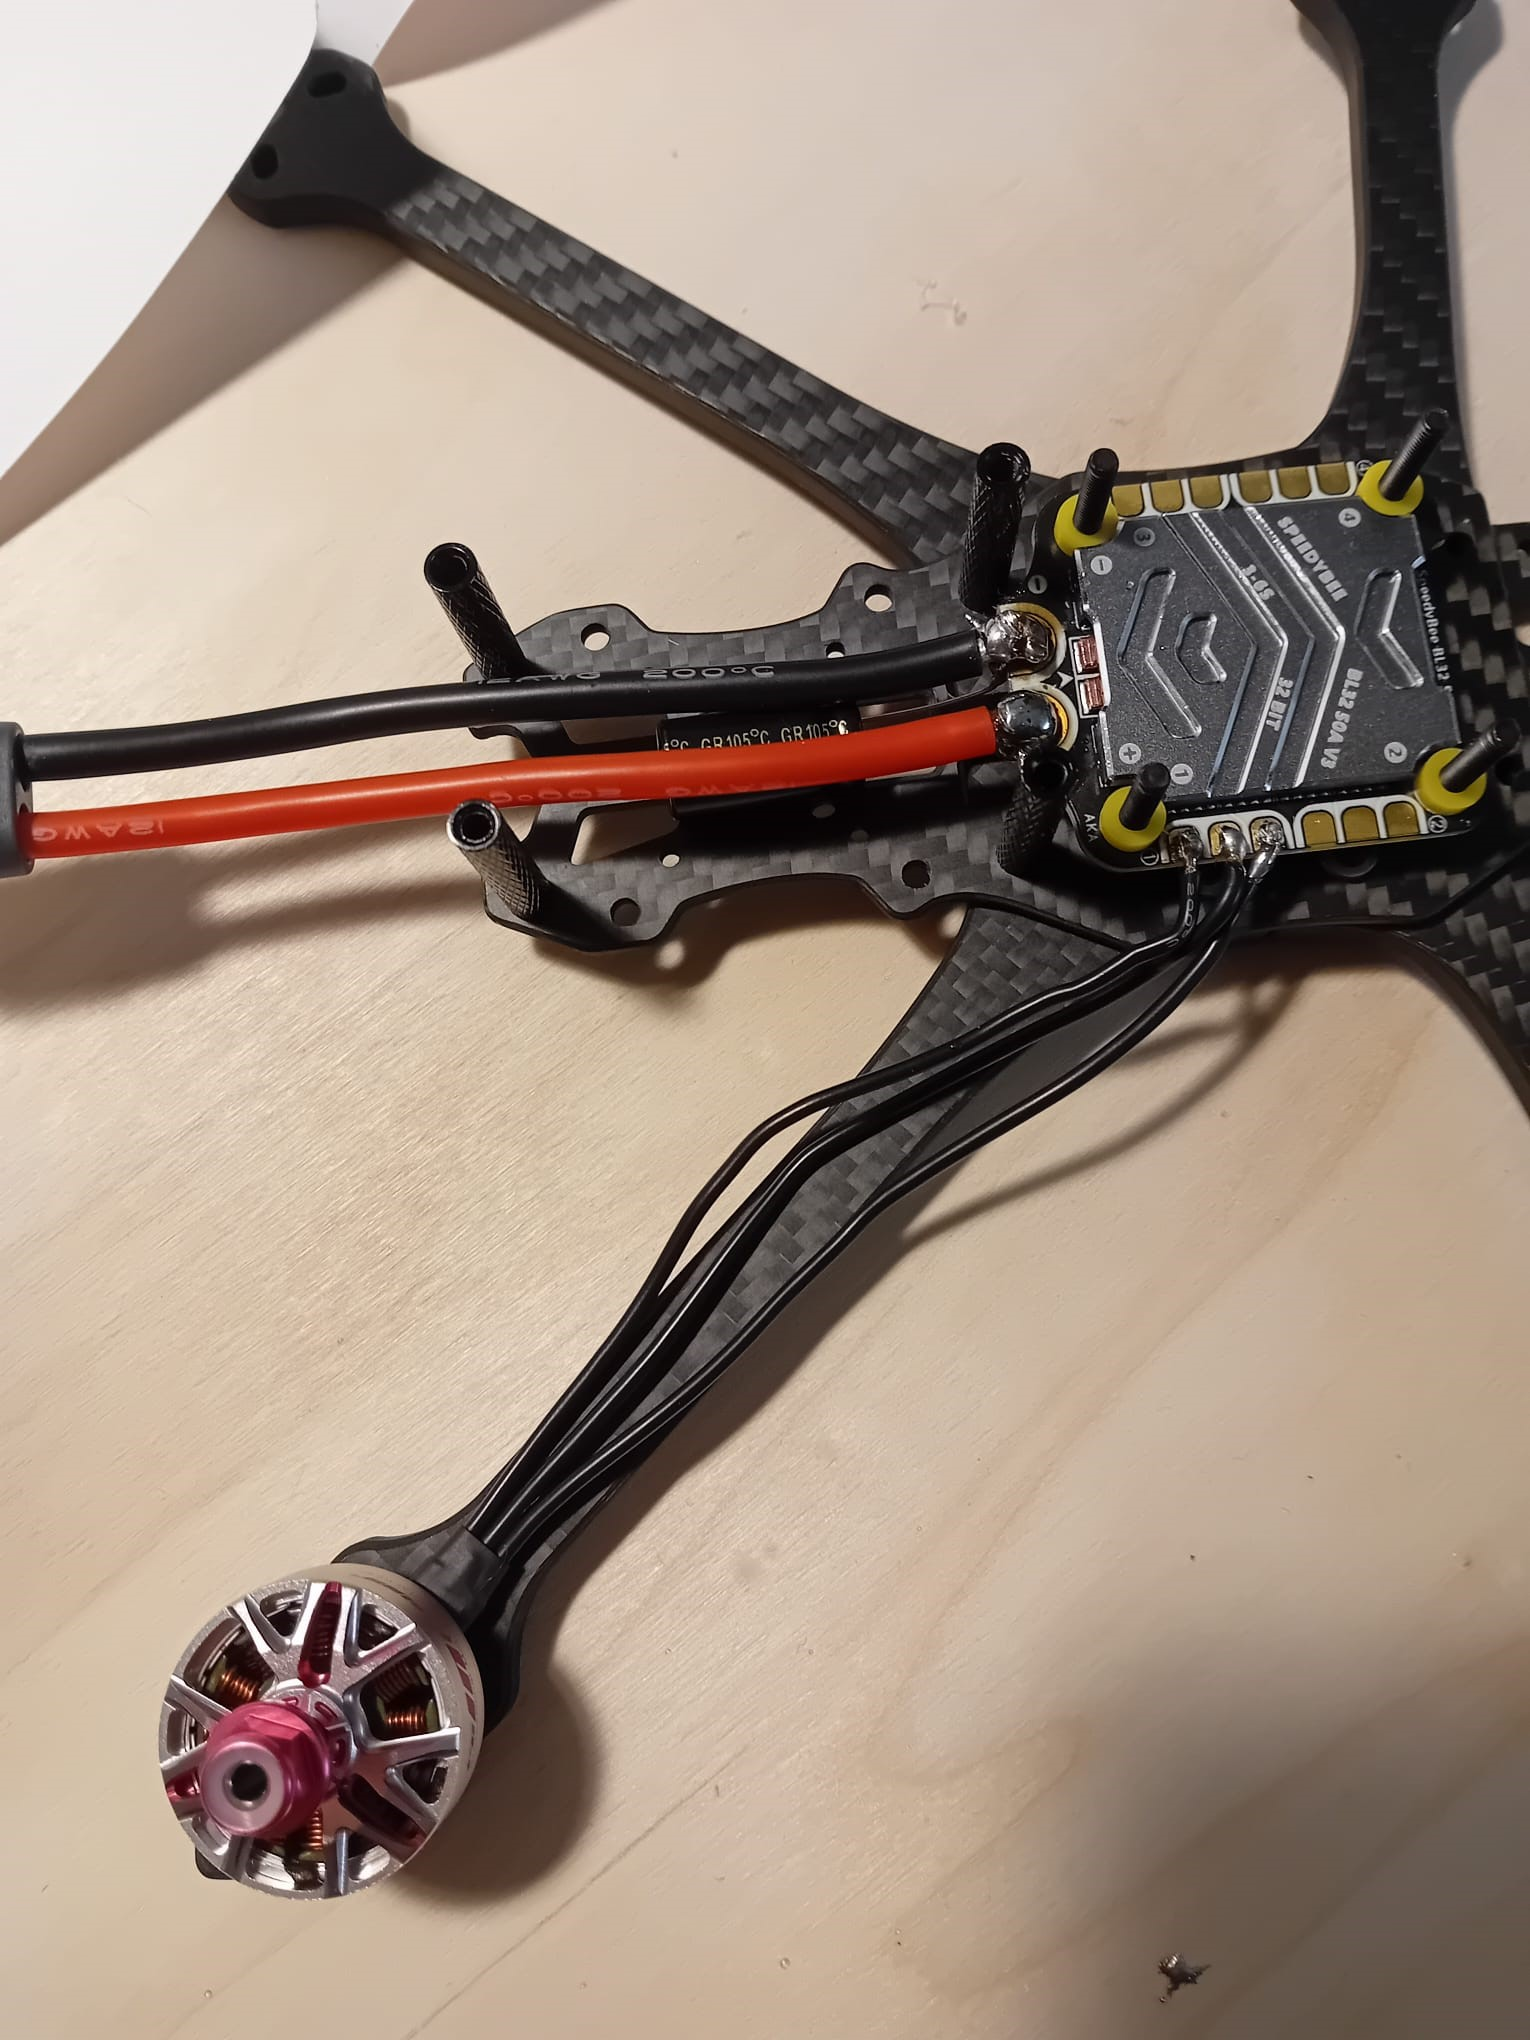
\includegraphics[width=\textwidth]{aufbaubilder/IMG-20240406-WA0009.jpg}
		\caption{Drohen mit erstem Motor angelötet.}
		\label{fig:aufbau4}
	\end{minipage}%
	\hfill
	\begin{minipage}[b]{0.3\textwidth}
		\centering
		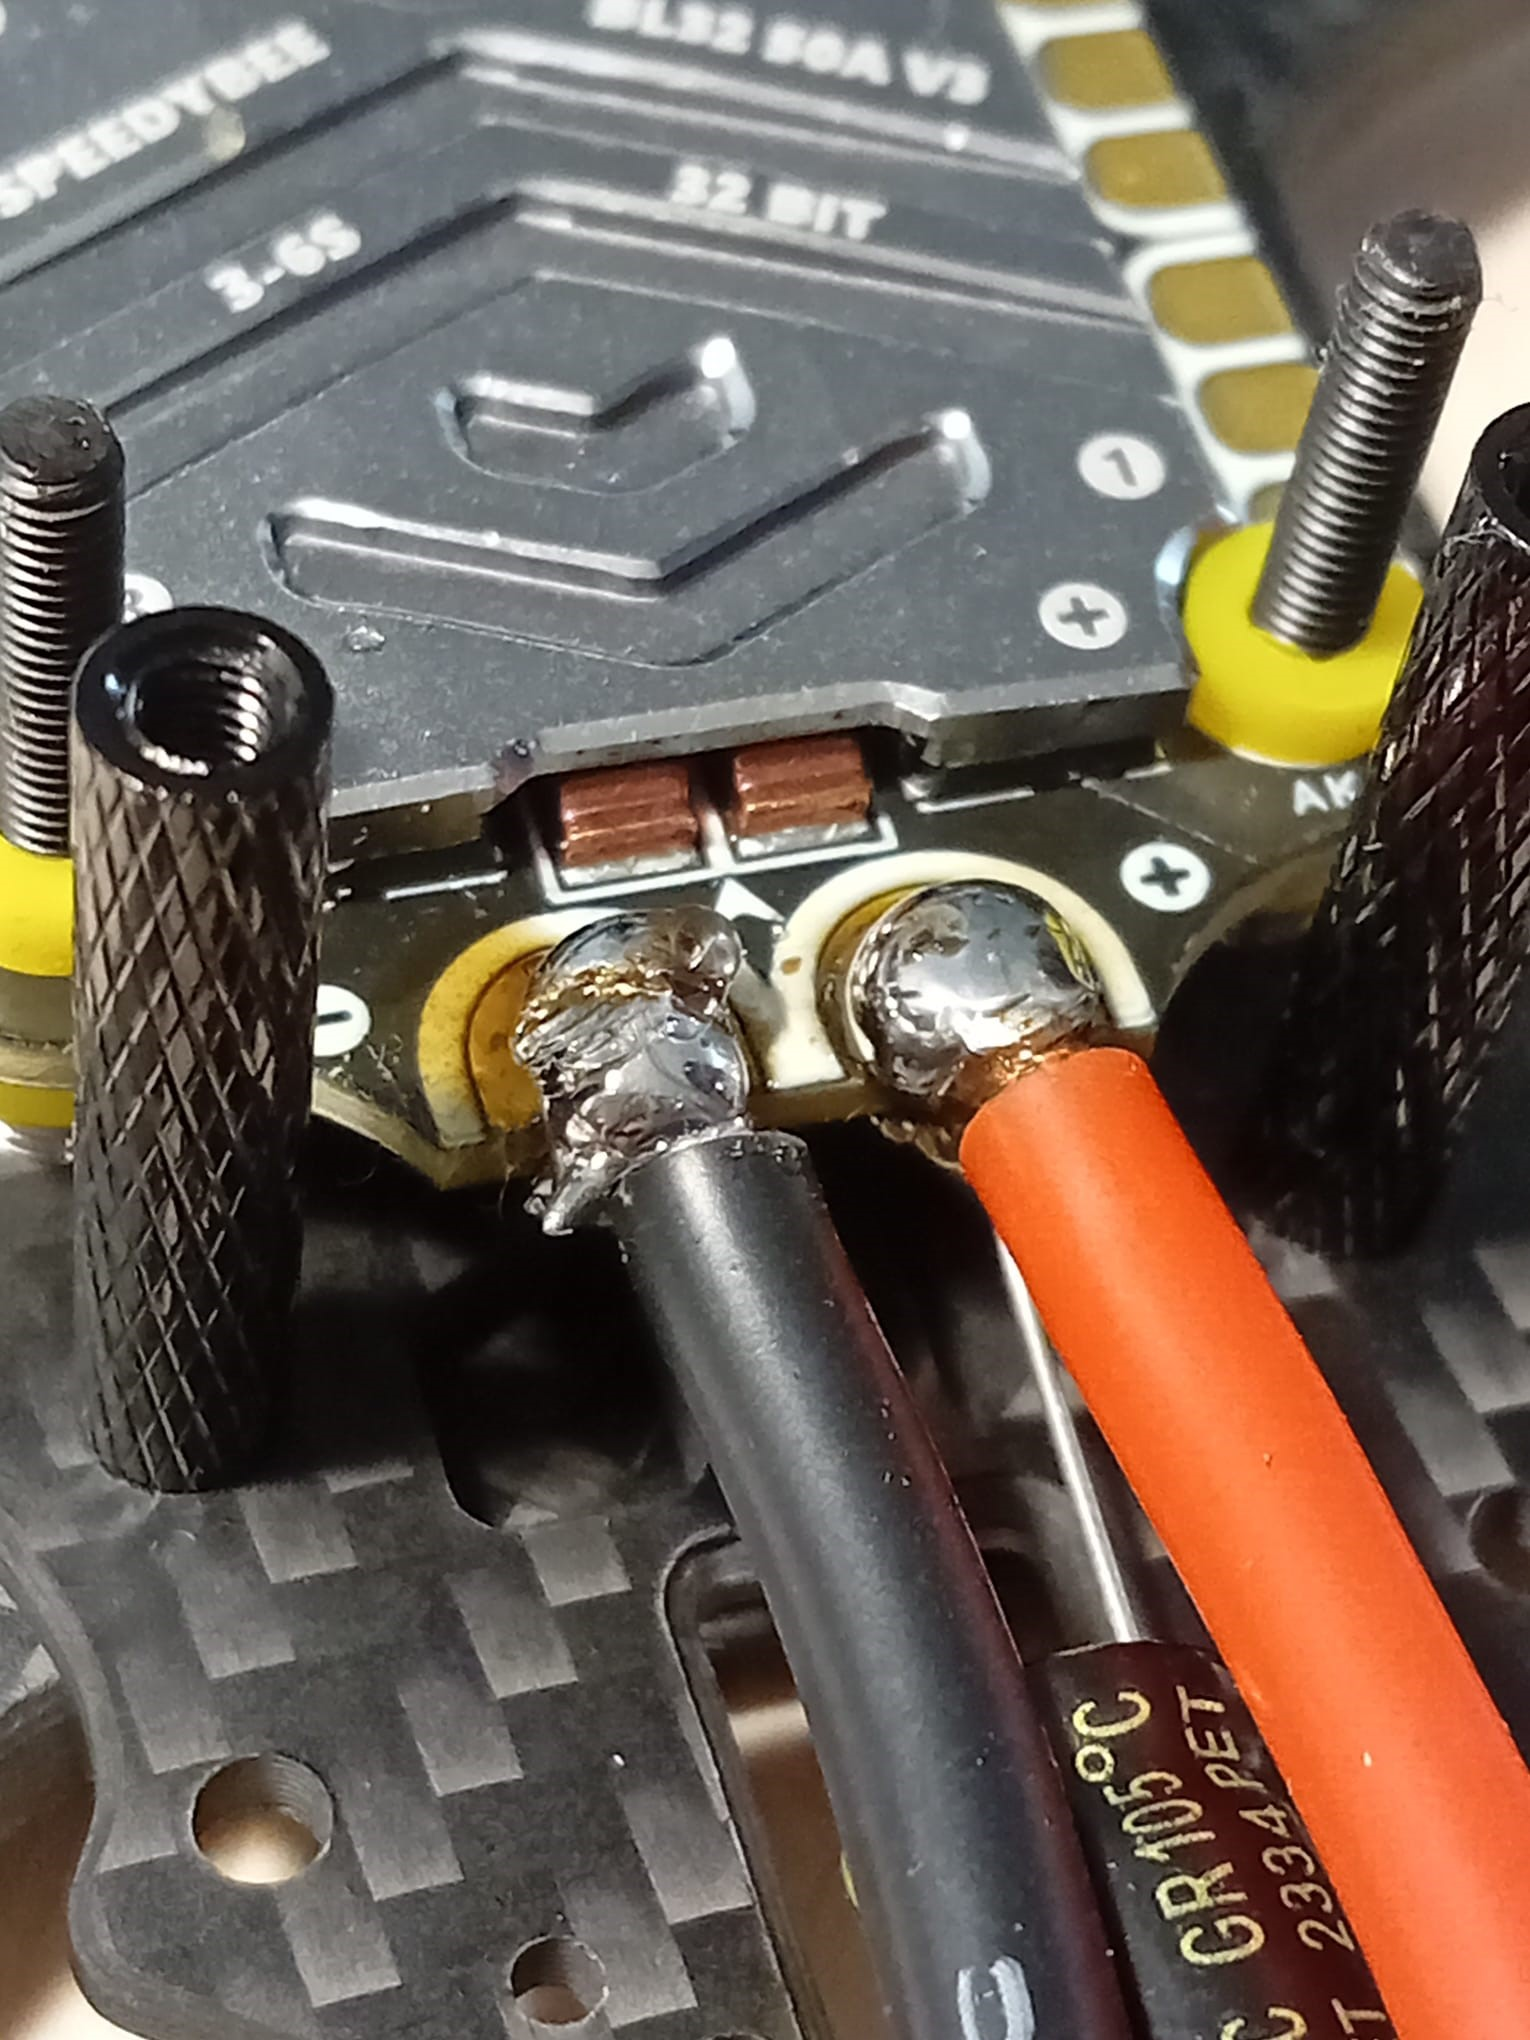
\includegraphics[width=\textwidth]{aufbaubilder/IMG-20240406-WA0013.jpg}
		\caption{Nahaufnahme der Hauptstromversorgung mit Kondensator.}
		\label{fig:aufbau5}
	\end{minipage}%
	\hfill
	\begin{minipage}[b]{0.3\textwidth}
		\centering
		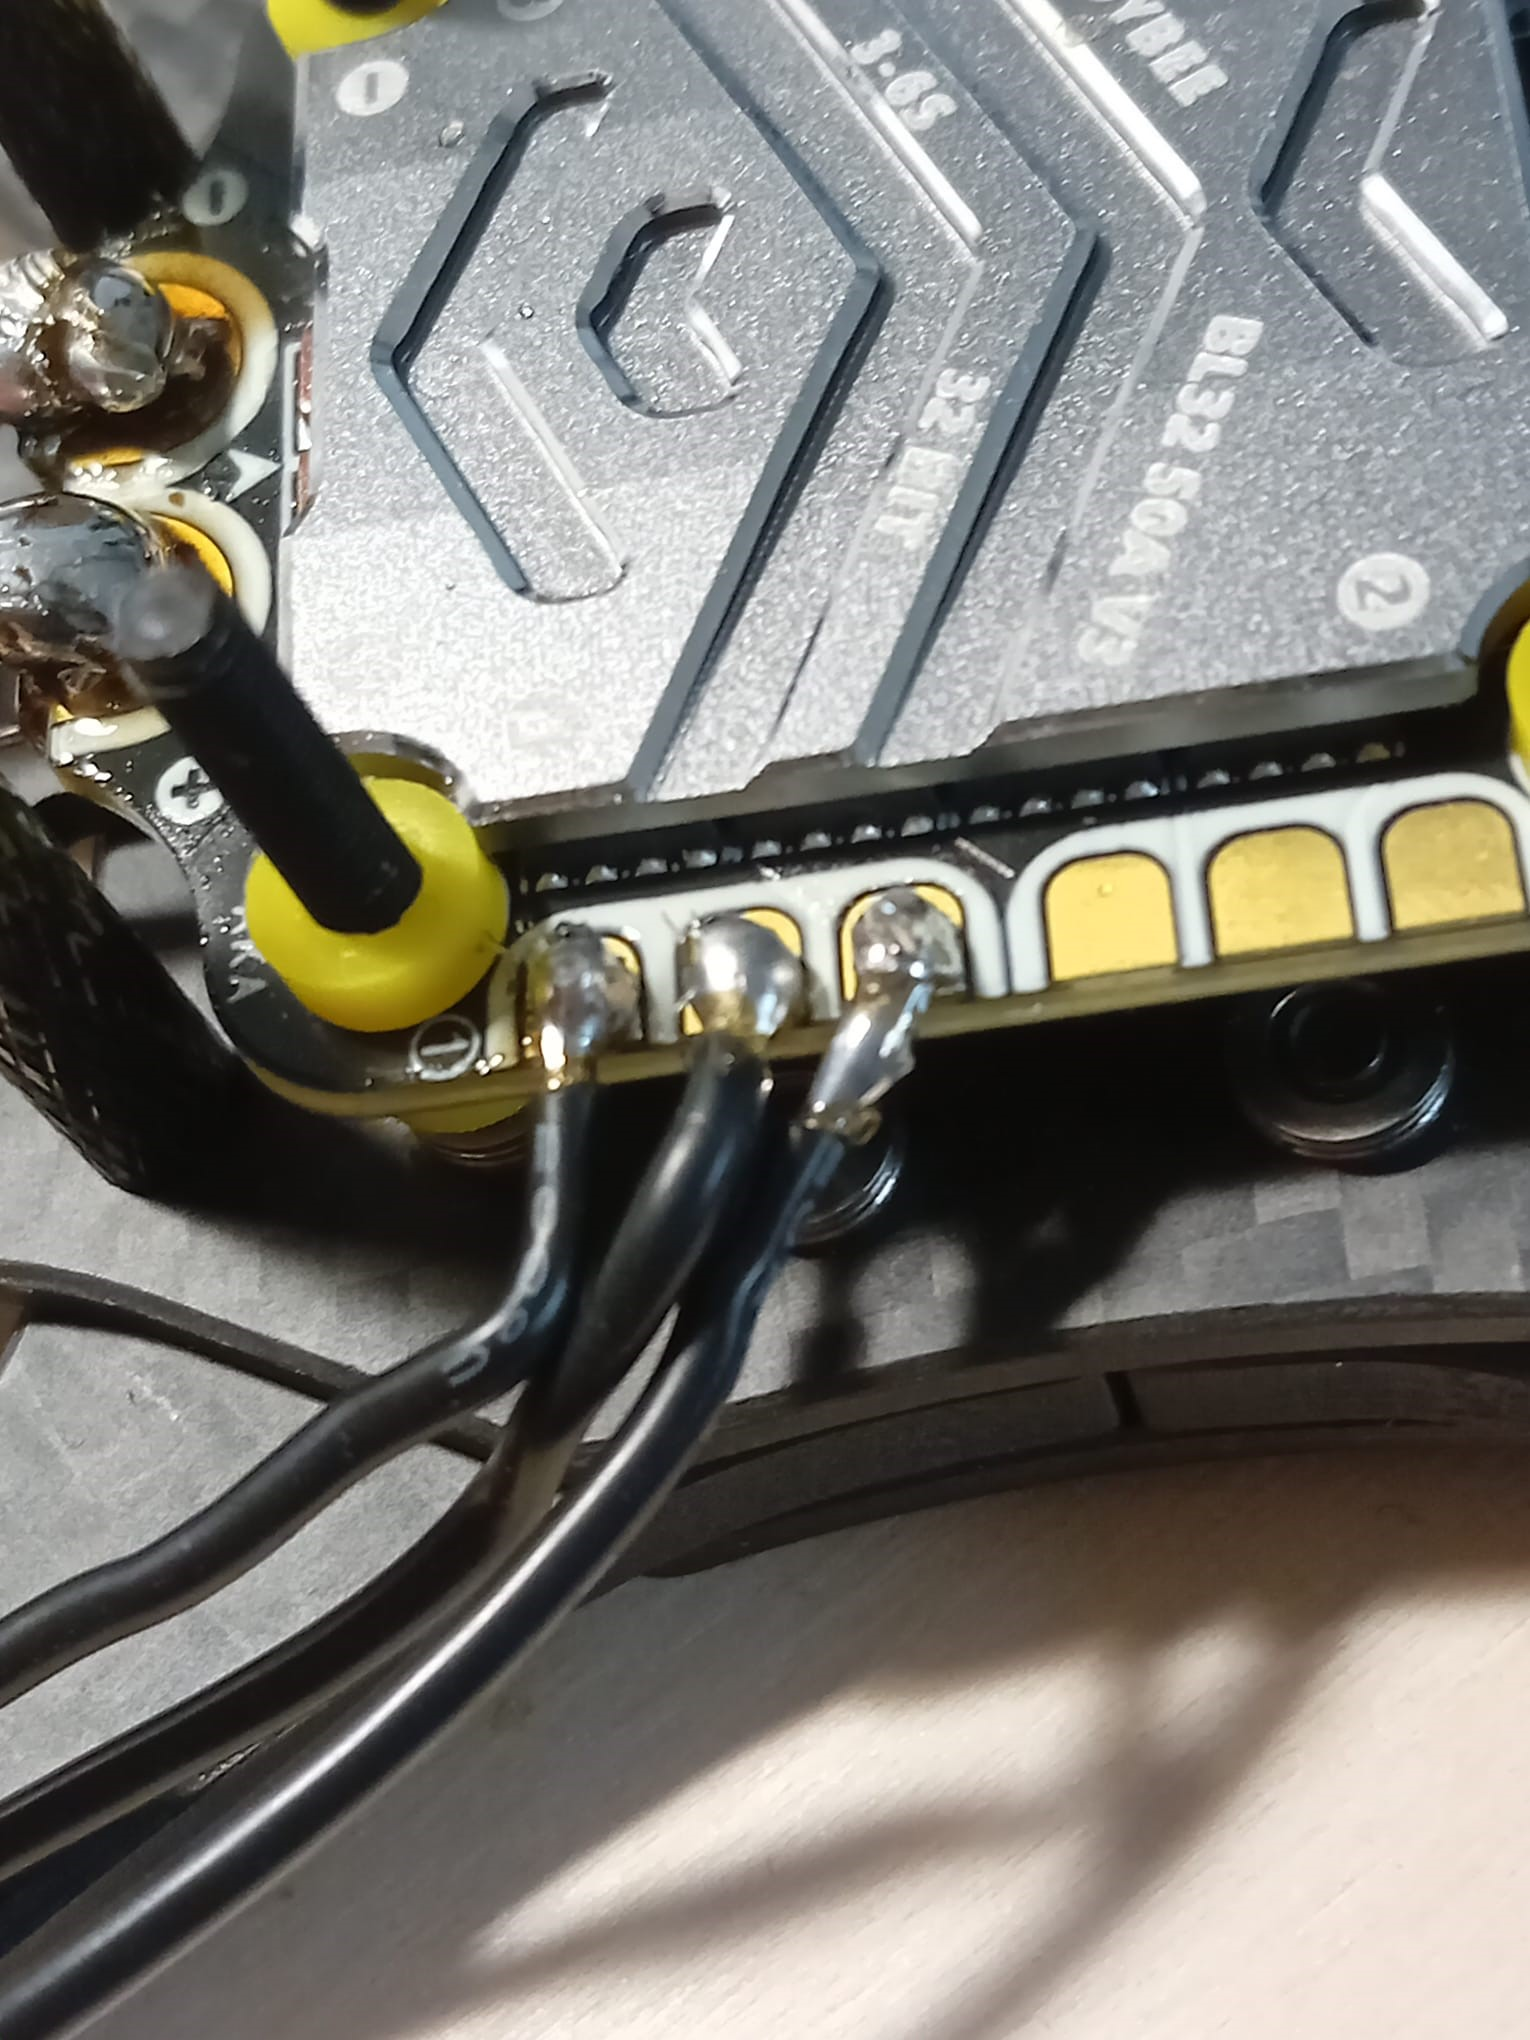
\includegraphics[width=\textwidth]{aufbaubilder/IMG-20240406-WA0011.jpg}
		\caption{Nahaufnahme vom ersten angelöteten Motorkabel.}
		\label{fig:aufbau6}
	\end{minipage}
	
	\vskip 0.5cm % Abstand zwischen den Reihen
\end{figure}
\begin{figure}[htbp]
	% Dritte Reihe mit drei Bildern
	\begin{minipage}[b]{0.3\textwidth}
		\centering
		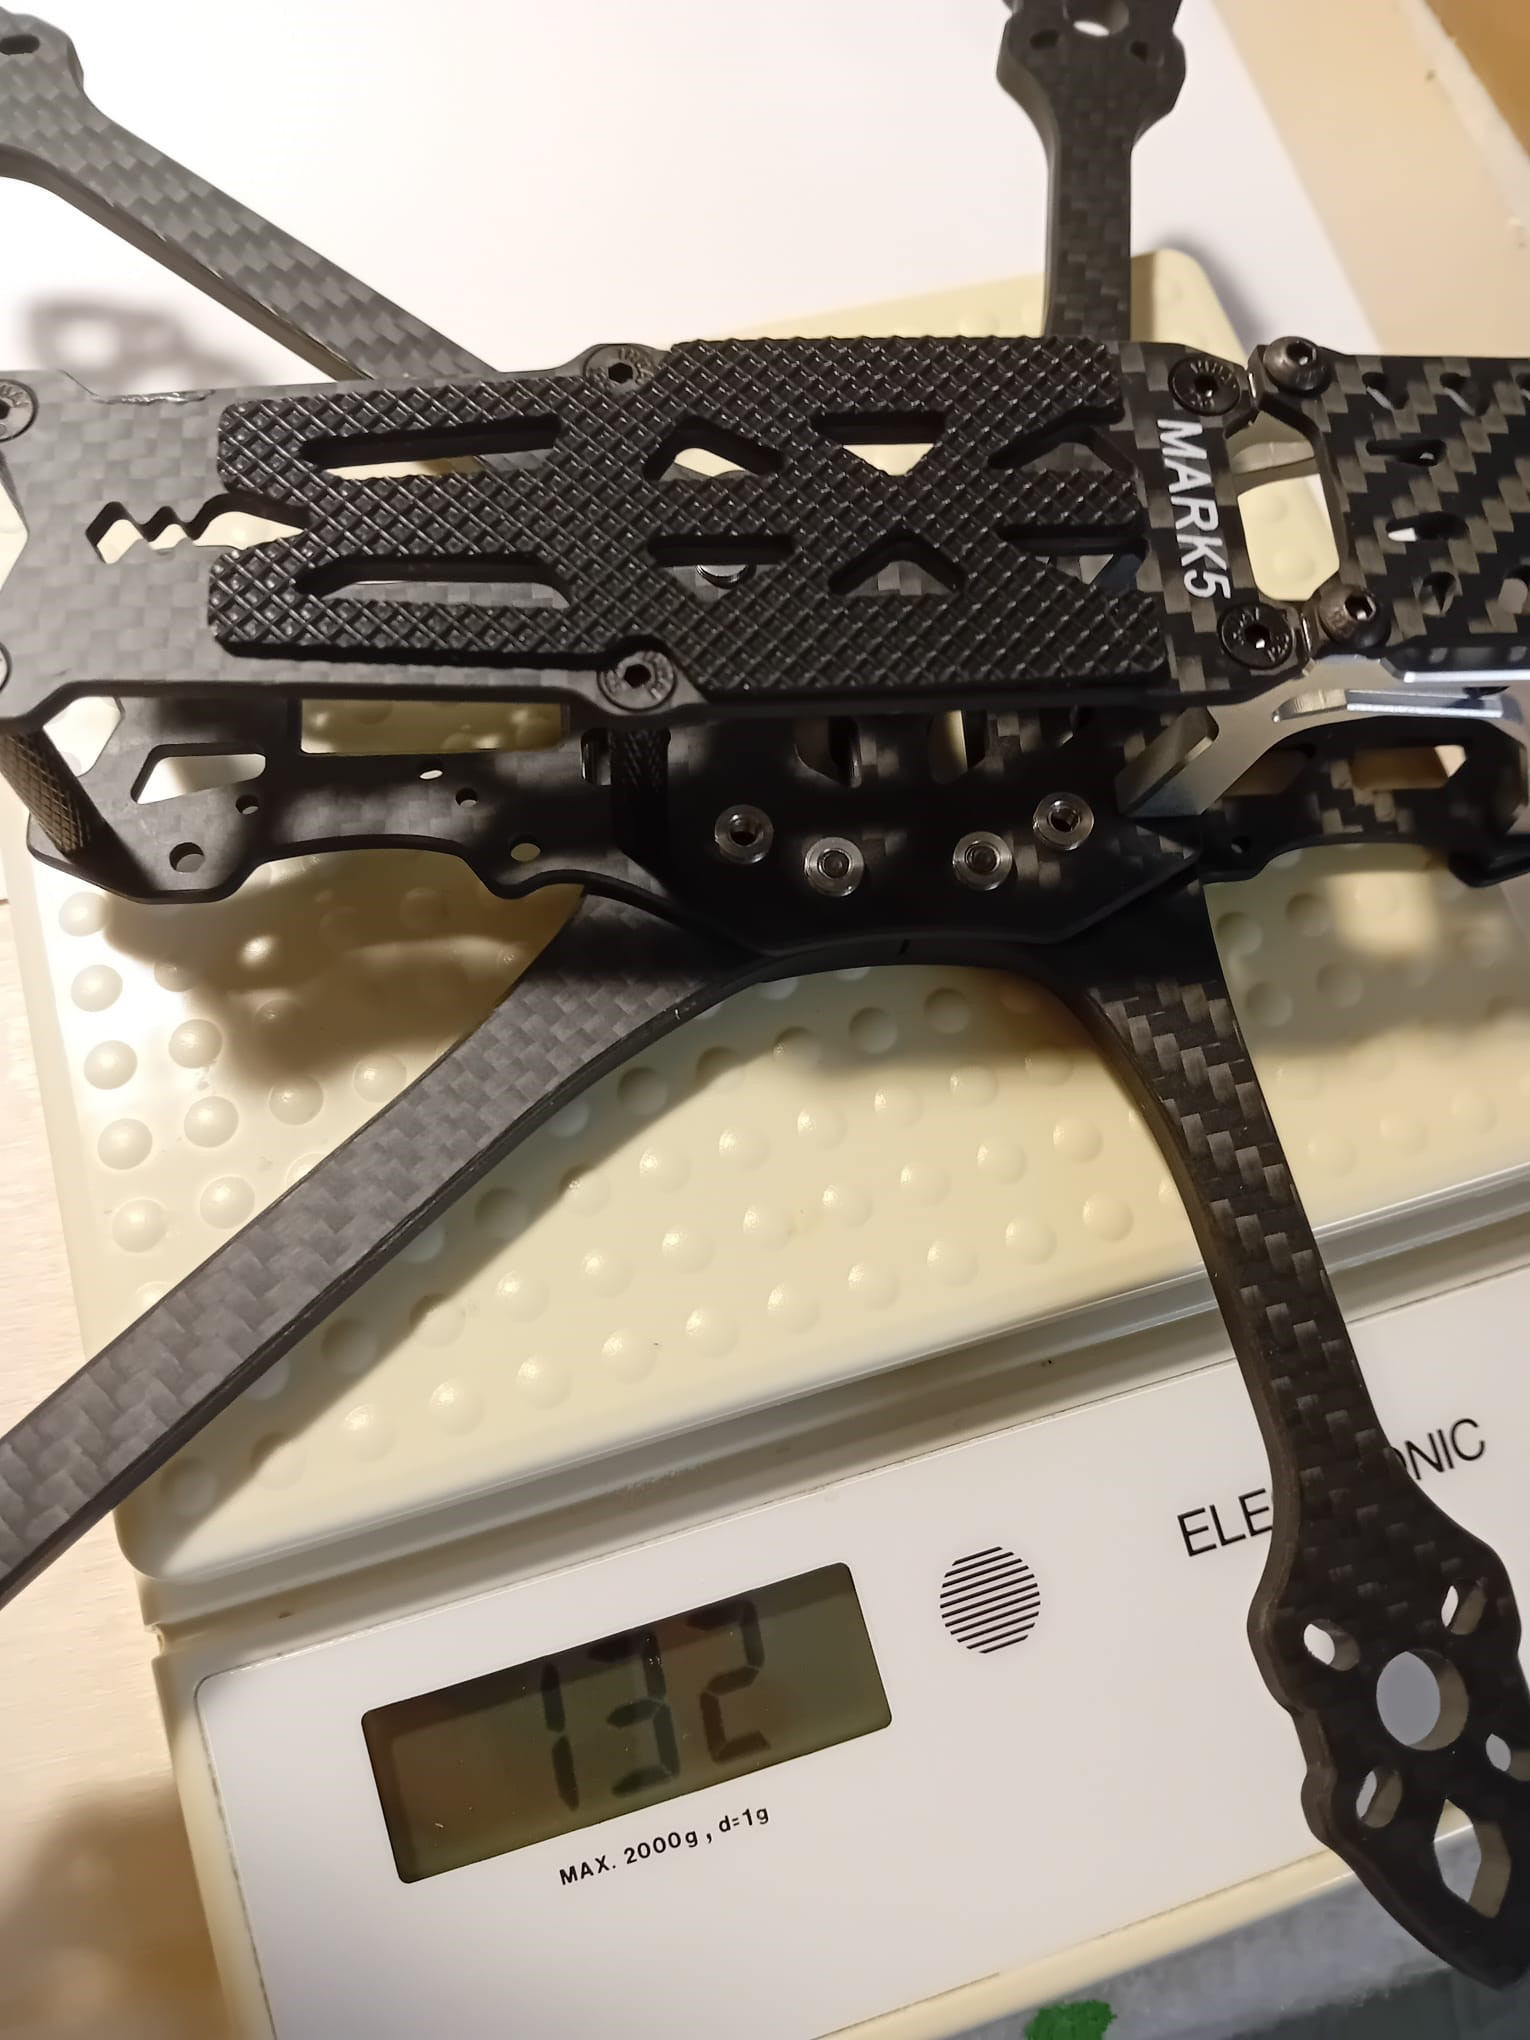
\includegraphics[width=\textwidth]{aufbaubilder/IMG-20240406-WA0015.jpg}
		\caption{Zusammengebauter Frame auf der Waage.}
		\label{fig:aufbau7}
	\end{minipage}%
	\hfill
	\begin{minipage}[b]{0.3\textwidth}
		\centering
		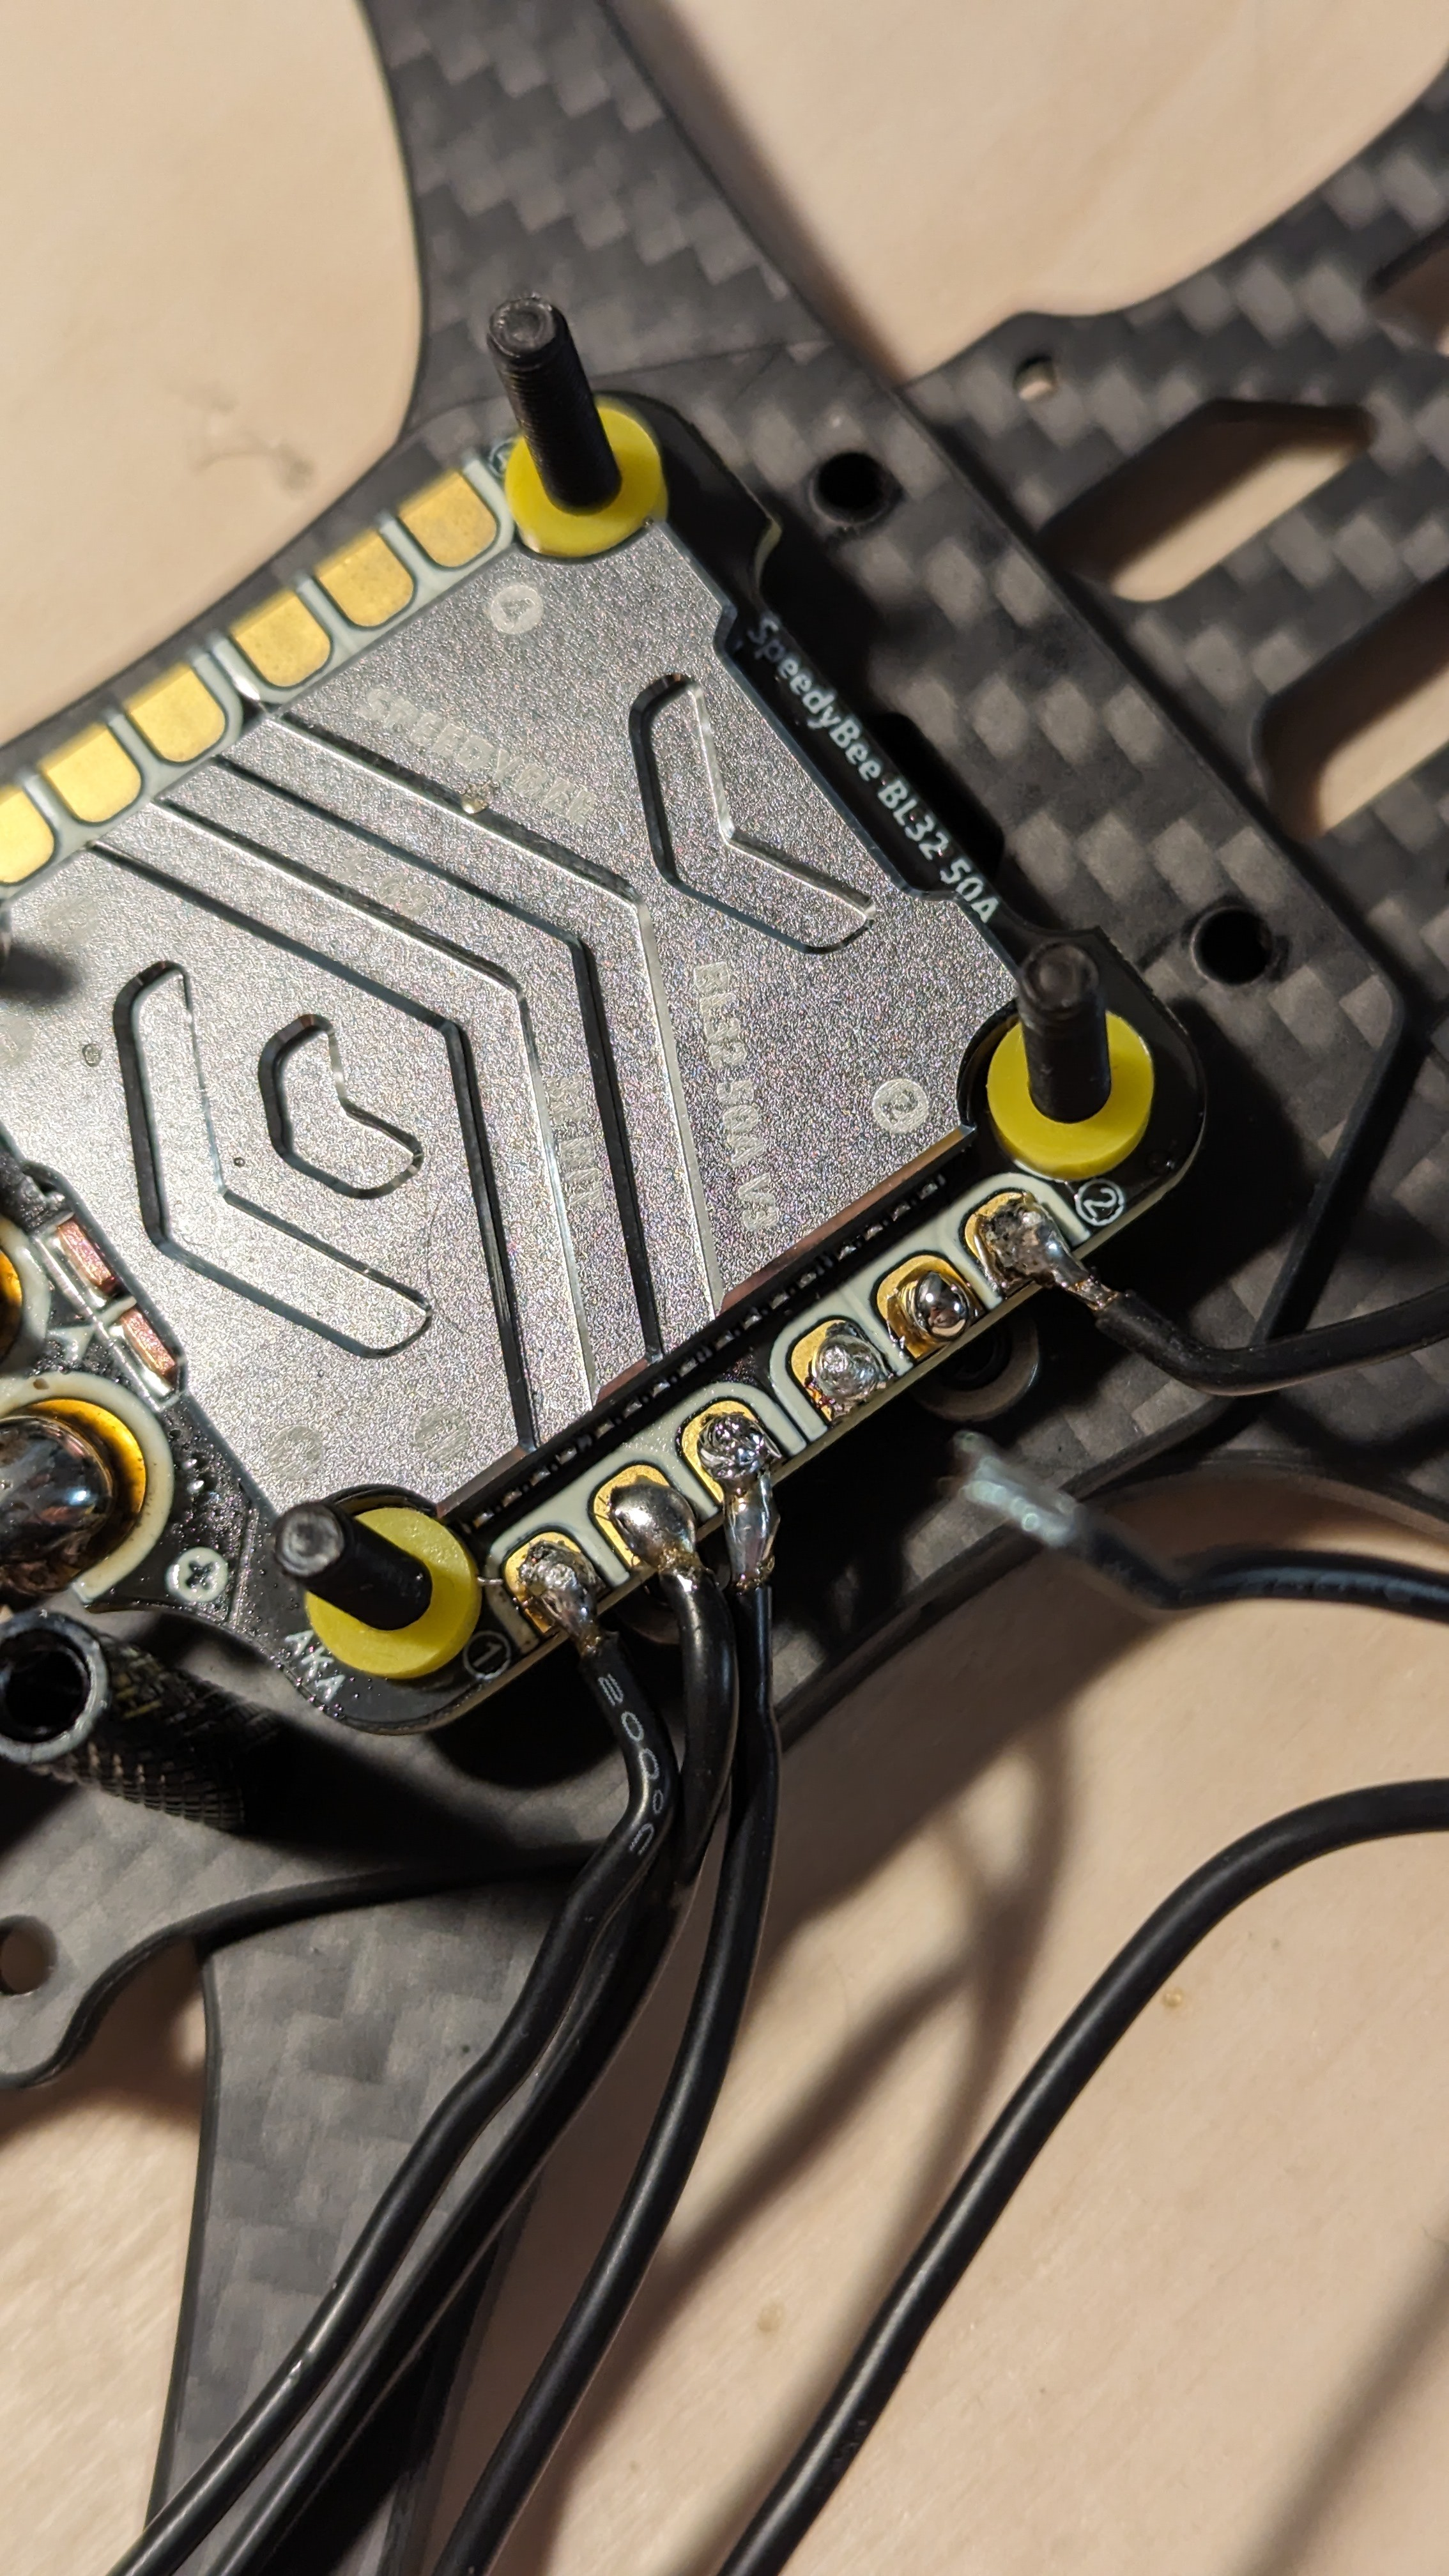
\includegraphics[width=\textwidth]{aufbaubilder/pro-oUIduoYj.jpeg}
		\caption{Fehlerhafte Lötstelle des zweiten Motors.}
		\label{fig:aufbau9}
	\end{minipage}%
	\hfill
	\begin{minipage}[b]{0.3\textwidth}
		\centering
		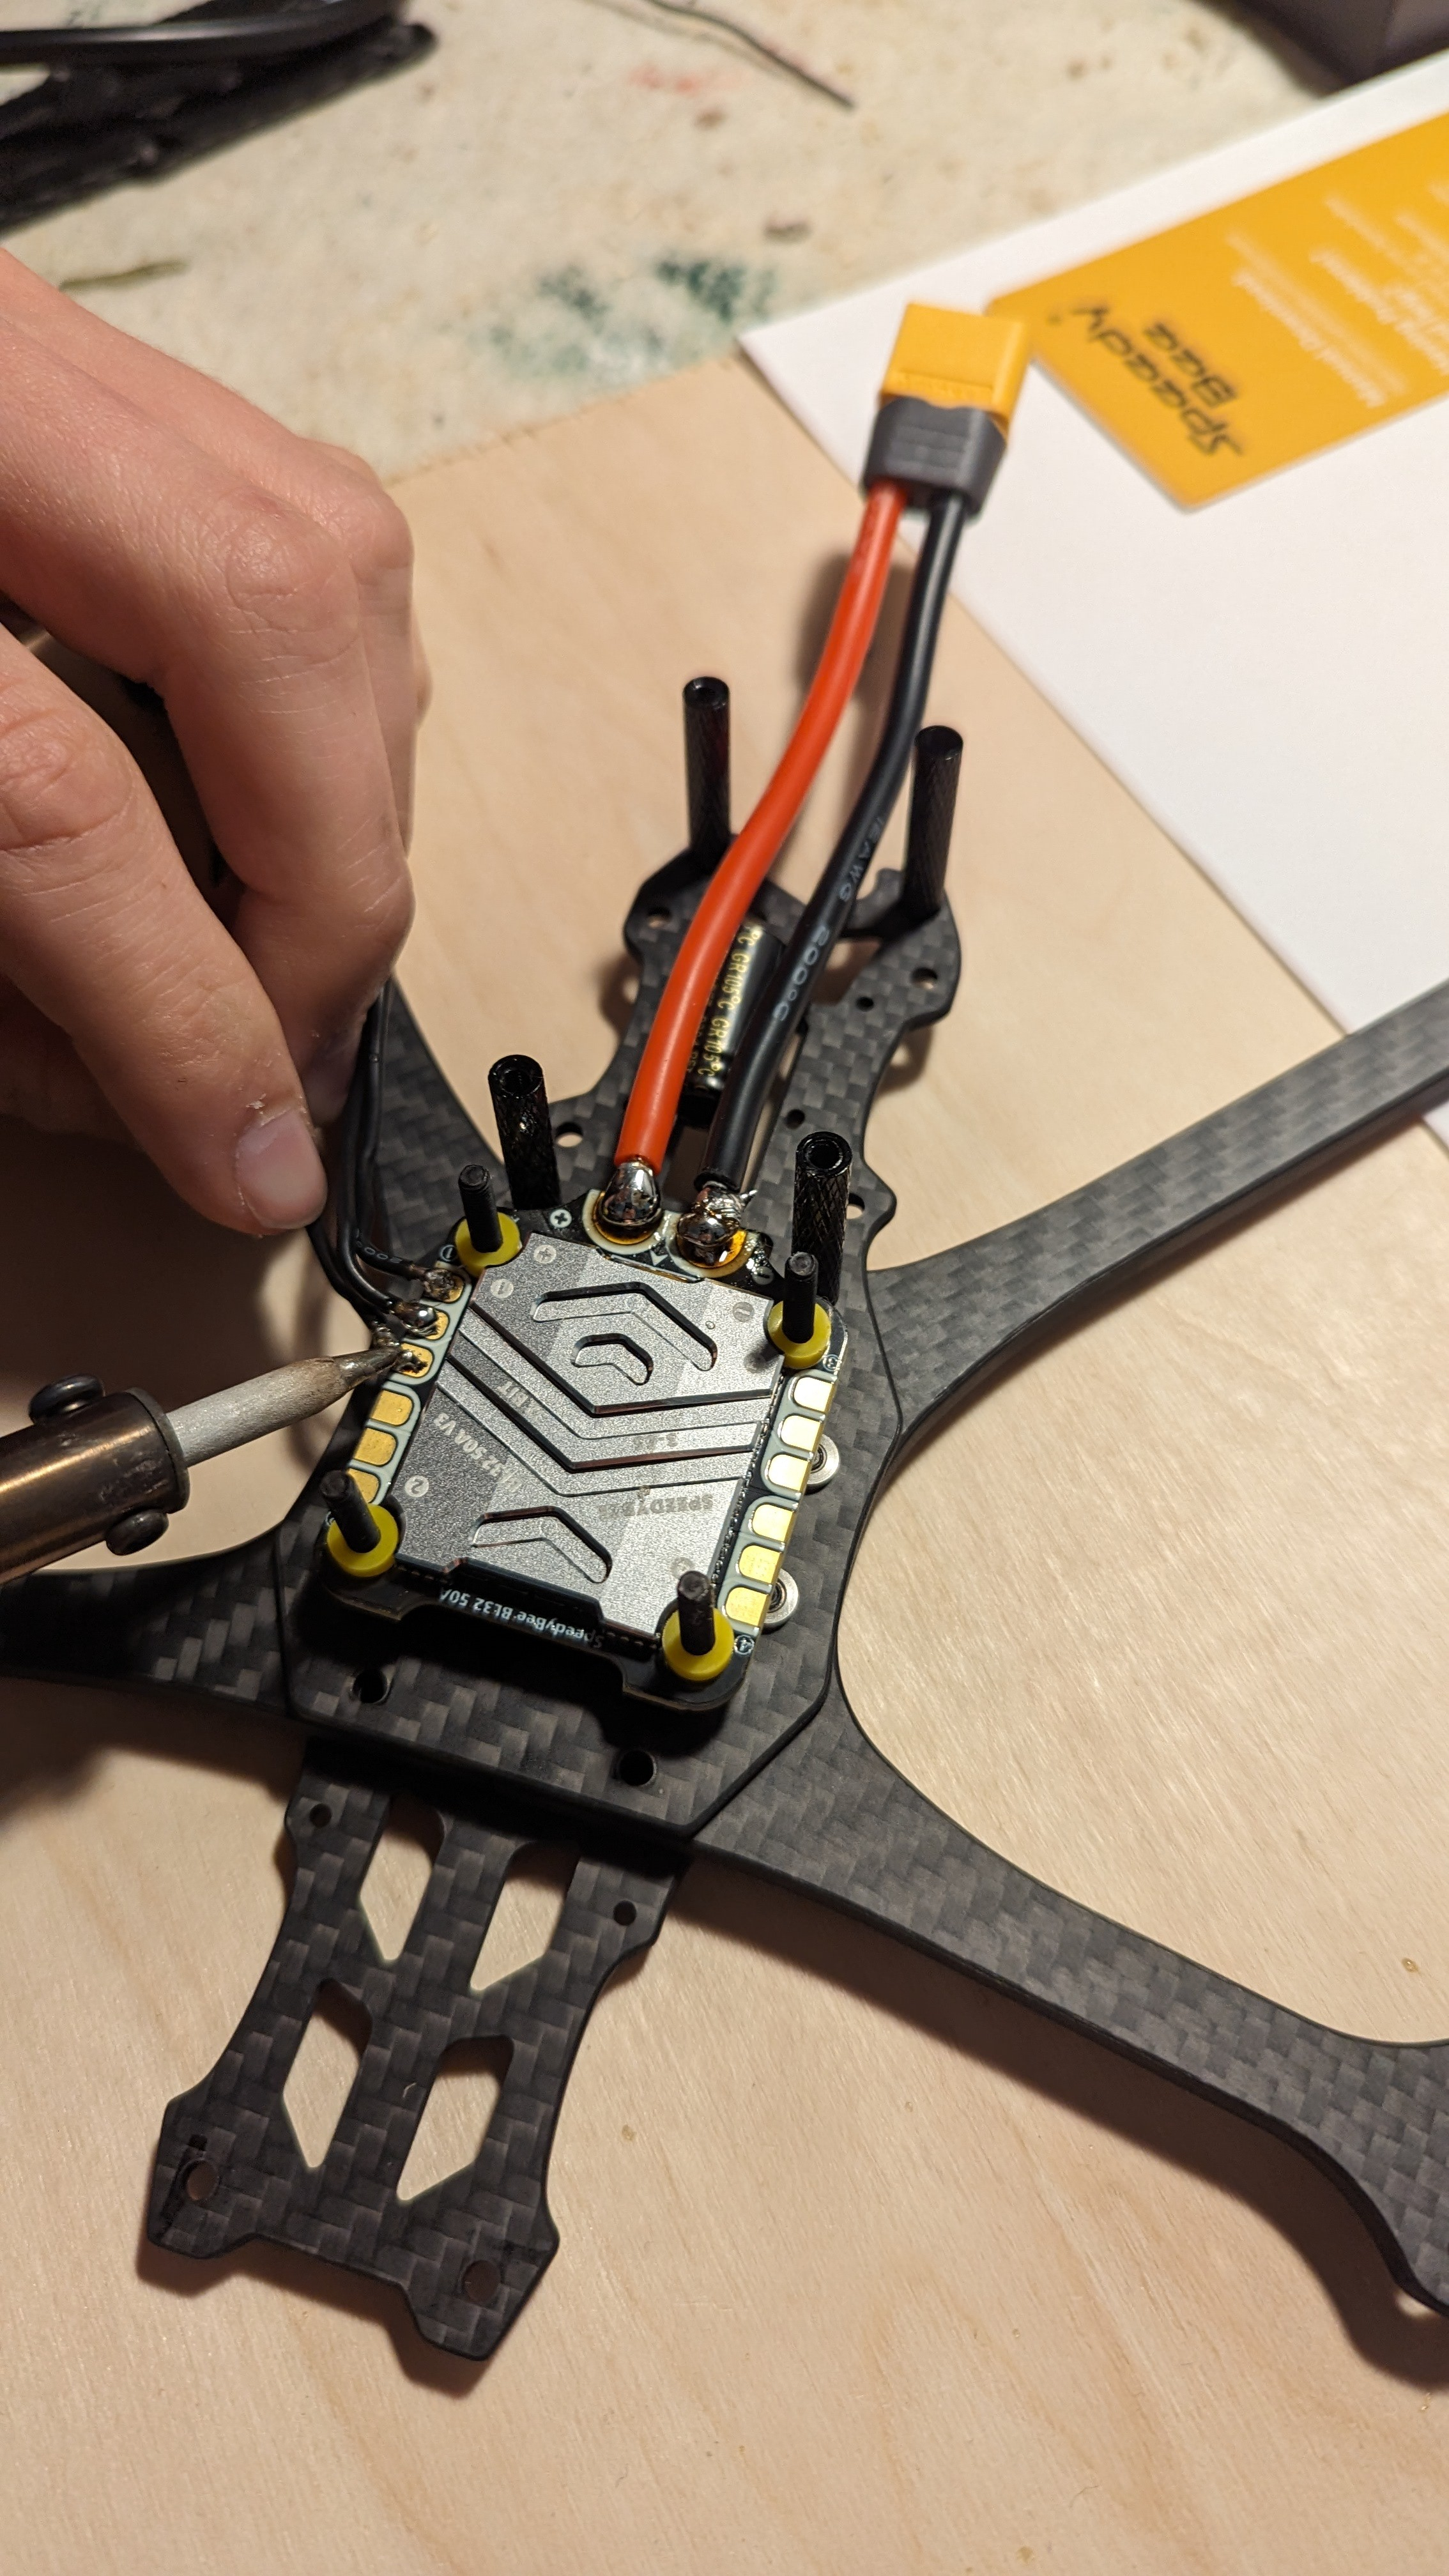
\includegraphics[width=\textwidth]{aufbaubilder/pro-uljbdmei.jpeg}
		\caption{Lötvorgang des ersten Motors.}
		\label{fig:aufbau10}
	\end{minipage}
	
	\vskip 0.5cm % Abstand zwischen den Reihen
\end{figure}
\begin{figure}[htbp]	
	% Vierte Reihe mit drei Bildern
	\begin{minipage}[b]{0.3\textwidth}
		\centering
		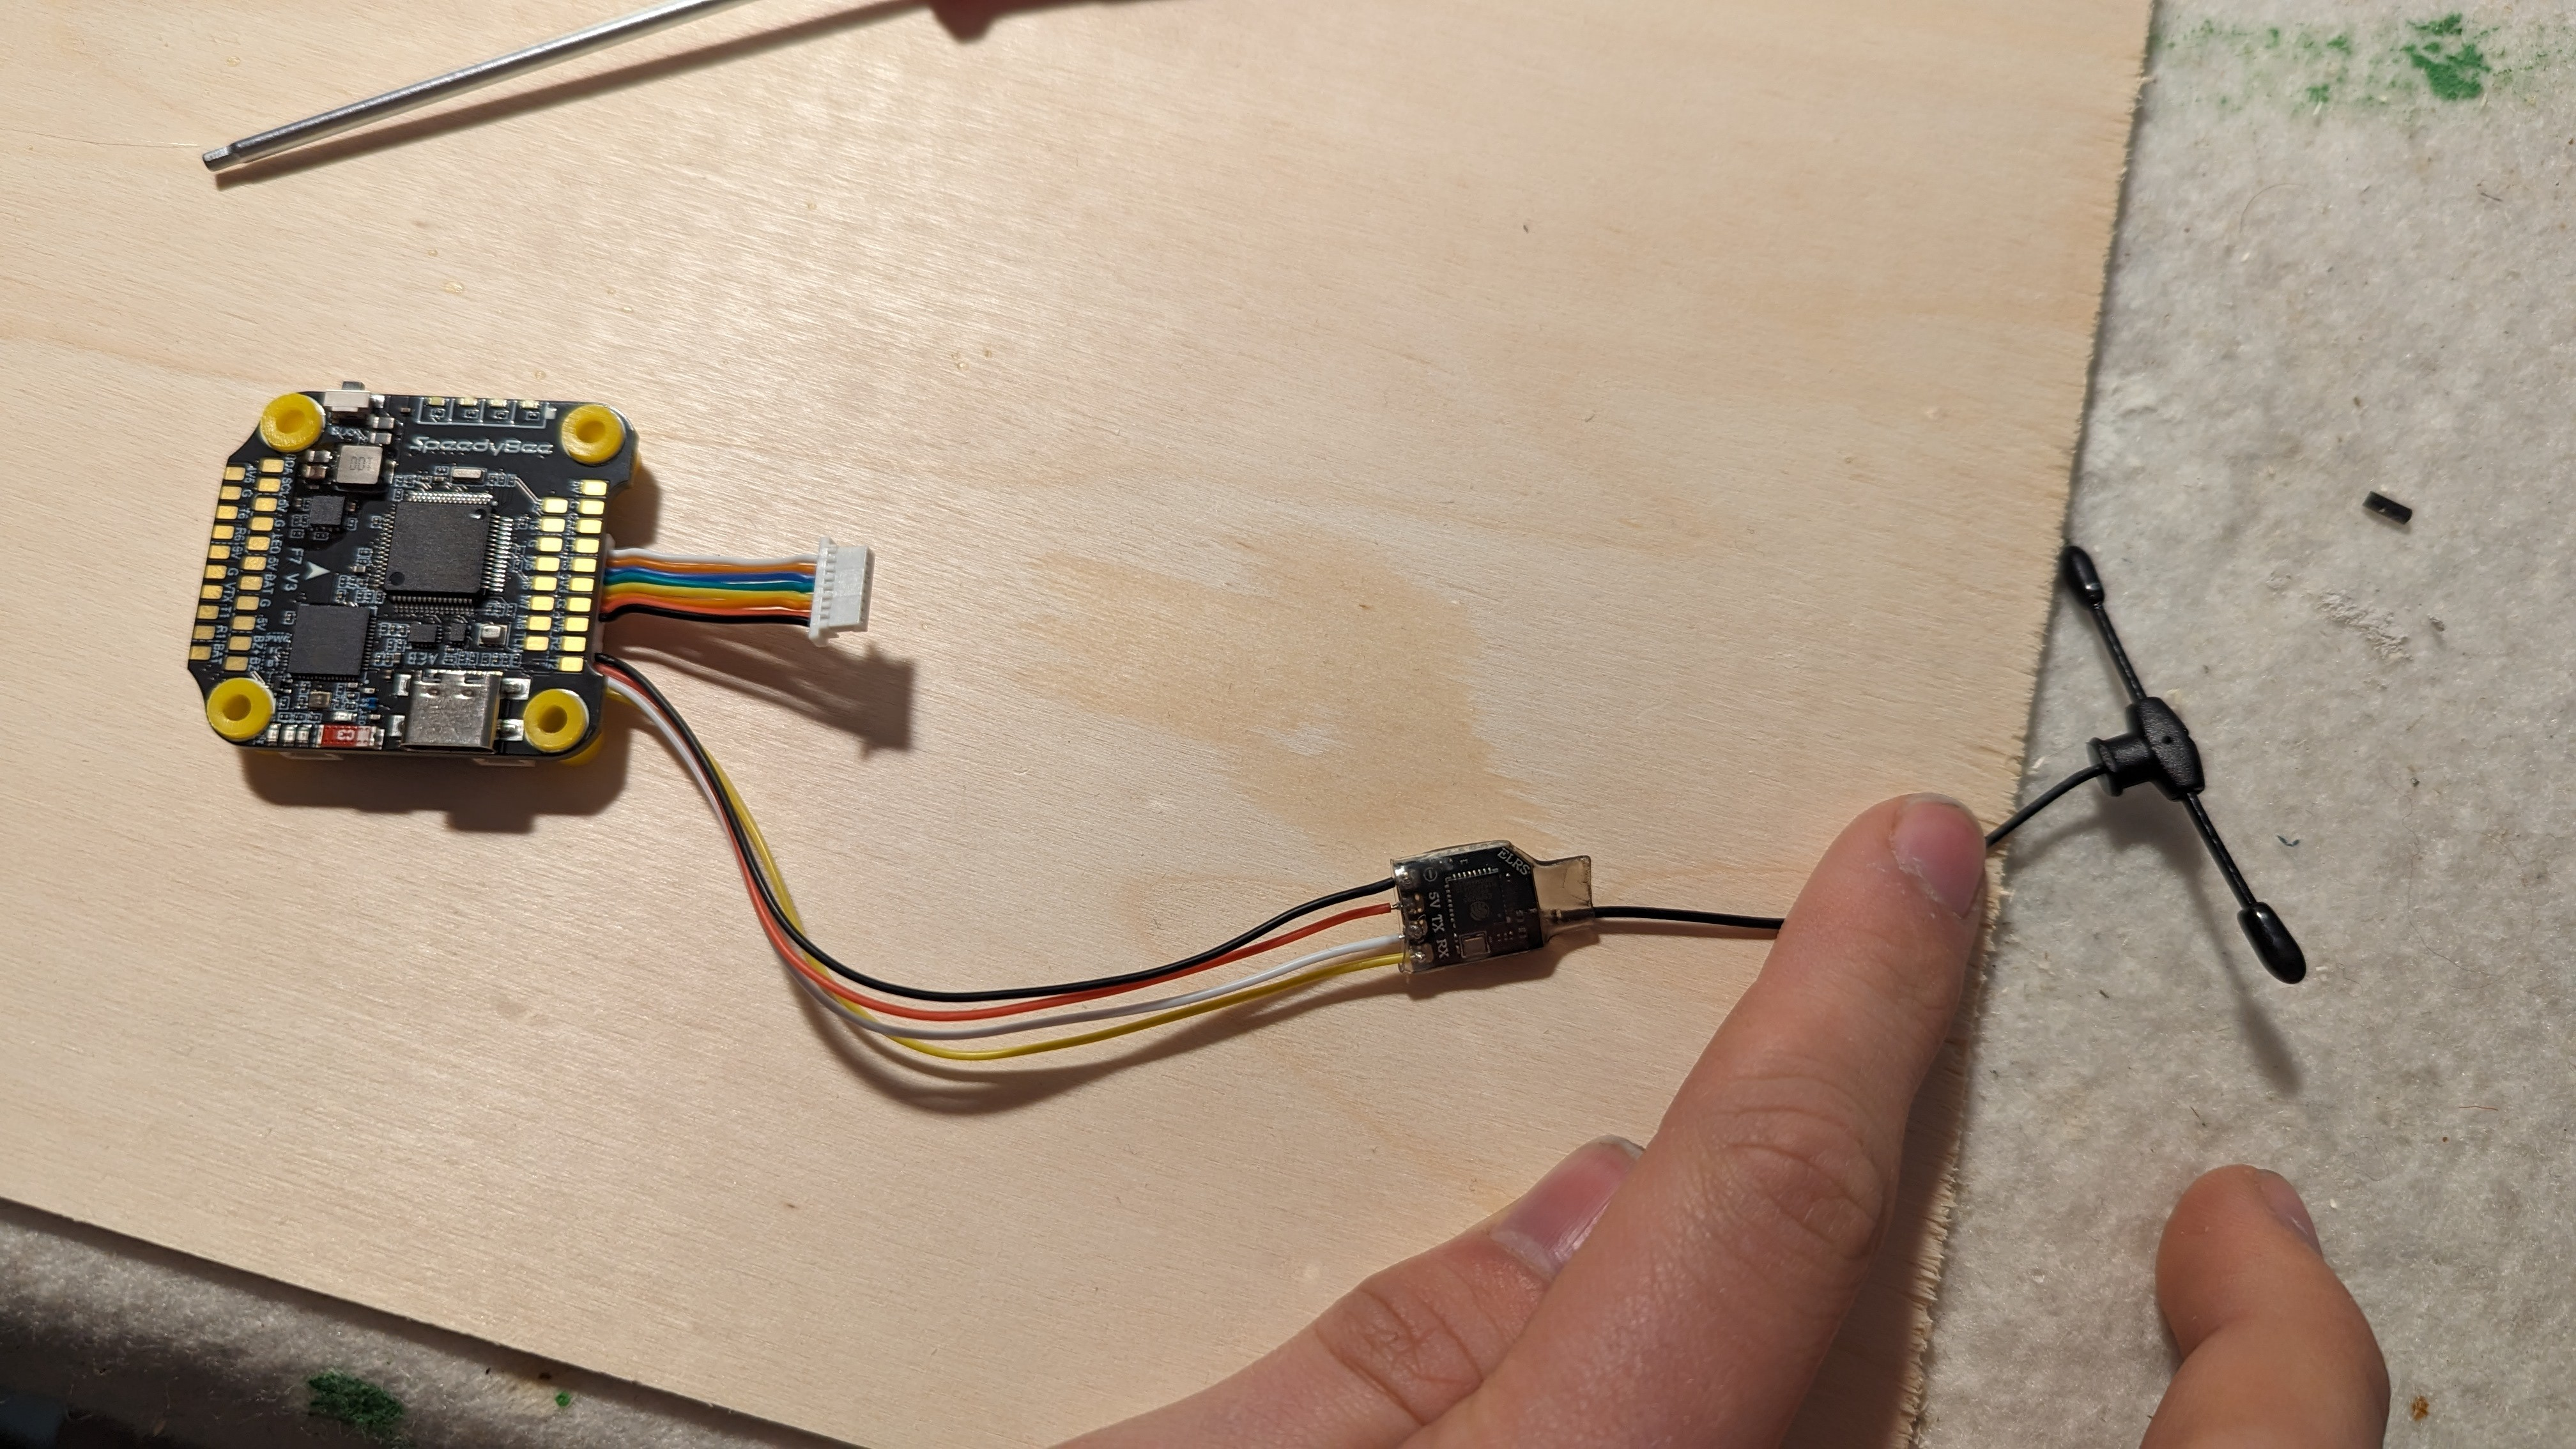
\includegraphics[width=\textwidth]{aufbaubilder/pro-Mrau710H.jpeg}
		\caption{ELRS-Empfänger und Antenne mit dem ESC verbunden.}
		\label{fig:aufbau11}
	\end{minipage}%
	\hfill
	\begin{minipage}[b]{0.3\textwidth}
		\centering
		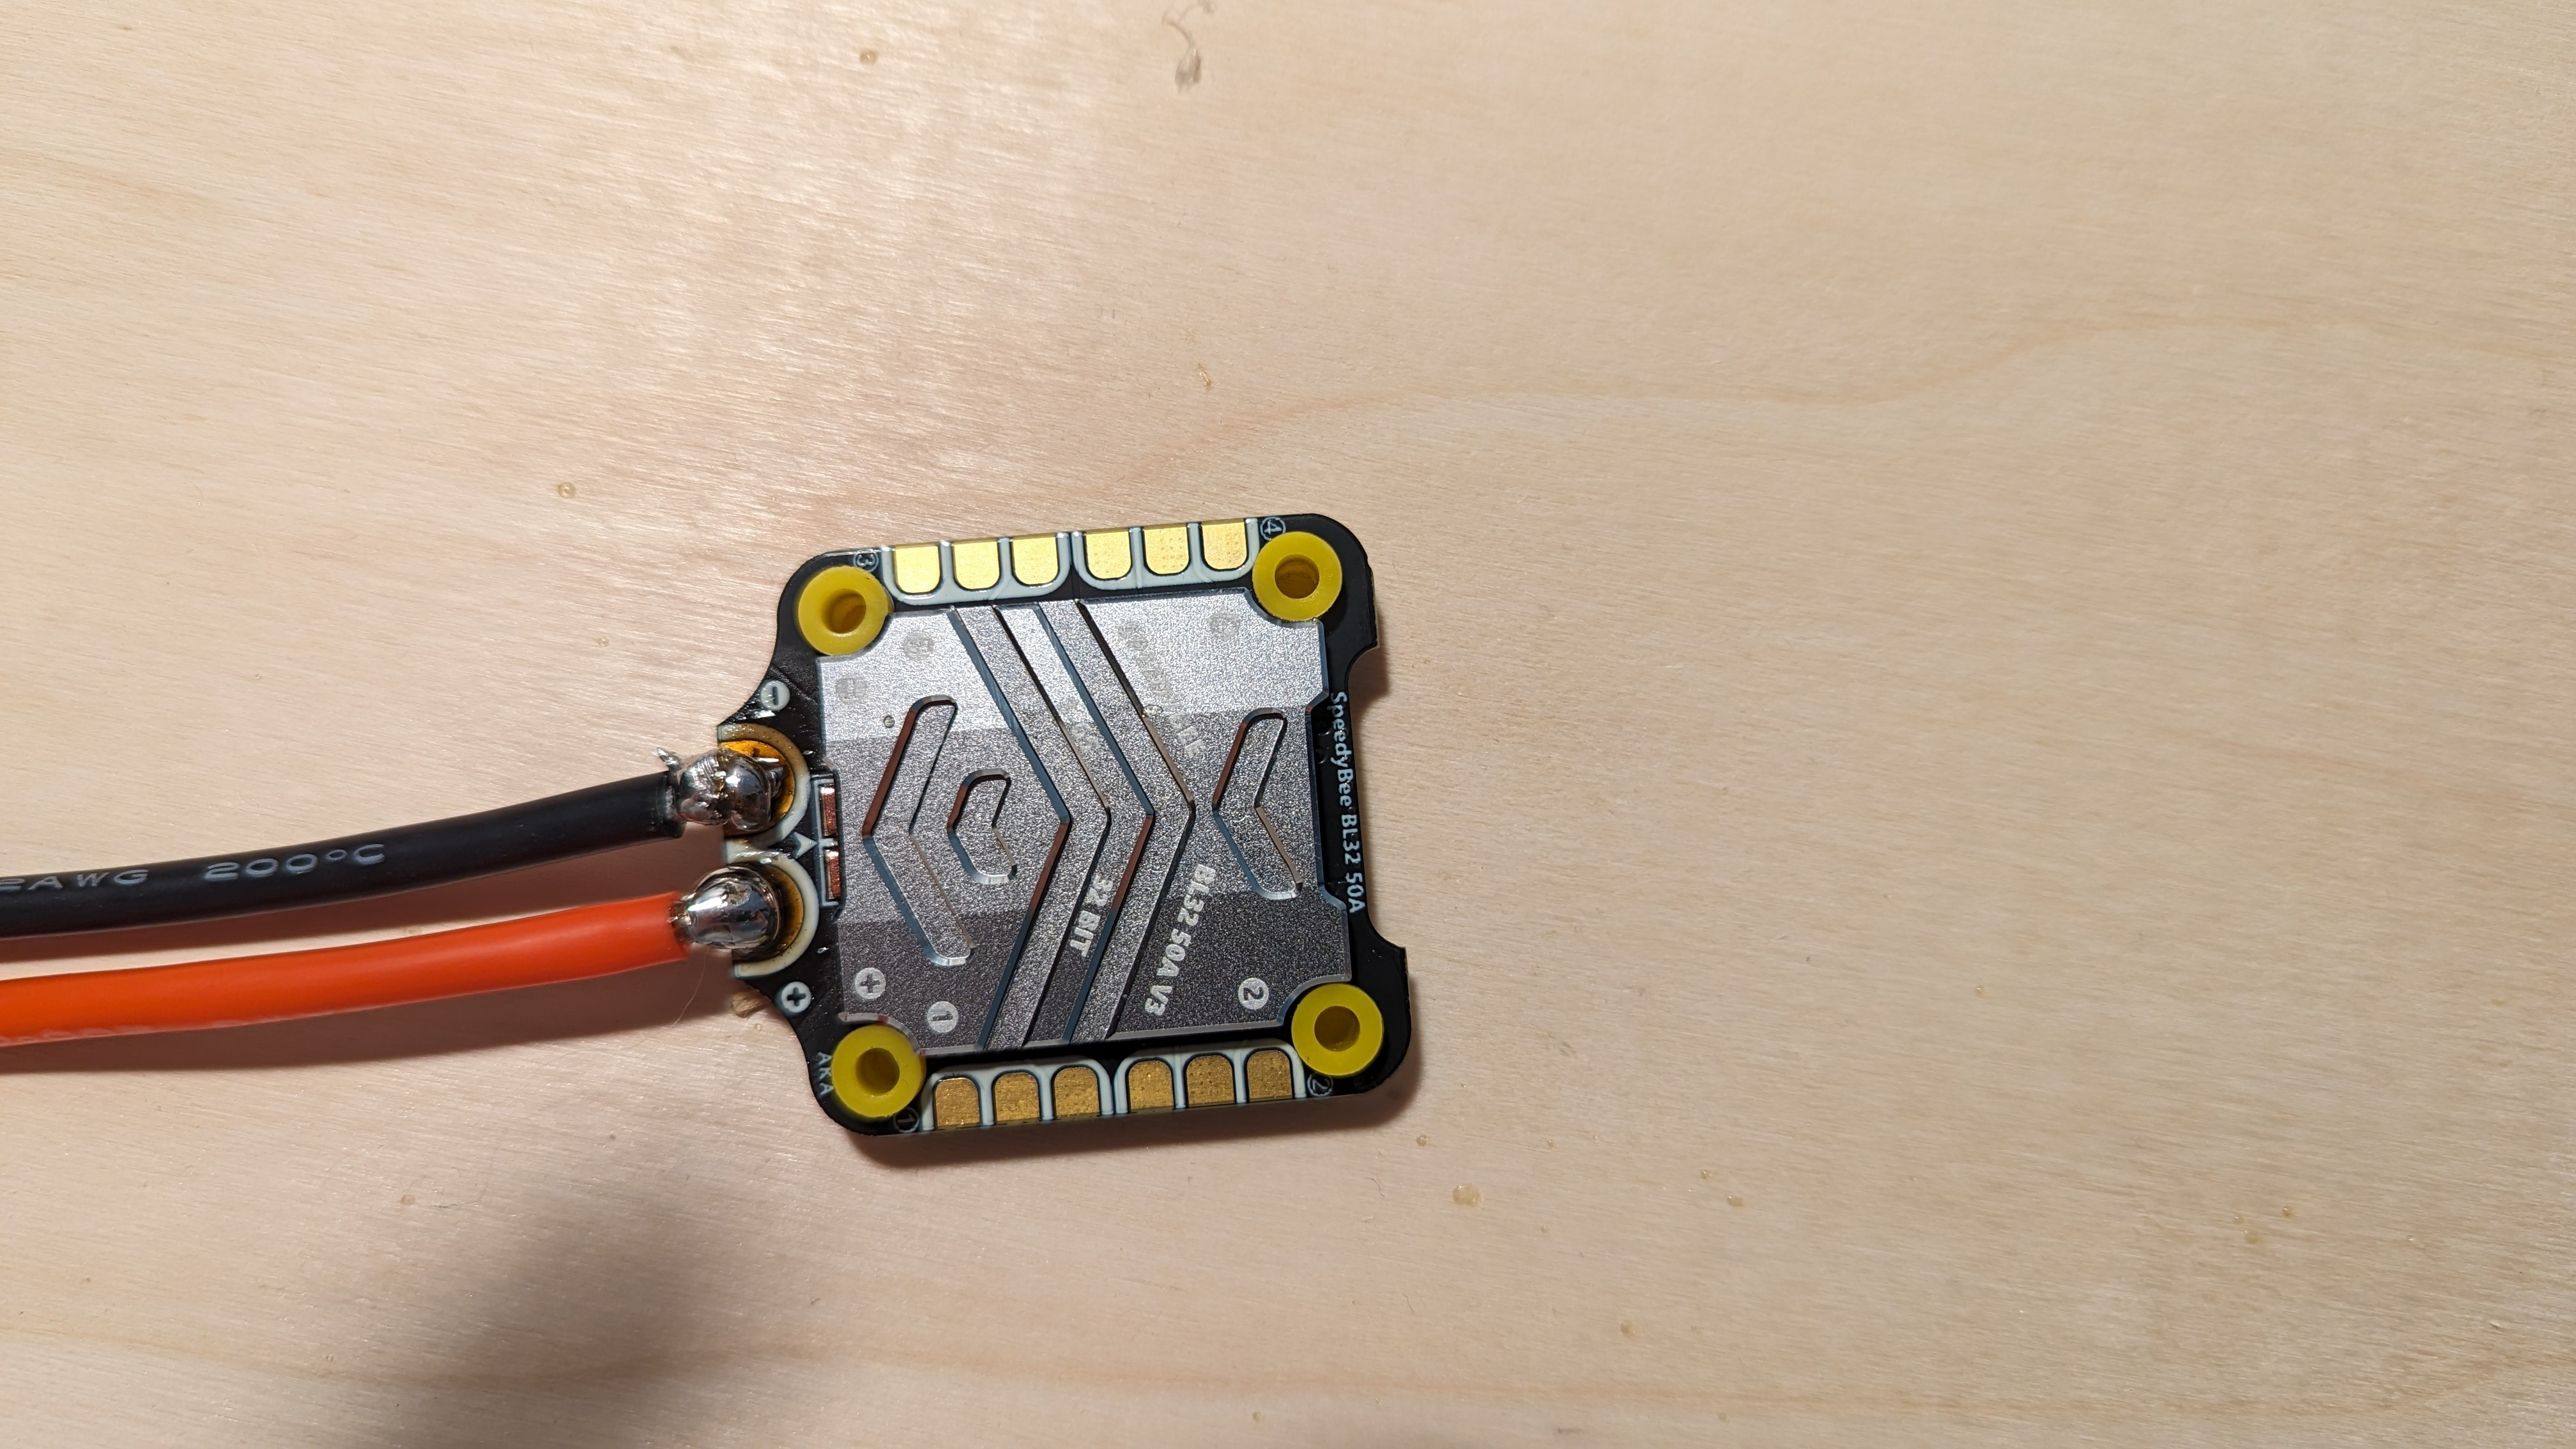
\includegraphics[width=\textwidth]{aufbaubilder/pro-O0D6aZJg.jpeg}
		\caption{Hauptstromversorgung (noch nicht auf der Drohne).}
		\label{fig:aufbau12}
	\end{minipage}%
	\hfill
	\begin{minipage}[b]{0.3\textwidth}
		\centering
		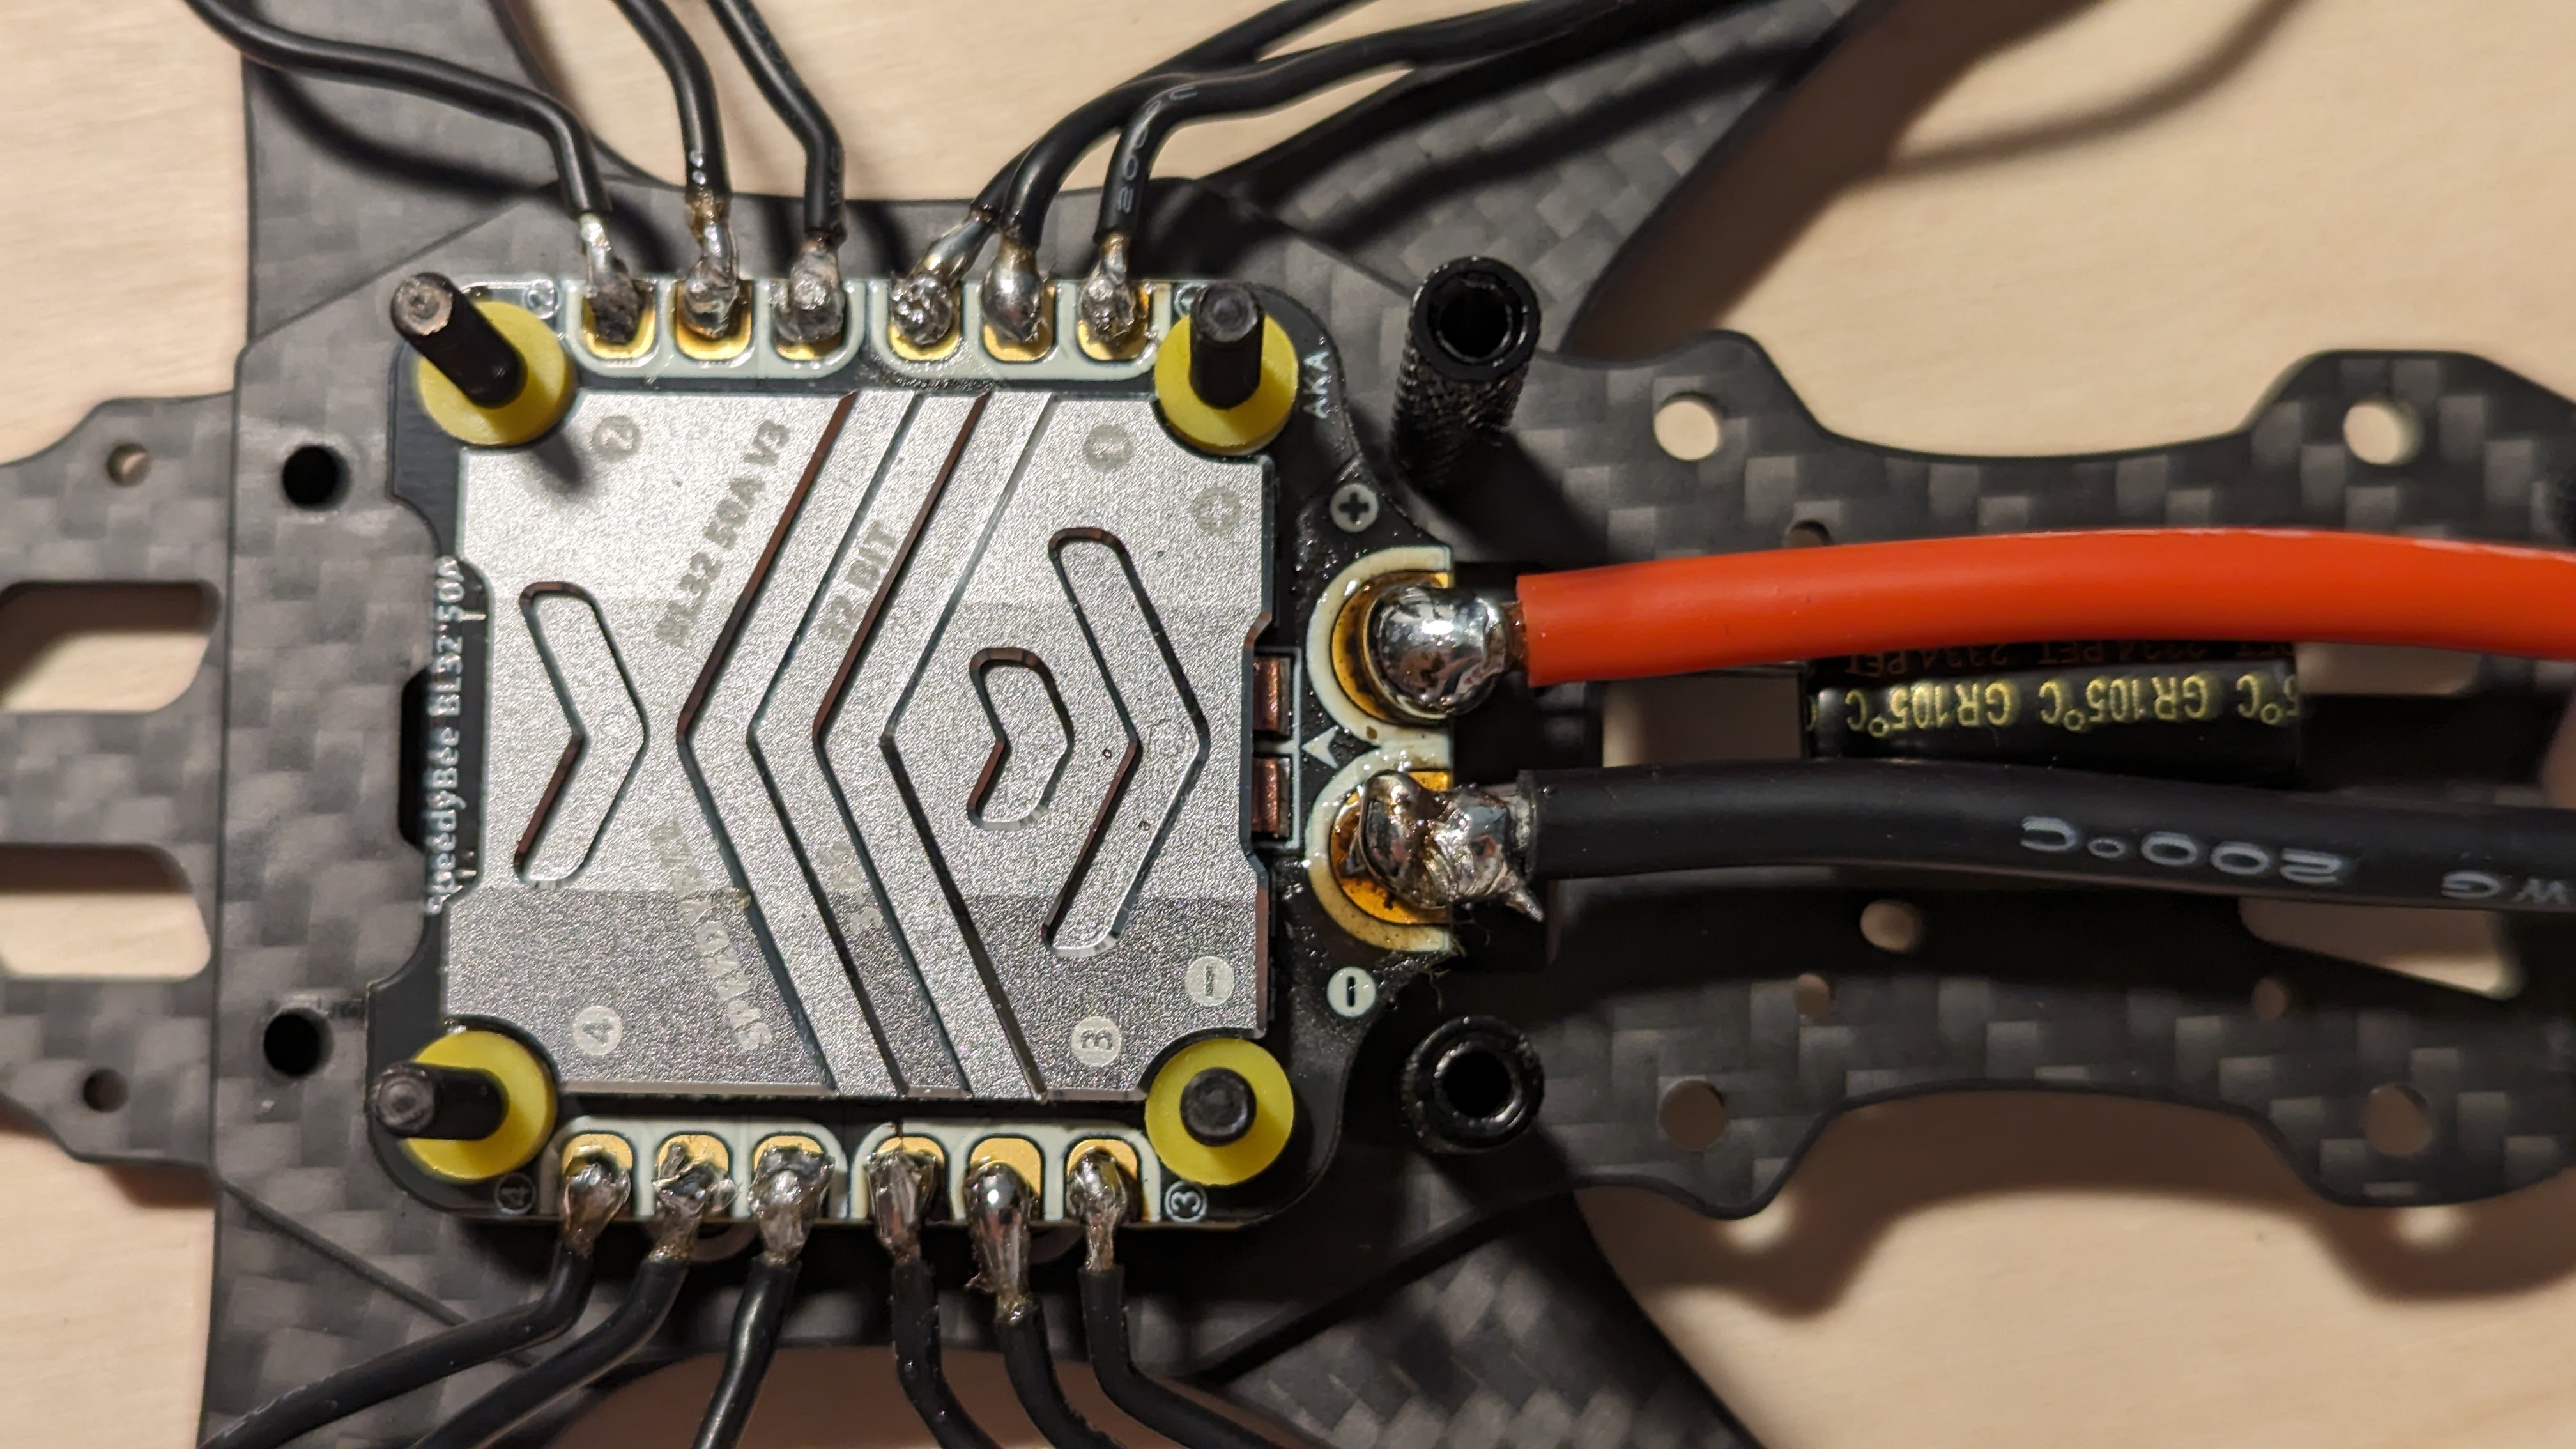
\includegraphics[width=\textwidth]{aufbaubilder/pro-EuLqbThP.jpeg}
		\caption{Draufsicht auf ESC mit allen angelöteten Motoranschlüssen.}
		\label{fig:aufbau13}
	\end{minipage}
\end{figure}

\begin{figure}[htbp]	
	% Vierte Reihe mit drei Bildern
	\begin{minipage}[b]{0.3\textwidth}
		\centering
		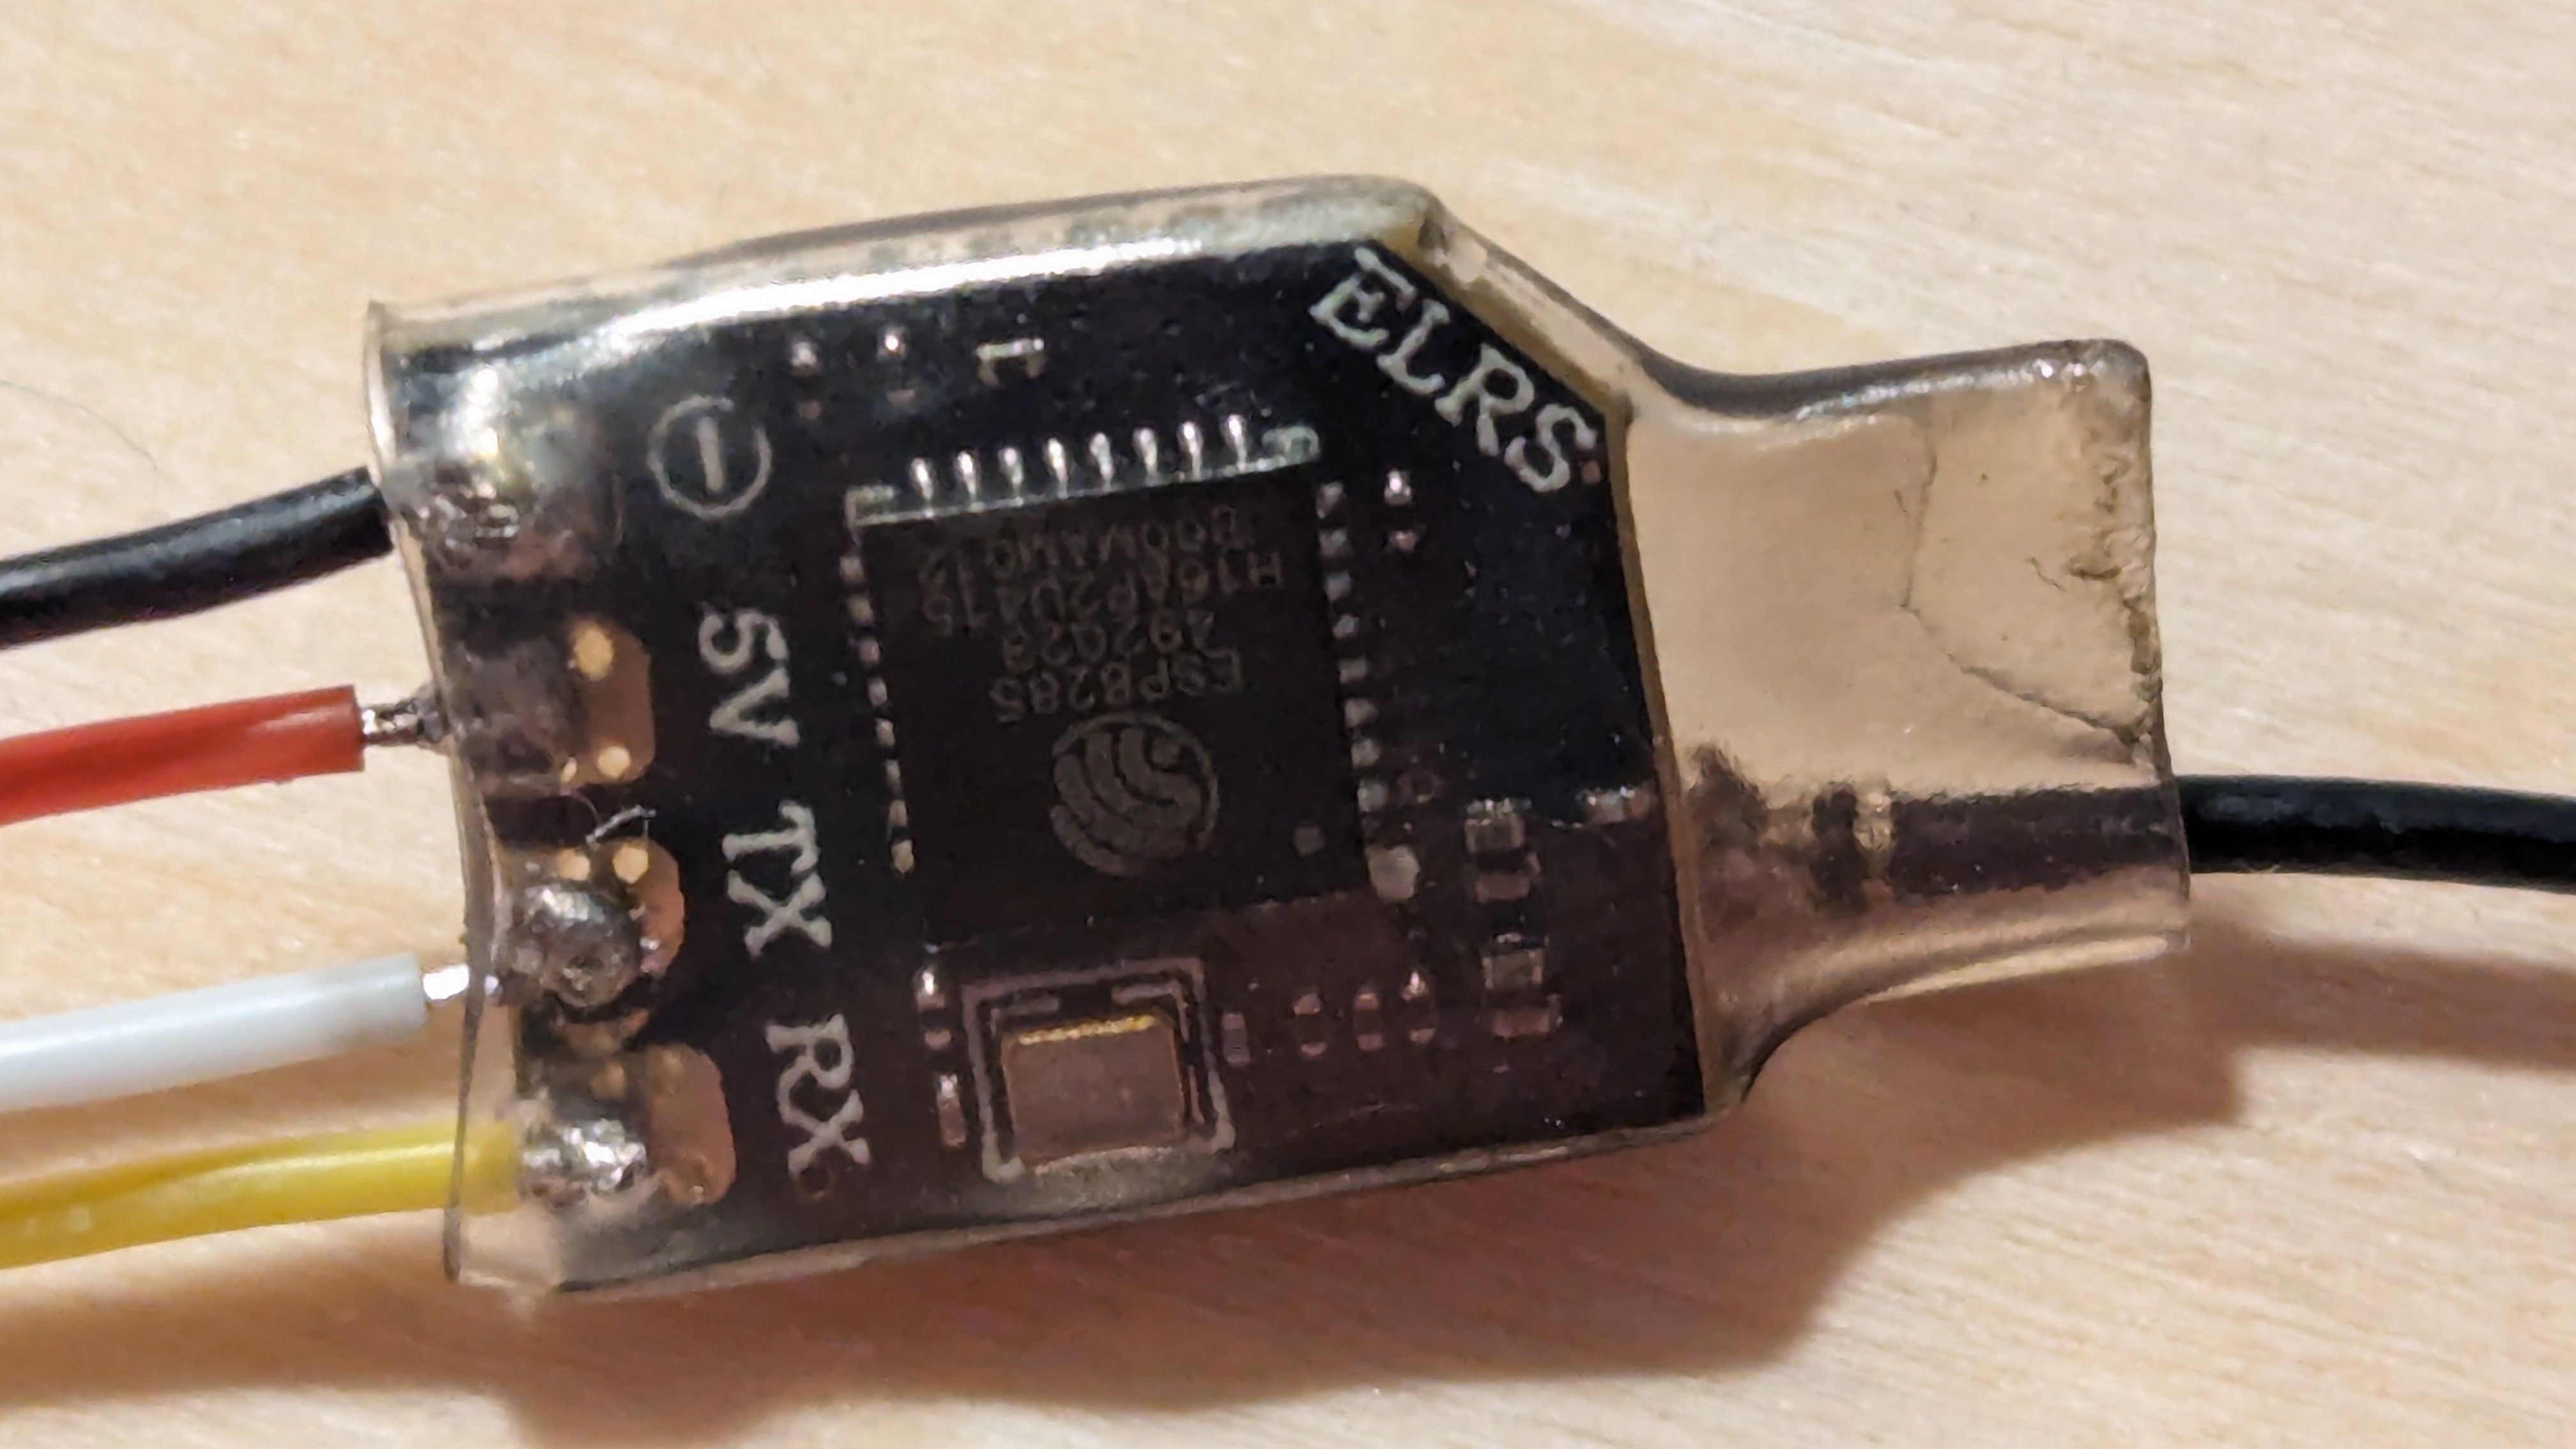
\includegraphics[width=\textwidth]{aufbaubilder/pro-2Vs9jnhc.jpeg}
		\caption{Nahaufnahme des ELRS-Empfängers mit Schrumpfschlauch.}
		\label{fig:aufbau14}
	\end{minipage}%
	\hfill
	\begin{minipage}[b]{0.3\textwidth}
		\centering
		\includegraphics[width=\textwidth]{aufbaubilder/lötstation.jpg}
		\caption{Lötstation.}
		\label{fig:aufbau15}
	\end{minipage}%
	\hfill
	\begin{minipage}[b]{0.3\textwidth}
		\centering
		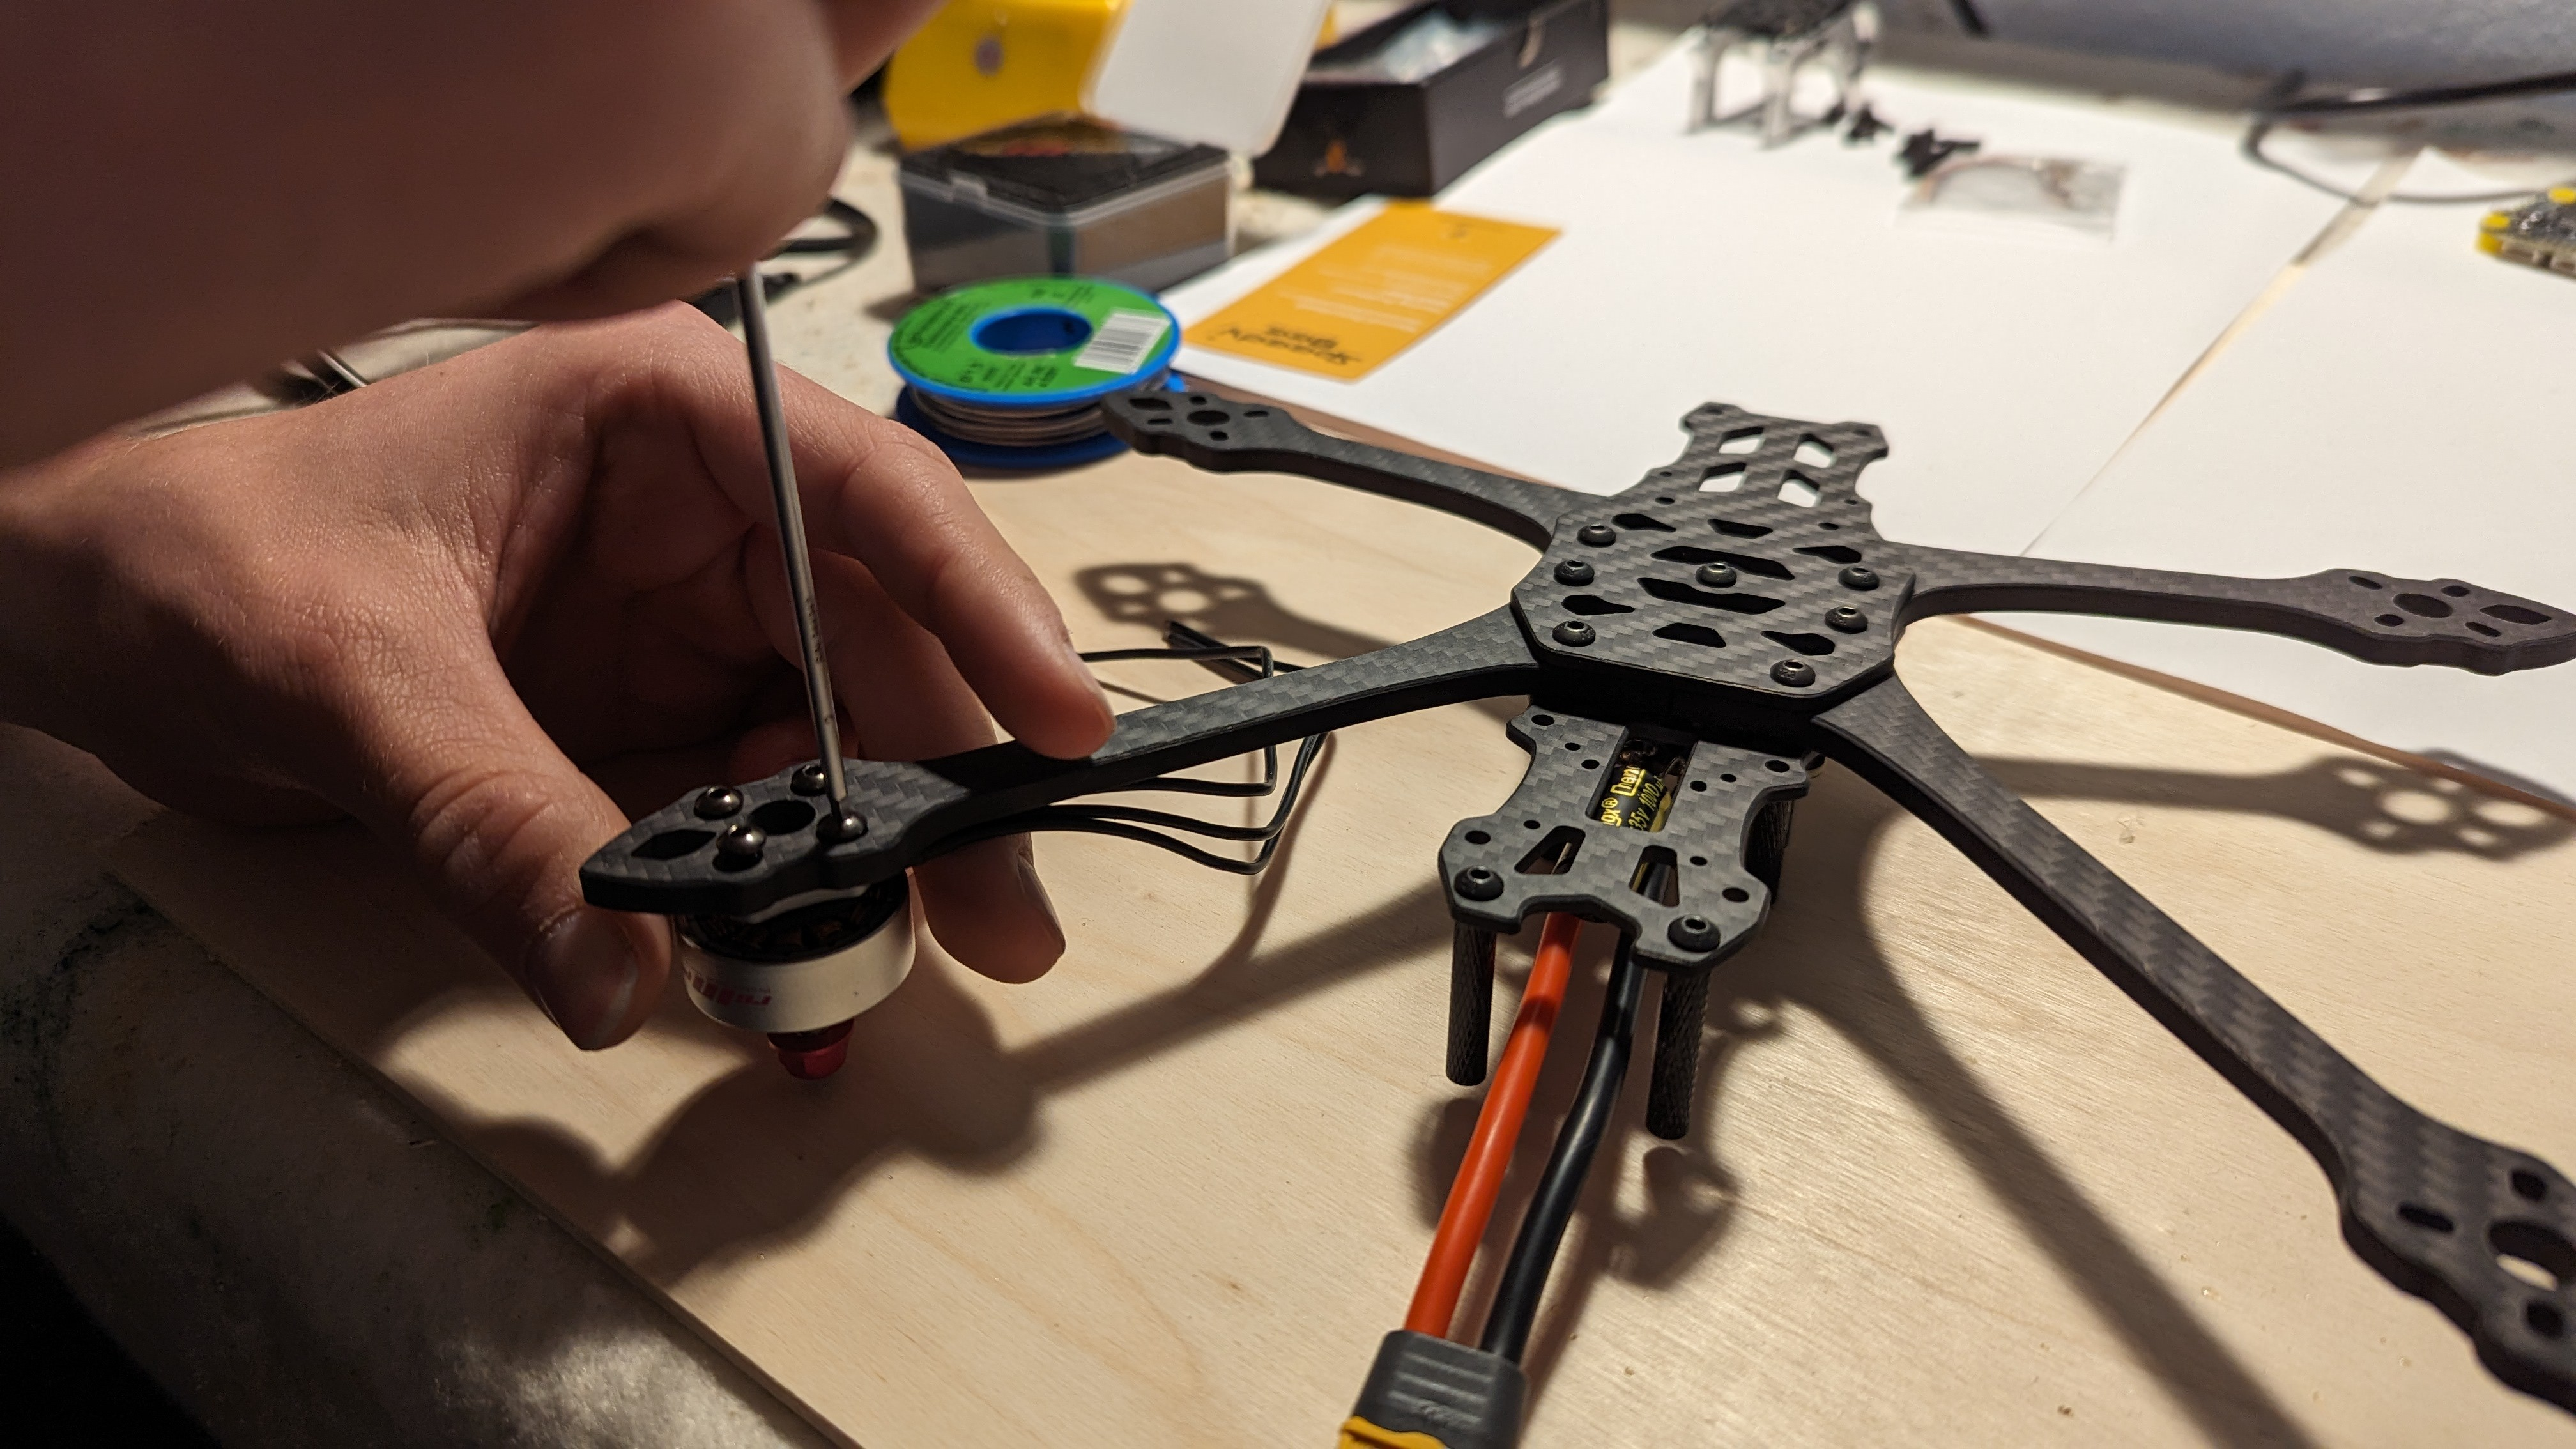
\includegraphics[width=\textwidth]{aufbaubilder/pro-meIUnESh.jpeg}
		\caption{Anschraubprozess des ersten Motors.}
		\label{fig:aufbau16}
	\end{minipage}
\end{figure}











% =========== ENDE VON ANHÄNGE ============



% =============================================================
\end{document} % ENDE VOM DOKUMENT ============================
% =============================================================
